\documentclass{tudelft-report}

%% Set up the bibliography
\usepackage[style=authoryear]{biblatex}
\addbibresource{report.bib}

%% Additional packages and commands
\usepackage{parskip}
\setlist{itemsep=-2pt} % Reducing white space in lists slightly
\renewcommand{\deg}{\si{\degree}\xspace} % Use \deg easily, everywhere

% \usepackage{ctex}
\usepackage[figuresright]{rotating}
%% ----------------------------------------------------------------------
%%    Begin of document + Frontmatter (Roman page numbering)
%% ----------------------------------------------------------------------

\begin{document}

\frontmatter

%% Define the main parameters
\title{Replication Report}
\subtitle{Sovereign Debt Relief and Its Aftermath }
\author{Carmen M. Reinhart \\
Christoph Trebesch}

% \footnotetext[1]{Harvard University, Kennedy School}
% \footnotetext[2]{University of Munich}

% \subject{AB1234: Optional Course Name} % Cover only
% \affiliation{Delft University of Technology} % Cover only
% % \coverimage{figures/cover.jpg} % Aspect ratio of 2:3 (portrait) recommended
% \definecolor{title}{HTML}{4884d6} % Color for cover title

% \makecover

\begin{titlepage}

\begin{center}

%% Print the title
{\makeatletter
\largetitlestyle\fontsize{45}{45}\selectfont\@title
\makeatother}

%% Print the subtitle
{\makeatletter
\ifdefvoid{\@subtitle}{}{\bigskip\titlestyle\fontsize{20}{20}\selectfont\@subtitle}
\makeatother}

\bigskip
\bigskip

by

\bigskip
\bigskip

%% Print the name of the author
{\makeatletter
\largetitlestyle\fontsize{25}{25}\selectfont\@author
\makeatother}

\bigskip
\bigskip

%% Print table with names; easily add columns if necessary or remove the table completely
\setlength\extrarowheight{2pt}
\begin{tabular}{l}
    Fu Jingle \\
    Zhang Yingjie \\
\end{tabular}

\vfill

%% Print some more information at the bottom
\begin{tabular}{ll}
    Instructor: & Michele Pellizzari \\
    Teaching Assistant: & Houssein Tohidimehr \\
    % Project Duration: & Month, Year - Month, Year \\
    % Faculty: & Faculty of Aerospace Engineering, Delft
\end{tabular}

\bigskip
\bigskip

%% Add a source and description for the cover and optional attribution for the template
% \begin{tabular}{p{15mm}p{10cm}}
%     Cover: & Canadarm 2 Robotic Arm Grapples SpaceX Dragon by NASA under CC BY-NC 2.0 (Modified) \\
%     % Feel free to remove the following attribution, it is not required - still appreciated :-)
%     Style: & TU Delft Report Style, with modifications by Daan Zwaneveld
% \end{tabular}

\end{center}

%% Insert the TU Delft logo at the bottom of the page
% \begin{tikzpicture}[remember picture, overlay]
%     \node[above=10mm] at (current page.south) {%
%         \includegraphics{figures/logo-black}
%     };
% \end{tikzpicture}

\end{titlepage}

% \begin{myminipage} 
     This is the lecture note taken in the course \textit{\courseloc} taught by \profloc{} at \instituteloc{} as part of the \classloc{} program (\sessionloc).
     The content is partly based on the course notes provided by the professor and supplemented by many other references I read myself. The main reason is that the original notes are found a bit ambiguous
     and I want to further clarify.

     Currently, these are just drafts of the lecture notes. There can be typos and mistakes anywhere. So, if you find anything that needs to be corrected or improved, please inform at \myemailloc. \bigskip

     % I am deeply grateful to my late friend, Gilles Castel, who introduced me to \LaTeX{} for the first time.
\end{myminipage}

% \chapter*{Summary}
\addcontentsline{toc}{chapter}{Summary}

本报告旨在复现Reinhart和Trebesch (2016)关于主权债务减免及其经济后果的核心研究思路、模型选择逻辑和关键数学推导。
论文通过对两次截然不同的历史时期(1920-1939年发达经济体的官方债务违约和1978-2010年新兴市场的私人外部债权人债务危机)进行量化分析,揭示了债务减免的规模和影响。
核心发现是,只有涉及债务注销(debt write-offs)的债务减免操作才能显著改善债务国的经济状况,而诸如期限延长和利率削减等较温和的债务减免形式通常不会带来经济增长的显著提高或信用评级的改善。

本报告还将探讨在原文经典双重差分(DiD)方法基础上,应用交错双重差分(Staggered DiD)方法进行分析的潜力及其数学框架。

\tableofcontents
%\listoffigures
%\listoftables

% \chapter*{Nomenclature}
\addcontentsline{toc}{chapter}{Nomenclature}

\emph{If a nomenclature is required, a simple template can be found below for convenience. Feel free to use, adapt or completely remove.}

\section*{Abbreviations}

\begin{longtable}{p{2.5cm}p{8cm}}
    \toprule
    Abbreviation & Definition \\
    \midrule\endhead % Add abbreviations alphabetically here:
    ISA & International Standard Atmosphere \\
    ... \\
    \bottomrule
\end{longtable}

\section*{Symbols}

\begin{longtable}{p{2.5cm}p{8cm}p{2.5cm}}
    \toprule
    Symbol & Definition & Unit \\
    \midrule\endhead % Add Latin symbols alphabetically here:
    $V$ & Velocity & [m/s] \\
    ... \\
    \midrule % Add Greek symbols alphabetically here:
    $\rho$ & Density & [kg/m$^3$] \\
    ... \\
    \bottomrule
\end{longtable}


%% ----------------------------------------------------------------------
%%    Mainmatter (Arabic page numbering)
%% ----------------------------------------------------------------------

\mainmatter

\chapter{Introduction}
\label{chapter:introduction}

\section{Key question}

Should countries with a heavy debt burden and little prospect of repayment receive debt forgiveness?

The literature has mostly focused on the occurrence of debt crises, but not on their resolution.

\underline{\textbf{Contribution of this paper:}}
filling this gap by studying two 20th century instances of debt relief
that encompassed a substantial number of countries.

\begin{enumerate}
    \item Quantifying the scale of debt relief: Sovereign debt relief was quantified for two important historical periods:
        \begin{itemize}
            \item The default on official debts by advanced economies after World War I (1920-1939).
            \item The debt crises faced by emerging markets in recent decades with private external creditors (1978-2010).
        \end{itemize}
        % 一个是第一次世界大战后发达经济体对官方债务的违约(1920-1939)
        % 另一个是近几十年来新兴市场对私人外部债权人的债务危机(1978-2010)
    \item Document the process and magnitude of debt relief achieved through default and restructuring of external sovereign debt in 48 crisis spells.
        During World War I, it was dominated by official external sovereign debt (i.e., debts owed to government creditors). \\
        \emph{Reminds the situation in periphery Europe today, where much of the debts are now also in the hands of official creditors. 
        Moreover, it is notable that the episode ended with a full cancellation of the war debt.}
    \item Analyzing the economic consequences of debt relief: Special attention is paid to the impact of debt relief operations (especially debt write-offs)
    on a country's macroeconomic performance (GDP per capita growth, sovereign credit ratings, debt servicing costs, debt levels).
    % 分析债务减免的经济后果: 特别关注债务减免操作(尤其是债务注销)对国家宏观经济表现
    % (人均GDP增长、主权信用评级、偿债成本、债务水平)的影响。
    % \item 方法论: 采用双重差分(DiD)方法,利用历史上几次同步的、由外部力量(如美国政府)协调的债务减免事件作为自然实验,
    % 以减轻内生性问题。
\end{enumerate}

\section{Key Challenges}

\begin{enumerate}
    \item Timing of debt relief may be endogenous.
        \emph{Solution:} focus on episodes of debt reduction that were synchronously applied across debtor countries,
        regardless of individual economic circumstances
        \begin{itemize}
            \item 1931 Hoover Moratorium: cash flow relief (debt service moratorium).
            \item 1934 General Default on War Debts: debt stock relief (debt write-off).
            \item 1986 Baker Plan: reducing interest rates and lengthening maturities.
            \item 1990 Brady Initiative: face value debt reduction.
        \end{itemize}
    \item Omitted variables and other factors.
        \emph{Solution:} Add time and country fixed effects.
        And use robustness checks: adding controls for inflation, banking crises, currency crises, wars and conflicts, and major political shocks
\end{enumerate}

% \section{作者研究思路、逻辑、模型选择与意图分析}

\begin{itemize}
    \item \textbf{Logic and Motivation}:  
    First, the authors must demonstrate that the debt-relief episodes under study were historically \emph{important} and \emph{large enough} to warrant close scrutiny.  
    They do so by conducting an extensive survey of the historical literature and by building a new two-period database on debt relief.

    \item \textbf{1920-1939: Official Debt of Advanced Economies}%
        \begin{itemize}
            \item \textbf{Data collection}: 18 advanced debtor countries vis-à-vis the two main creditor nations after World War~I—the United States and the United Kingdom\footnote{For details on official lending and debt-relief events in the dense network of war-related loans, see the online appendix.}.
            % Data sources: U.S.\ Treasury Annual Reports, Moody’s Foreign Government Bond Manuals, various League of Nations publications, etc.
            \item \textbf{Quantifying relief}: Focus on the widespread default and cancellation of war debts owed to the U.S.\ and the U.K.\ in 1934.
                \begin{itemize}
                    \item \emph{Preferred measure}: face value of outstanding war debts as a share of GDP, because these debts were eventually written off in full.
                    \item \emph{Alternative measure}: present-value relief calculated under the 1920s restructuring terms, using the 5\% discount-rate approach of Moulton and Pasvolsky (1932), which delivers a conservative lower bound.
                \end{itemize}
            \item \textbf{Model-selection rationale}: When a debt is completely cancelled, face value equals the amount relieved. Present-value calculations facilitate comparison with the ``haircut'' concept in emerging markets and show that the magnitude remains large even under cautious assumptions.
        \end{itemize}

    \item \textbf{1978-2010: Private Creditors—Foreign Banks and Bondholders (Emerging-Market Debt)}%
        \begin{itemize}
            \item \textbf{Data collection}: relies on earlier estimates of haircuts in middle-income emerging markets between 1978 and 2010.\footnote{The pioneering study computes several measures of debt relief for a representative set of crises and countries, and documents the crisis-resolution process in detail.}
            \item \textbf{Data source}: the Cruces and Trebesch (2013) database, which builds on the haircut methodology of Sturzenegger and Zettelmeyer (2006, 2007, 2008).
            \item \textbf{Quantifying relief}: cumulative \emph{effective haircut} over the entire default spell, taking account of multiple sequential restructurings.
                \begin{itemize}
                    \item \emph{Model-selection rationale}: Emerging-market restructurings typically exchange old bonds for new ones and combine nominal write-downs, maturity extensions, or coupon reductions.  The haircut provides a standardised metric of investor losses; its cumulative version captures the \emph{total} debt relief achieved during crisis resolution.
                \end{itemize}
            \item \textbf{Debt relief-to-GDP ratio}: multiply the cumulative haircut by the face value of affected debt, then divide by nominal GDP.
        \end{itemize}
\end{itemize}


% \subsection{阶段一:历史背景与债务减免的量化 (Historical Context and Quantification of Debt Relief)}
% \begin{itemize}
%     \item 逻辑与意图: 首先,作者需要证明所研究的债务减免事件在历史上是重要的,
%     并且其规模是可观的,值得深入研究。他们通过详细的历史文献回顾和数据收集,构建了两个时期的债务减免数据库。
%     \item 1920-1939: Official debt of advanced economies %发达经济体官方债务:
%         \begin{itemize}
%             \item Data colloction: 18 advanced debtor countries to the two main creditor countries during World War I and the 1920s: the US and the UK\footnote{details on official lending and debt relief events in a large network of war-related loans}.
%             % \item 数据来源: 美国财政部年度报告、穆迪外国政府证券手册、联合国出版物等。
%             \item 减免量化: 主要关注1934年各国对美国和英国的战争债务的普遍违约和注销。
%                 \begin{itemize}
%                     \item 首选方法: 将未偿战争债务的面值(face value)占GDP的比例作为减免规模的度量,因为这些债务最终被完全注销。
%                     \item 备选方法: 计算这些债务在1920年代重组条款下的现值(present value)减免,使用Moulton and Pasvolsky (1932)的5\%贴现率方法作为下限估计。
%                 \end{itemize}
%             \item 模型选择逻辑: 对于完全注销的债务,面值即为减免额。现值计算是为了与新兴市场的“haircut”概念进行某种程度的对比,并展示即使在保守估计下减免规模依然巨大。
%         \end{itemize}
%     \item 1978-2010: Private creditors, notably foreign banks and bondholders (新兴市场私人债务):
%         \begin{itemize}
%             \item Data collection: rely on earlier estimates of haircuts in middle-income emerging markets between 1978 and 2010. \footnote{The first to compute various measures of debt relief for a representative group of crises and countries. The paper also documents the process of crisis resolution in detail.}
%             \item 数据来源: Cruces and Trebesch (2013) 数据库,该数据库基于Sturzenegger and Zettelmeyer (2006, 2007, 2008) 的方法估计债权人损失(haircuts)。
%             \item 减免量化: 计算整个违约期间的累积有效haircut(cumulative effective haircut)。这考虑了多次重组的情况。
%                 \begin{itemize}
%                     \item 模型选择逻辑: 新兴市场债务重组通常涉及用新债券替换旧债券,并伴随名义本金削减、展期或降息。Haircut是衡量投资者损失的标准化指标,累积haircut则能反映整个危机解决过程中的总减免程度。
%                 \end{itemize}
%             \item 债务减免占GDP比例: 将累积haircut乘以受影响债务额,再除以名义GDP。
%         \end{itemize}
% \end{itemize}

% \subsection{阶段二:债务减免的经济后果 (Economic Consequences of Debt Relief)}
% \begin{itemize}
%     \item 逻辑与意图: 在量化了“处理”(即债务减免)的强度后,作者接下来描述“处理”发生前后,受助国的经济指标如何演变。这是为后续更严格的因果推断做铺垫。
%     \item 指标: 人均实际GDP水平和增长率、主权信用评级(穆迪评级和机构投资者评级IIR)、偿债负担(占GDP或财政收入的比例)、政府债务水平(外部和总体债务占GDP的比例)。
%     \item 方法: 围绕“决定性”债务减免事件(即标志国家退出违约状态的最终重组)绘制事件研究图(event study graphs),通常是T-5到T+5年的窗口。
%     \item 模型选择逻辑: 事件研究图直观地展示了平均趋势,但不能建立因果关系,因为可能存在其他混淆因素或选择偏误。
% \end{itemize}

% \subsection{阶段三:债务减免后果的因果推断 (Causal Inference on the Aftermath)}
% \begin{itemize}
%     \item 逻辑与意图: 解决债务减免时机可能内生于国家经济状况的问题(例如,国家可能在经济开始复苏后才进行债务重组)。作者旨在识别债务减免的净效应。
%     \item 核心策略: 利用历史上四次由主要债权国(美国)发起或协调、在多个债务国之间同步实施的债务减免行动作为“准自然实验”。这些事件的同步性在一定程度上保证了处理时机的外生性。
%         \begin{enumerate}
%             \item 1931年胡佛暂停偿债令 (Hoover Moratorium): 现金流减免(cash flow relief),主要是延期支付。
%             \item 1934年战争债务普遍违约/注销: 债务存量减免(debt stock relief),主要是面值削减。
%             \item 1986年贝克计划 (Baker Plan): 现金流减免,鼓励新贷款和改革。
%             \item 1990年布雷迪计划 (Brady Plan): 债务存量减免,涉及较深的面值削减。
%         \end{enumerate}
%     \item 模型选择: 经典双重差分 (Difference-in-Differences, DiD) 模型。
%         \begin{itemize}
%             \item $Y_{it} = \beta_0 + \beta_1 \text{after}_t + \beta_2 (\text{treat}_i \times \text{after}_t) + \delta_i + \gamma_t + \varepsilon_{it}.$
%             \item $\beta_2$估计的是债务减免对受助国(处理组 $\text{treat}_i=1$)在减免发生后($\text{after}_t=1$)相对于控制组的平均处理效应。
%             国家固定效应$\delta_i$控制不随时间变化的国家层面异质性。时间固定效应$\gamma_t$控制共同的时间趋势(如全球经济周期、主要债权国经济状况)。
%         \end{itemize}
%     \item 控制组选择:
%         \begin{itemize}
%             \item 1930年代: 基线控制组是同期未违约或未获得债务减免且有GDP数据的欧洲国家。稳健性检验中加入了亚洲和南美国家。
%             \item 1980/90年代: 基线控制组是同期未违约或未获得债务减免且有数据的中高收入国家。稳健性检验中使用了Arslanalp and Henry (2005)的控制组。
%         \end{itemize}
%     \item 关键假设: 平行趋势假设 (Parallel Trends Assumption),即在没有债务减免的情况下,处理组和控制组的结果变量会沿着平行路径演变。
%     作者通过图形(图8,图C.5-C.8)和描述性统计进行初步检验。
% \end{itemize}



\chapter{Basic Facts}
\label{chapter:basicfacts}

\section{The 1934 General Default on War Debts}
\label{sec:1934generaldefault}

In 1934, all Europe countries stopped paying their war debts to the US and UK.
Even though Us was strongly against it, it was not able to force them to pay.
This is another kind of `debt relief'.(The US Treasury still lists the unpaid 1934 war debt obligations in its
financial accounts today.)

Finland was the only country that paid off its war debts.

\subsection{Data Resources}
United Nations 1948 publication, Public Debt, 1914-1946, and the annual financial reports by the US
Treasury Department. 

Numbers are not strictly the same, but just slight differences, which the authors attribute to exchange rate, or other factors.

For generality, the authors use the exchange rate of 1934 to estimate the value of debt relief,
as this year is `formally' the year of relief.

In this paper, the authors use the most conservative estimates of the debt relief, whenever the best sources are not available.

\chapter{Key Mathematical Model Replication and Derivations}
\label{chapter:mathmodel}

\section{Haircut Calculations for Emerging Markets}
% 新兴市场债务减免的量化


\cite{borusyak2021revisiting}
\cite{callaway2021difference}
\cite{cruces2013sovereign}
\cite{goodman-bacon2021difference}
\cite{reinhart2016sovereign}
\cite{sun2021estimating}
\cite{sturzenegger2006debt}
The main identification challenge is as discussed before, the time of the debt relief event might be endogenous to the economic situation of the country. 
The authors use four major debt relief events as quasi-natural experiments, which are all coordinated by the government and involve multiple debtor countries.
Thus, these events are principally exogenous to the economic situation of the countries involved.
Whatsmore, these events are not related to debt negotiations or other events that could be endogenous: Hoover Moratorium begins after 15 debtor countries had not paid their debts for 2 years, and all 18 countries default in 1934.
(According to Appendix B, Cruces and Trebesch, 2013)

\subsection{Heterogeneous Haircuts}
Hoover and Baker operations implied debt flow relief via rescheduling and delayed
repayments, the 1934 and Brady operations implied debt stock relief and reduced
the nominal value of outstanding debt.

This allows us to compare effect of debt relief within the same countries over time and, hence, to shed light on
the aftermath of intermediate versus decisive debt relief.

\section{Difference-in-Differences}
As the author exploit the cross-sectional variation between target and non-
target countries and use the same intervention year in each of these episodes,
we choose the standard DID model.
% 模型选择: 经典双重差分 (Difference-in-Differences, DiD) 模型。
\begin{gather*}
    Y_{it} = \beta_0 + \beta_1 \text{after}_t + \beta_2 (\text{treat}_i \times \text{after}_t) + \delta_i + \gamma_t + \varepsilon_{it}.
\end{gather*}
\begin{itemize}
    \item $\text{treat}_i$: 1 if country i is part of the treatment group (received debt relief), 0 otherwise;
    \item $\text{after}_t$: 1 for years after the debt relief initiative was implemented (post-treatment period), 0 for years before (pre-treatment period);
    \item $ \text{treat}_i \times \text{after}_t $: Interaction term, coefficient $\beta_2$ captures the DiD effect;
    \item $\delta_i$: Country fixed effects, controls for time-invariant country-specific factors;
    \item $\gamma_t$: Time fixed effects, controls for common shocks and trends affecting all countries;
    \item $\varepsilon_{it}$: Error term.
\end{itemize}
% \begin{itemize}
%     \item $\beta_2$估计的是债务减免对受助国(处理组 $\text{treat}_i=1$)在减免发生后($\text{after}_t=1$)相对于控制组的平均处理效应。
%     国家固定效应$\delta_i$控制不随时间变化的国家层面异质性。时间固定效应$\gamma_t$控制共同的时间趋势(如全球经济周期、主要债权国经济状况)。
% \end{itemize}
\subsection{Derivation of $\beta_2$ (Average Treatment Effect)}
    % \item \textbf{$\delta_i$ (国家固定效应) 和 $\gamma_t$ (时间固定效应) 的作用}:
    % $\delta_i$ 控制了那些不随时间变化的国家特有因素。$\gamma_t$ 控制了所有国家共同经历的时间趋势和冲击。通过引入这两个固定效应,$\text{after}_t$ 的系数 $\beta_1$ 捕捉的是控制组在处理期前后的平均变化,而 $\text{treat}_i$ 变量本身由于与 $\delta_i$ 共线而被吸收。
We care about the change in outcomes for the treatment group after treatment relative to their counterfactual outcomes had they not received treatment.
    % 我们关注的是处理组在处理发生后的结果变化,与它们若未接受处理时的反事实结果变化之差。控制组的变化被用作处理组反事实变化的代理。
\begin{enumerate}[label=(\alph*)]
    \item Treatment Group, after ($treat_i=1, after_t=1$):
    \begin{gather*}
        \mathbb{E}[Y_{it} | \text{treat}_i=1, \text{after}_t=1, \delta_i, \gamma_t] = \beta_0 + \beta_1 + \beta_2 + \delta_i + \gamma_t
    \end{gather*}
    \item Treatment Group, before ($treat_i=1, after_t=0$):
    \begin{gather*}
        \mathbb{E}[Y_{it} | \text{treat}_i=1, \text{after}_t=0, \delta_i, \gamma_t'] = \beta_0 + \delta_i + \gamma_t'
    \end{gather*}
    \item Control Group, after ($treat_i=0, after_t=1$):
    \begin{gather*}
        \mathbb{E}[Y_{it} | \text{treat}_i=0, \text{after}_t=1, \delta_i', \gamma_t] = \beta_0 + \beta_1 + \delta_i' + \gamma_t
    \end{gather*}
    \item Control Group, before ($treat_i=0, after_t=0$):
    \begin{gather*}
        \mathbb{E}[Y_{it} | \text{treat}_i=0, \text{after}_t=0, \delta_i', \gamma_t'] = \beta_0 + \delta_i' + \gamma_t'
    \end{gather*}
\end{enumerate}
Differences within treatment groups (post-treatment - pre-treatment) were simplified using the mean fixed effect expression.
\begin{align*}
    \Delta Y_{\text{treat}} &= \mathbb{E}[Y_{it} | \text{treat}_i=1, \text{after}_t=1] - \mathbb{E}[Y_{it} | \text{treat}_i=1, \text{after}_t=0] \\
    &= (\beta_0 + \beta_1 + \beta_2 + \bar{\delta}_{\text{treat}} + \bar{\gamma}_{\text{post}}) - (\beta_0 + \bar{\delta}_{\text{treat}} + \bar{\gamma}_{\text{pre}}) \\
    &= \beta_1 + \beta_2 + (\bar{\gamma}_{\text{post}} - \bar{\gamma}_{\text{pre}})
\end{align*}
Difference within control group (post-treatment - pre-treatment).
\begin{align*}
    \Delta Y_{\text{control}} &= \mathbb{E}[Y_{it} | \text{treat}_i=0, \text{after}_t=1] - \mathbb{E}[Y_{it} | \text{treat}_i=0, \text{after}_t=0] \\
    &= (\beta_0 + \beta_1 + \bar{\delta}_{\text{control}} + \bar{\gamma}_{\text{post}}) - (\beta_0 + \bar{\delta}_{\text{control}} + \bar{\gamma}_{\text{pre}}) \\
    &= \beta_1 + (\bar{\gamma}_{\text{post}} - \bar{\gamma}_{\text{pre}})
\end{align*}
DID Estimator:
\begin{align*}
    DiD &= \Delta Y_{\text{treat}} - \Delta Y_{\text{control}} \\
    &= (\beta_1 + \beta_2 + (\bar{\gamma}_{\text{post}} - \bar{\gamma}_{\text{pre}})) - (\beta_1 + (\bar{\gamma}_{\text{post}} - \bar{\gamma}_{\text{pre}})) \\
    &= \beta_2
\end{align*}
Thus, $\beta_2$ measures the average effect of treatments, relying on the parallel trend assumption.
    % \item \textbf{作者后续分析的内容}:
    % 作者通过估计不同债务减免事件的$\beta_2$系数,来判断这些事件对经济指标的净影响。他们发现,只有涉及面值削减的事件的$\beta_2$在促进增长和改善评级方面显著为正或改善债务状况。

\begin{itemize}
    \item \textbf{Wealth Conservation Ratio, WCR of a Single Restructuring Event}:
    % \item 单个重组事件j的财富保全率
    \begin{equation} \label{eq:wcr}
        WCR_{i,j} = \frac{\text{Debt Affected}_{i,j}}{\text{Total Debt}_{t-1}} (1 - H_{i,j}) + \left(1 - \frac{\text{Debt Affected}_{i,j}}{\text{Total Debt}_{t-1}}\right)
    \end{equation}
    where:
    \begin{itemize}
        \item $i$: country, or the entire default episode.
        % 指示国家(或整个违约序列)。
        \item $j$: the $j$-th restructuring in the sequence of defaults.
        % 指示该序列中的第 $j$ 次重组。
        \item $\text{Debt Affected}_{i,j}$: the face value of debt affected by the $j$-th restructuring.
        % 是第 $j$ 次重组中受影响的债务面值。
        \item $\text{Total Debt}_{t-1}$: the total debt stock before the $j$-th restructuring (at time $t-1$).
        % 是第 $j$ 次重组前(t-1期)的总债务存量。
        \item $H_{i,j}$: the nominal haircut rate of the $j$-th restructuring (the proportion of debt investors lose).
        % 是第 $j$ 次重组的名义haircut率(投资者损失比例)。
    \end{itemize}
    So, the meaning of this formula is that the affected part of the wealth becomes $(1 - H_{i,j})$ times the original, while the unaffected part remains unchanged.
    % 这个公式的含义是:受影响部分的财富变为原先的 $(1 - H_{i,j})$ 倍,未受影响部分的财富不变。
    We can also write is as:
    \begin{equation}
        WCR_{i,j} = 1 - \left(\frac{\text{Debt Affected}_{i,j}}{\text{Total Debt}_{t-1}} \times H_{i,j}\right) = 1 - \text{Effective } H_{i,j}
    \end{equation}
    where $\text{Effective } H_{i,j}$ is the effective haircut of the $j$-th restructuring on the total debt stock.
    % 其中 $\text{Effective } H_{i,j}$ 是该次重组对总债务存量的有效haircut。

    \item \textbf{Cumulative Effective Haircut for the Entire Default Episode}:
    If a country goes through $J_i$ restructurings before finally exiting default, its cumulative wealth conservation ratio (WCR) is the product of the WCRs of each restructuring:
    % 如果一个国家经历了 $J_i$ 次重组才最终退出违约,那么其累积财富保全率是各次重组财富保全率的连乘:
    \begin{equation}
        \text{Cumulative WCR}_i = \prod_{j=1}^{J_i} WCR_{i,j}
    \end{equation}
    Thus the cumulative effective haircut for the entire default episode $i$ is:
    % 因此,累积有效Haircut为:
    \begin{equation} \label{eq:cum_haircut}
        \text{Cumulative Effective } H_i = 1 - \text{Cumulative WCR}_i = 1 - \prod_{j=1}^{J_i} WCR_{i,j}
    \end{equation}

    \item \textbf{Debt Relief to GDP}:
    The author mentioned two methods to calculate the Debt Relief (DR) to GDP ratio, which is a measure of the economic impact of debt relief on a country's economy.
    % 作者在文中和附录中提到了两种计算方法:
    \begin{itemize}
        \item \textbf{More common Method (mostly used in researches)}:
        \begin{equation}
            DR_{i, \text{METHOD 1}} = \text{Cumulative Effective } H_i \times \frac{\text{Debt Affected}_{i,J_i}}{\text{Nominal GDP}_i}
        \end{equation}
        where $\text{Debt Affected}_{i,J_i}$ is the debt affected in the last restructuring, and $\text{Nominal GDP}_i$ is the nominal GDP in the year of the \textit{last} restructuring.
        % 这里 $\text{Debt Affected}_{i,J_i}$ 是 \textit{最后一次} 重组中受影响的债务,$\text{Nominal GDP}_i$ 是 \textit{最后一次} 重组发生当年的名义GDP。
        \item \textbf{More Robust Method (Considering dynamic change of GDP)}:
        \begin{equation}
            DR_{i, \text{METHOD 2}} = \text{Cumulative Effective } H_i \times \sum_{j=1}^{J_i} \frac{\text{Debt Affected}_{i,j}}{\text{Nominal GDP}_j}
        \end{equation}
        where $\text{Nominal GDP}_j$ is the nominal GDP in the year of the $j$-th restructuring.
        % 这里 $\text{Nominal GDP}_j$ 是第 $j$ 次重组发生当年的名义GDP。
    \end{itemize}
    % \textit{注:论文中图2的EM平均值似乎是基于每个国家最终算出的 $DR_{i, \text{METHOD 1}}$ (或类似方法) 进行平均。}
\end{itemize}

%------------------------------------------------
\section{Extended Discussion: Staggered DID}

\subsection{When Do Staggered DiD Designs Arise?}
Classic two--period DiD frameworks assume that \emph{all} treated units begin treatment simultaneously.  
In many empirical settings---including the Brady Plan, where individual debtor countries restructured at different calendar years between 1989 and 1995---units adopt at \emph{different} times.  
Such ``staggered adoption'' gives rise to a \emph{staggered DiD} (also called ``event--study'' or ``multiple--period DiD'') design.

\subsection{Why Traditional Two--Way Fixed Effects (TWFE) Fail in Staggered Settings}
The canonical TWFE regression
\[
  Y_{it} = \alpha_i + \lambda_t + \beta\;D_{it} + \varepsilon_{it},
\]
where $D_{it}=1$ once unit $i$ is treated, implicitly averages a set of $2\times 2$ DiD comparisons across cohorts and calendar time.  
If treatment effects are time--varying or heterogeneous across cohorts, the implicit TWFE weights can be \emph{negative}.  
Consequently, $\widehat{\beta}$ may lack a causal interpretation, or even take the opposite sign of all underlying cohort--specific effects; see
\cite{goodman-bacon2021difference},
\cite{callaway2021difference},
\cite{sun2021estimating},
and \cite{borusyak2021revisiting} for formal proofs.

\subsection{Modern Estimators for Staggered DiD}
Several estimators circumvent the negative--weight pathology by contrasting each newly treated cohort only with not--yet--treated (or never--treated) units:

\begin{itemize}
  \item \textbf{Callaway \& Sant'Anna (2021) [CS]}: computes cohort-- and period--specific average treatment effects $ATT(g,t)$ and then aggregates them using user--chosen weights.
  \item \textbf{Sun \& Abraham (2021) [SA]}: provides bias--corrected event--study coefficients that are cohort--specific.
  \item \textbf{Borusyak, Jaravel \& Spiess (2021) [BJS]}: imputes untreated potential outcomes and collapses to a simple difference.
  \item \textbf{Gardner (2022) and Roth et al.\ (2022)}: develop robust methods to \emph{test} pre--trends and to conduct uniform inference for dynamic effects.
\end{itemize}

\subsection{Conceptual Derivation (Callaway--Sant'Anna)}
Let $G_i$ denote the first period in which unit $i$ is treated ($G_i=\infty$ for never--treated units).  
Potential outcomes are $Y_{it}(g)$, the outcome at $t$ if first treated in period $g$.  
For each cohort $g$ and period $t\ge g$, the causal parameter of interest is
\[
  ATT(g,t)\;=\;\mathbb{E}\!\bigl[\,Y_{it}(g)-Y_{it}(\infty)\;\big|\;G_i=g \bigr].
\]
CS identify $ATT(g,t)$ under:

\begin{enumerate}[label=(\roman*),leftmargin=1.1cm]
  \item \emph{Conditional parallel trends}:
  \[
    \mathbb{E}[\,Y_{it}(\infty)-Y_{is}(\infty)\mid G_i=g, X_i]\;=\;
    \mathbb{E}[\,Y_{it}(\infty)-Y_{is}(\infty)\mid G_i>\!t, X_i],
  \]
  for all $t\ge s<g$.
  \item \emph{No anticipation}: $Y_{it}(g)=Y_{it}(\infty)$ for $t<g$.
  \item \emph{Overlap}: $\Pr(G_i=g\,|\,X_i)>0$ for each treated cohort conditional on covariates $X_i$.
\end{enumerate}

Estimation proceeds in two steps:
\[
  \widehat{ATT}(g,t)\;=\;
  \underbrace{\bigl[\hat{\Delta}_{gt}-\hat{\Delta}_{g,\,g-1}\bigr]}_{\text{first  DiD}}
  \;-\;
  \underbrace{\bigl[\hat{\Delta}_{Ct}-\hat{\Delta}_{C,\,g-1}\bigr]}_{\text{second DiD}},
\]
where $\Delta$ denotes mean changes in outcomes, and $C$ is the set of controls that are still untreated at $t$.  
Doubly robust inverse--probability weights (DRIPW) or outcome--regression adjustments can be added for efficiency and additional robustness.

\paragraph{Aggregation.}
Researchers often form overall effects such as
\[
  ATT^{\text{Overall}}(k)\;=\;
  \sum_{g}\;\omega_g\;\widehat{ATT}(g,\,g+k),
\]
where $k$ is event time and $\omega_g$ are data--driven weights (e.g.\ cohort size).  
Setting $k=0$ yields the \emph{on--impact} effect, while averaging over $k\ge0$ gives long--run impacts.

\subsection{Applying Staggered DiD to the Brady Plan}
To honour the actual implementation dates, we would:

\begin{enumerate}[label=\arabic*.,leftmargin=1.25cm]
  \item \textbf{Define treatment timing}: $G_i$ equals the first year country $i$ issued Brady bonds (Mexico 1989, Uruguay 1990, $\dots$, Peru 1995).
  \item \textbf{Construct an event--study window}: set $e=t-G_i$ for $e\in[-5,\,5]$, omitting $e=-1$ as the reference period.
  \item \textbf{Estimate dynamic effects} using SA or BJS to obtain unbiased $\theta_{e}$'s.
  \item \textbf{Test pre--trends}: joint Wald tests or the Roth--Sant'Anna uniform test across $e<0$.
  \item \textbf{Report cohort heterogeneity}: plot $\widehat{ATT}(g,t)$ heatmaps or distributional summaries to reveal which borrowers benefited most.
\end{enumerate}

\subsection{Further Econometric Considerations}

\begin{itemize}
  \item \textbf{Anticipation and spillovers}.  
  Some debt--relief benefits may accrue \emph{before} formal exchange (announcement effects) or spill over to neighbouring countries; adding leads and spatial lags helps diagnose these channels.
  \item \textbf{Treatment reversals}.  
  Brady restructurings are effectively irreversible---an assumption required for identification.  
  If units could ``exit'' treatment, alternative estimators (e.g.\ multiple--treatment--status MSMs) would be necessary.
  \item \textbf{Weight diagnostics}.  
  Always inspect Goodman--Bacon decomposition weights; large negative weights in a TWFE model are a red flag and justify switching to modern estimators.
  \item \textbf{Robust inference}.  
  Use the block bootstrap or the CS multiplier bootstrap to account for serial correlation and clustering at the country level, especially with a small number of cohorts.
\end{itemize}

\subsection{Key Takeaways for Practitioners}
\begin{enumerate}[leftmargin=1.25cm,label=(\alph*)]
  \item Align empirical strategy with the \emph{true} adoption pattern; forcing a common treatment date induces bias.
  \item Report both \emph{dynamic} (event--time) and \emph{cohort--specific} estimates; average effects can mask sizeable heterogeneity.
  \item Complement staggered DiD with narrative evidence (e.g.\ policy documents, market commentary) to interpret why certain cohorts gain more.
\end{enumerate}

%------------------------------------------------


% \section{拓展分析:交错双重差分 (Staggered Difference-in-Differences)}
% \subsection{交错DiD的适用情景与本文的关联}
% 经典DiD假设所有处理组单位在同一时间点接受处理。然而,在很多现实情况中,不同单位在不同时间点开始接受处理,这就是“交错采纳”或交错DiD的情景。
% \begin{itemize}
%     \item \textbf{与本文的关联}: 作者为简化分析,将布雷迪计划的处理时间点统一设为1990年。但实际上,各国是在1990年之后陆续实施布雷迪协议的。如果使用各国\textit{实际}实施时间,则构成交错DiD设定。
% \end{itemize}

% \subsection{传统双向固定效应 (TWFE) 在交错DiD下的问题}
% 当处理时点交错且处理效应随时间动态变化或在不同组间存在异质性时,传统的TWFE估计量(即 $\beta_2$)不再是所有已处理单位的加权平均处理效应,
% 而是可能受到“负权重”或“坏控制组”问题的污染 (\cite{goodman-bacon2021difference}; \cite{callaway2021difference}; \cite{sun2021estimating}; \cite{borusyak2021revisiting})。

% \subsection{现代交错DiD估计方法}
% 为了解决TWFE在交错DiD下的问题,近年来涌现了多种新的估计方法,主要包括:
% \begin{itemize}
%     \item \textbf{Callaway and Sant'Anna (CS, 2021)}: 估计“组别-时间平均处理效应” ($ATT(g,t)$)。
%     \item \textbf{Sun and Abraham (SA, 2021)}: 修正了传统事件研究TWFE回归中的问题,估计队列特定的动态处理效应。
%     \item \textbf{Borusyak, Jaravel, and Spiess (BJS, 2021)}: 基于插补 (imputation) 的方法。
% \end{itemize}

% \subsection{交错DiD的(概念性)数学步骤与推导}
% 以Callaway \& Sant'Anna (CS) 方法为例,其核心是识别 $ATT(g,t)$。
% 令 $G_i$ 为单位 $i$ 开始接受处理的时期(如果单位 $i$ 从未接受处理,则 $G_i = \infty$)。
% $Y_{it}(g)$ 是单位 $i$ 在时期 $t$ 的潜在结果,如果它在时期 $g$ 开始接受处理。
% 我们感兴趣的参数是 $ATT(g,t) = \mathbb{E}[Y_{it}(g) - Y_{it}(\infty) | G_i=g]$。
% CS方法通过两步DiD来识别:
% 对于队列 $g$ 和时期 $t \ge g$:
% \begin{equation}
%     ATT(g,t) = \mathbb{E}[\Delta Y_{it} | G_i=g] - \mathbb{E}[\Delta Y_{it'} | G_i' \in C_{g,t}]
% \end{equation}
% 其中 $\Delta Y_{it} = Y_{it} - Y_{i,g-1}$ (或者其他预处理期)。$C_{g,t}$ 是在时期 $t$ 仍然是“干净”控制组的单位集合。

% Sun \& Abraham (SA) 的事件研究形式通常写为:
% \begin{equation}
%     Y_{it} = \alpha_i + \lambda_t + \sum_{g \in \mathcal{G}} \sum_{e=-L, e \neq -1}^{M} \theta_{g,e} \mathbf{1}\{G_i=g\} \mathbf{1}\{t-G_i=e\} + X_{it}'\Gamma + \epsilon_{it}
% \end{equation}
% 其中 $\mathcal{G}$ 是所有处理队列的集合,$e=t-G_i$ 是事件时间,$\theta_{g,e}$ 是队列 $g$ 在事件时间 $e$ 的处理效应。

% \subsection{在本文中应用交错DiD的分析}
% 如果研究者决定使用各国\textit{实际}实施布雷迪计划的时间点,则应采用现代交错DiD方法。
% \begin{itemize}
%     \item \textbf{数据准备}: 收集每个国家实施布雷迪协议的具体年份 $G_i$。
%     \item \textbf{模型设定 (以事件研究为例)}: 估计事件时间 $e = t - G_i$ 从例如 $e=-5$ 到 $e=+5$ 的动态处理效应 $\theta_e$。
%     \item \textbf{预期差异与挑战}: 结果可能与原文不同;控制组选择困难;数据要求高。
% \end{itemize}
\chapter{Code replication}
\label{chapter:codemodel}

\section{War Period}

\subsection{Define War Samples \& Counterfactuals}
\begin{itemize}
    \item Defaulters: 18 countries, Austria, Belgium, Czechoslovakia, Estonia, France, Greece, Yugoslavia, Hungary, Italy, Latvia, Lithuania, Poland, Romania, UK, Germany, Australia, Portugal, New Zealand.
    \item No credit event: Finland, Norway, Sweden, Switzerland, Denmark, Ireland, Spain
	\item Extension: Russia, Japan, China, Bulgaria, Turkey, Thailand; Argentina, Uruguay, Chile, Brazil, Colombia, Mexico, Peru, Venezuela
\end{itemize}

Final data samples are set as below:
\begin{itemize}
    \item WarSmallSample: defaulters and no defaulters from Europe;
    \item WarLatAmSample: defaulters and no defaulters from Europe and Latin America;
    \item WarNonLatAmSample: defaulters and no defaulters from Europe and non-Latin America;
    \item WarAllSample: defaulters and no defaulters from all countries.
    \item WarCounterfactual: no defaulters from Europe, Latin America and Non Latin America.
\end{itemize}


\subsection{Time Windows}
1931 Hoover Moratorium and 1934 Default as the baseline $T$, $T-5, T+5$ as the time window.
Normalize Debt index and GDP index with respect to both baselines.
\begin{itemize}
    \item Debt index: -5 to 5;
    \item FDP index: real GDP divided by baseline real GDP;
    \item Rating index: moody's rating divided by baseline moody's rating, in numerical form, from 1 to 9, by checking the data of Switzerland, we believe 9 represents AAA.
\end{itemize}

\begin{figure}[ht!]
    \centering
    \begin{subfigure}[b]{0.48\textwidth}
        \centering
        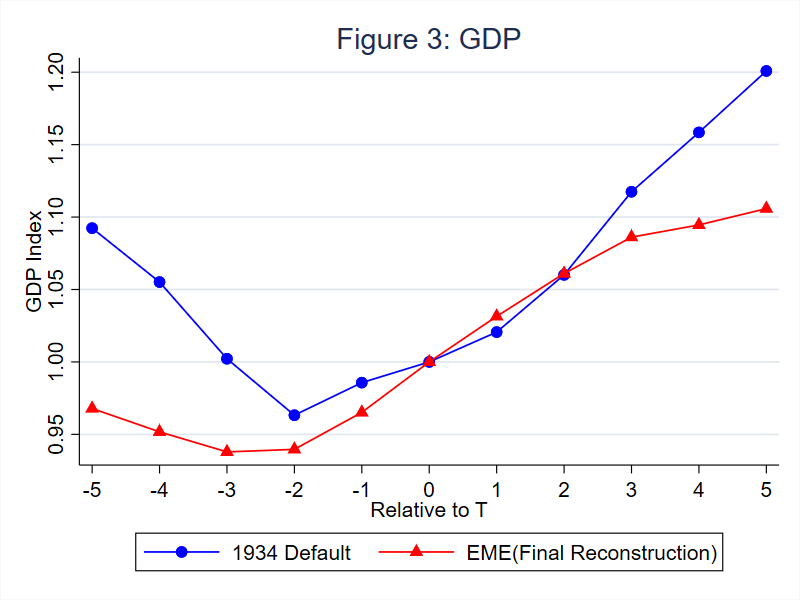
\includegraphics[width=\textwidth]{figures/Figure3_GDP_Comparison.png}
        \caption{Real per capita GDP around debt relief events (exit from default) in middle- to high-
income emerging markets (1978-2010) and advanced economies (1934).}
        \label{fig:3}
    \end{subfigure}
    \hfill
    \begin{subfigure}[b]{0.48\textwidth}
        \centering
        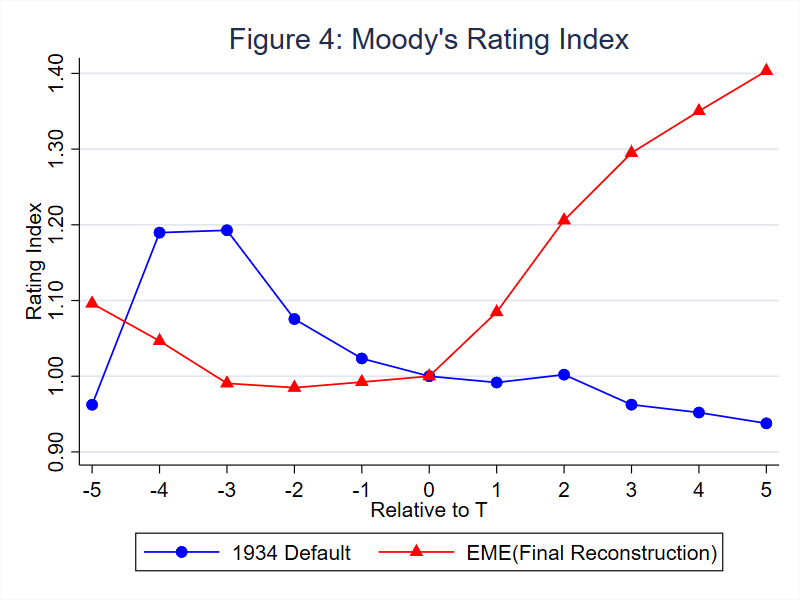
\includegraphics[width=\textwidth]{figures/Figure4_Rating_Comparison.png}
        \caption{Total external debt to GDP (in \%) around debt relief events (exit from default) in
        middle- to high-income emerging markets (1978-2010) and advanced economies (1934).}
        \label{fig:4}
    \end{subfigure}
\end{figure}

\begin{figure}[ht!]
    \centering
    \begin{subfigure}[b]{0.48\textwidth}
        \centering
        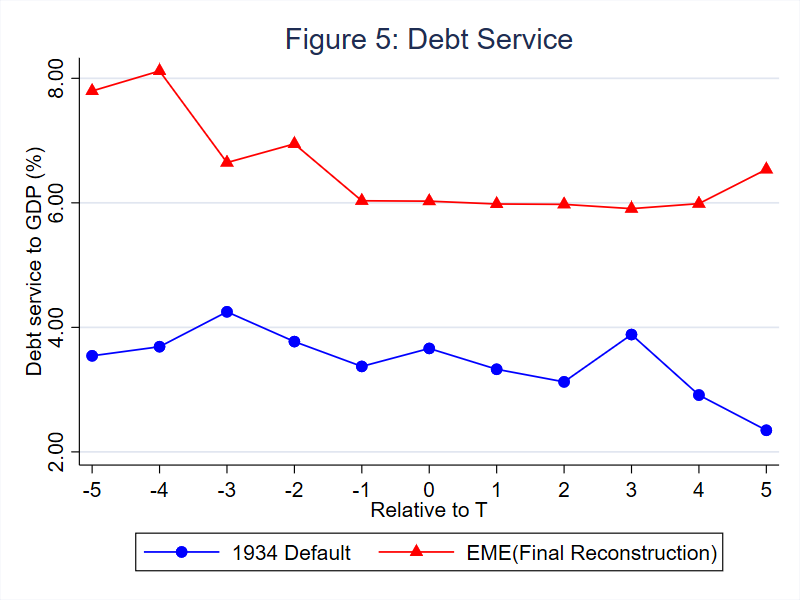
\includegraphics[width=\textwidth]{figures/Figure5_DebtService_Comparison.png}
        \caption{Total debt service to GDP (in \%) around debt relief events (exit from default) in
        middle- to high-income emerging markets (1978-2010) and advanced economies (1934).}
        \label{fig:5}
    \end{subfigure}
    \hfill
    \begin{subfigure}[b]{0.48\textwidth}
        \centering
        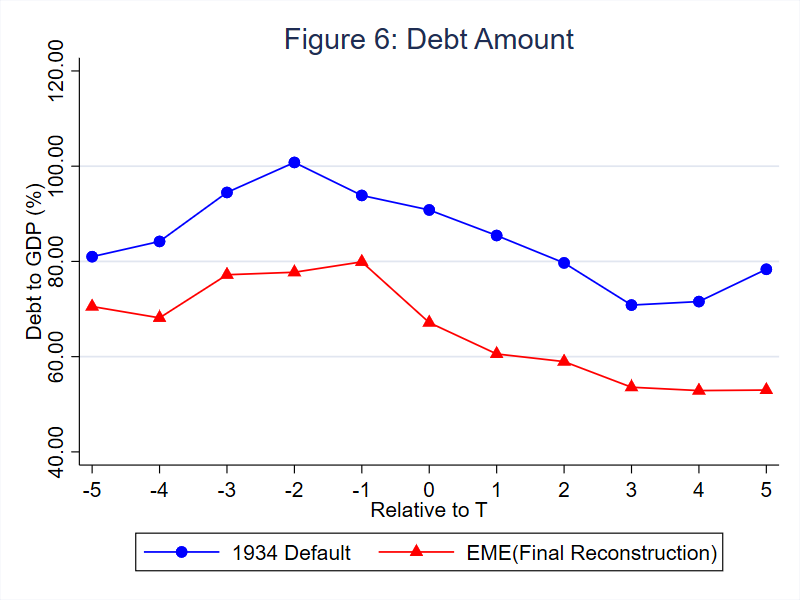
\includegraphics[width=\textwidth]{figures/Figure6_DebtStock_Comparison.png}
        \caption{Debt to GDP (in \%) around debt relief events (exit from default) in middle- to high-
income emerging markets (1978-2010) and advanced economies (1934).}
        \label{fig:6}
    \end{subfigure}
\end{figure}

\subsection{Parallel trend test}
We found out that the author only used the data to make descriptive analysis, but did not
use the data to make a parallel trend test. So, we work on the parallel trend test ourselves, and the results are as below.

To see the results more easily, we write into a matrix:
\begin{table}[ht!]
\centering
\begin{tabular}{lccc}
\toprule
Variable & P‐Value & Pass (5\%) & Pass (10\%) \\
\midrule
GDP\_Growth\_1934\_l   & 0.52529567 & 1 & 1 \\
GDP\_Growth\_1934\_e   & 0.94559858 & 1 & 1 \\
Ratings\_1934          & 0.04996219 & 0 & 0 \\
DebtServ\_1934\_l      & 0.13978740 & 1 & 1 \\
DebtServ\_1934\_e      & 0.51155188 & 1 & 1 \\
Debt\_GDP\_1934\_l     & 0.12776463 & 1 & 1 \\
Debt\_GDP\_1934\_e     & 0.25006164 & 1 & 1 \\
ExtDebt\_1934          & 0.06999843 & 1 & 0 \\
\midrule
GDP\_Growth\_1931\_l   & 0.57373095 & 1 & 1 \\
GDP\_Growth\_1931\_e   & 0.23592213 & 1 & 1 \\
Ratings\_1931          & 0.41062027 & 1 & 1 \\
DebtServ\_1931\_l      & 0.28772333 & 1 & 1 \\
DebtServ\_1931\_e      & 0.39504800 & 1 & 1 \\
Debt\_GDP\_1931\_l     & 0.01403155 & 0 & 0 \\
Debt\_GDP\_1931\_e     & 0.07416818 & 1 & 0 \\
ExtDebt\_1931          & 0.01362215 & 0 & 0 \\
\bottomrule
\end{tabular}
\caption{P-values and pass/fail indicators at 5\% and 10\% levels}
\label{tab:pass_tests}
\end{table}


From this table, we could see that main results are available, most variables pass the test,
only two variables failed, which we need to interpret with caution:
\begin{itemize}
    \item Credit rating results for 1934
    \item Debt/GDP ratio and external debt/GDP ratio results for 1931
\end{itemize}

\begin{figure}[ht!]
    \centering
    \begin{subfigure}[b]{0.48\textwidth}
        \centering
        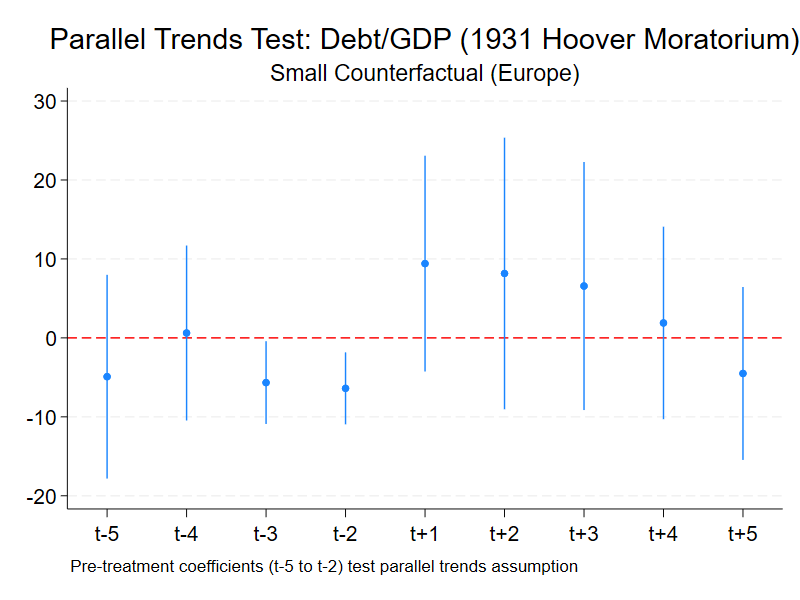
\includegraphics[width=\textwidth]{figures/PT_Debt_1931_Small.png}
        \caption{Parallel Trend Test 1}
        \label{fig:pt1}
    \end{subfigure}
    \hfill
    \begin{subfigure}[b]{0.48\textwidth}
        \centering
        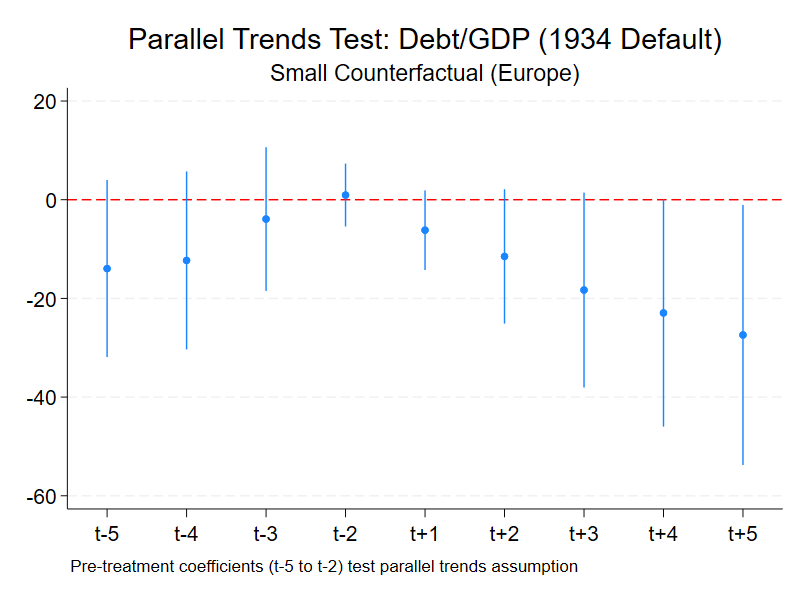
\includegraphics[width=\textwidth]{figures/PT_Debt_1934_Small.png}
        \caption{Parallel Trend Test 2}
        \label{fig:pt2}
    \end{subfigure}
    \\[1em]
    \begin{subfigure}[b]{0.48\textwidth}
        \centering
        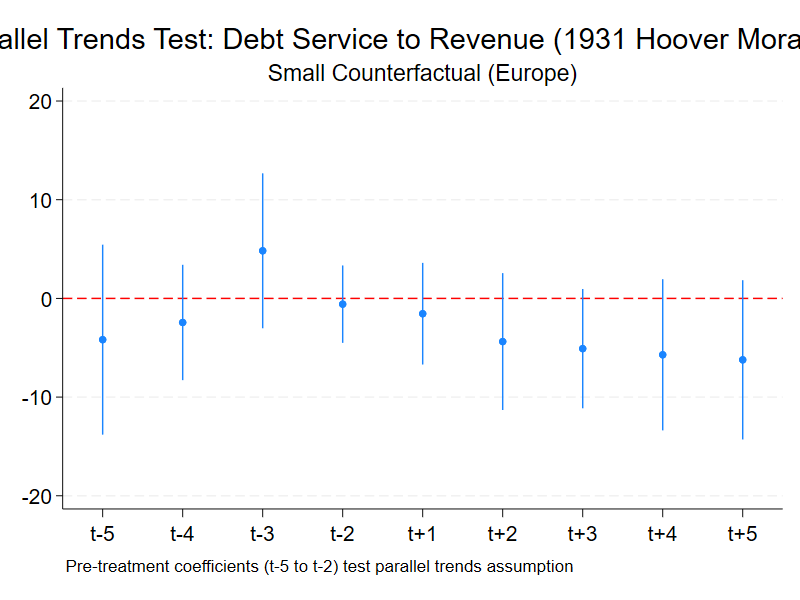
\includegraphics[width=\textwidth]{figures/PT_DebtServ_1931_Small.png}
        \caption{Parallel Trend Test 3}
        \label{fig:pt3}
    \end{subfigure}
    \hfill
    \begin{subfigure}[b]{0.48\textwidth}
        \centering
        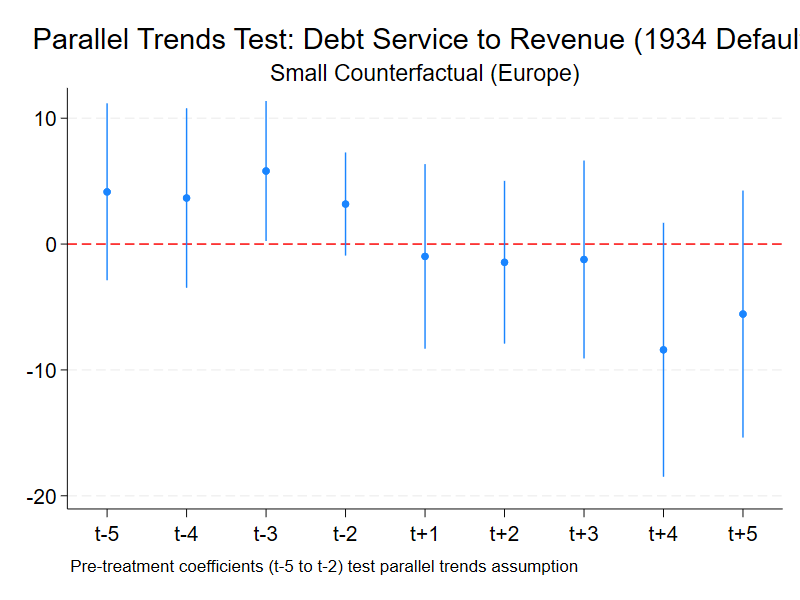
\includegraphics[width=\textwidth]{figures/PT_DebtServ_1934_Small.png}
        \caption{Parallel Trend Test 4}
        \label{fig:pt4}
    \end{subfigure}
    \\[1em]
    \begin{subfigure}[b]{0.48\textwidth}
        \centering
        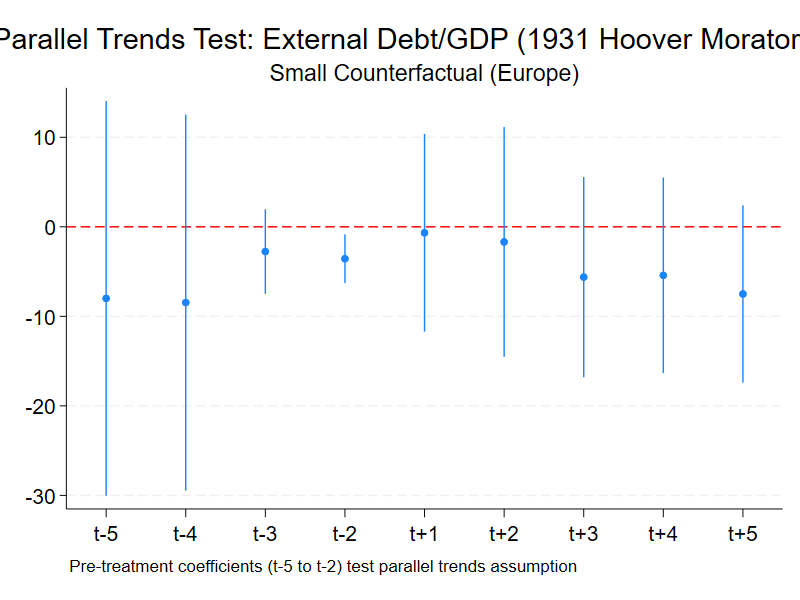
\includegraphics[width=\textwidth]{figures/PT_ExtDebt_1931.png}
        \caption{Parallel Trend Test 5}
        \label{fig:pt5}
    \end{subfigure}
    \hfill
    \begin{subfigure}[b]{0.48\textwidth}
        \centering
        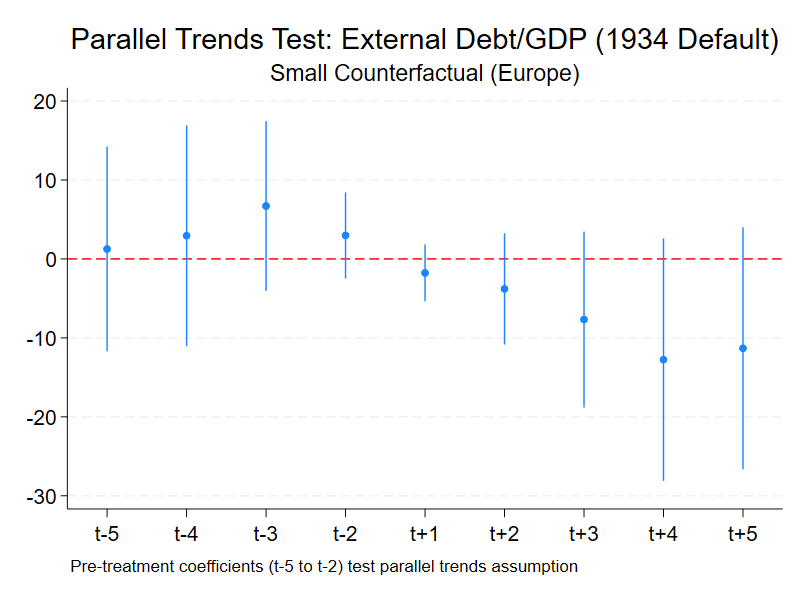
\includegraphics[width=\textwidth]{figures/PT_ExtDebt_1934.png}
        \caption{Parallel Trend Test 6}
        \label{fig:pt6}
    \end{subfigure}
    \\[1em]
    \begin{subfigure}[b]{0.48\textwidth}
        \centering
        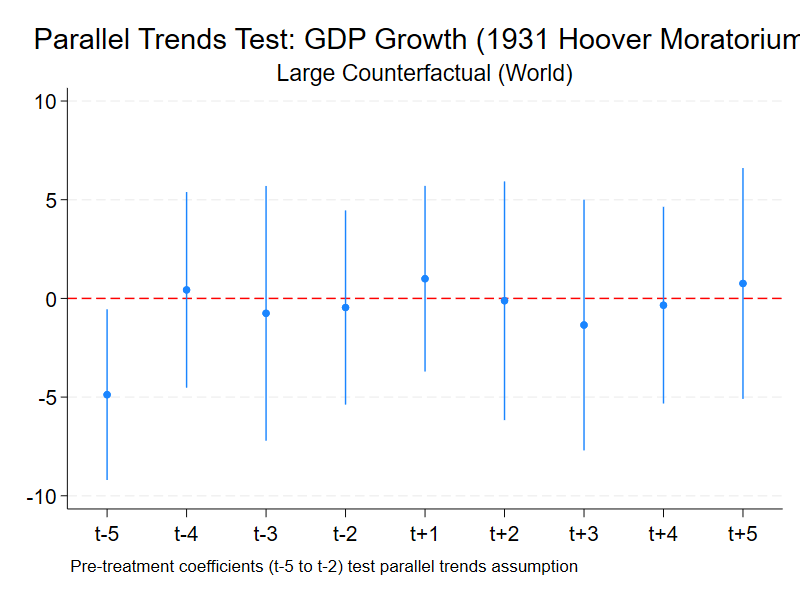
\includegraphics[width=\textwidth]{figures/PT_GDP_1931_Large.png}
        \caption{Parallel Trend Test 7}
        \label{fig:pt7}
    \end{subfigure}
    \hfill
    \begin{subfigure}[b]{0.48\textwidth}
        \centering
        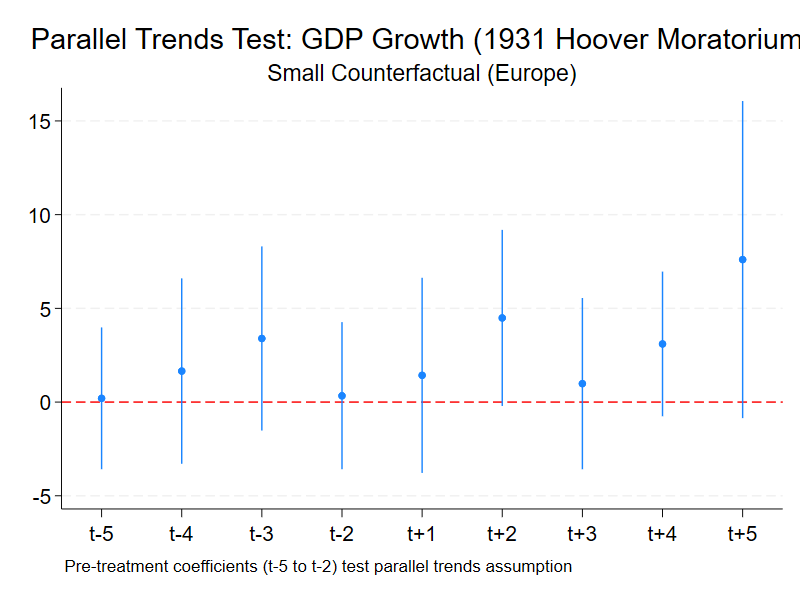
\includegraphics[width=\textwidth]{figures/PT_GDP_1931_Small.png}
        \caption{Parallel Trend Test 8}
        \label{fig:pt8}
    \end{subfigure}
    \caption{Parallel trend test results for different country samples and variables}
    \label{fig:parallel_trends}
\end{figure}

\begin{figure}[ht!]
    \centering
    \begin{subfigure}[b]{0.48\textwidth}
        \centering
        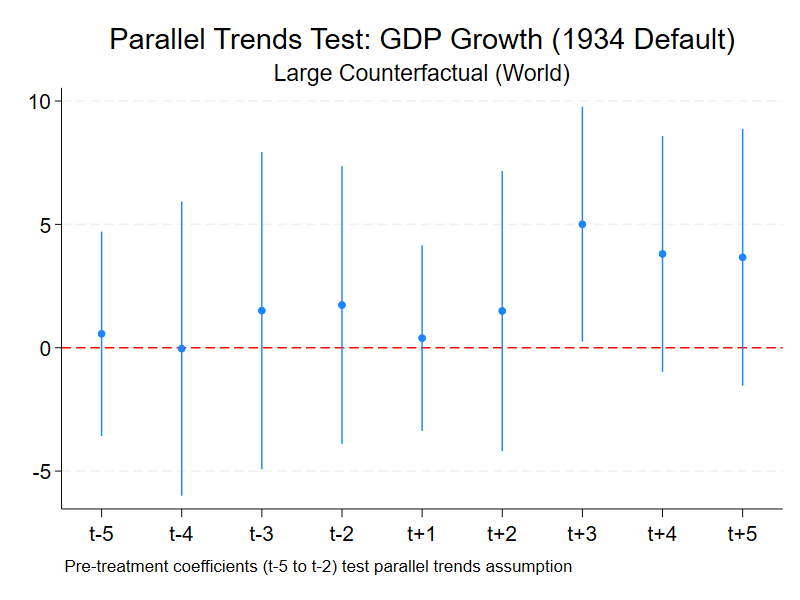
\includegraphics[width=\textwidth]{figures/PT_GDP_1934_Large.png}
        \caption{Parallel Trend Test 9}
        \label{fig:pt9}
    \end{subfigure}
    \hfill
    \begin{subfigure}[b]{0.48\textwidth}
        \centering
        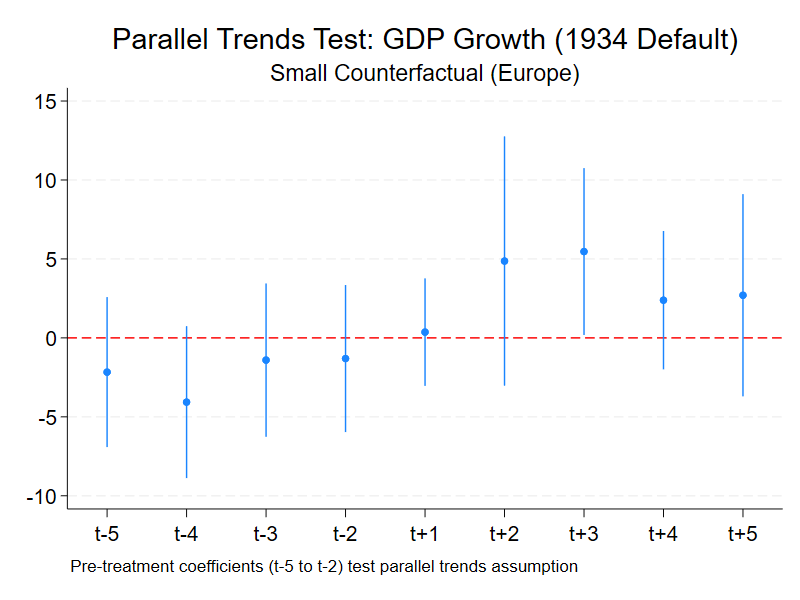
\includegraphics[width=\textwidth]{figures/PT_GDP_1934_Small.png}
        \caption{Parallel Trend Test 10}
        \label{fig:pt10}
    \end{subfigure}
    \hfill
    \begin{subfigure}[b]{0.48\textwidth}
        \centering
        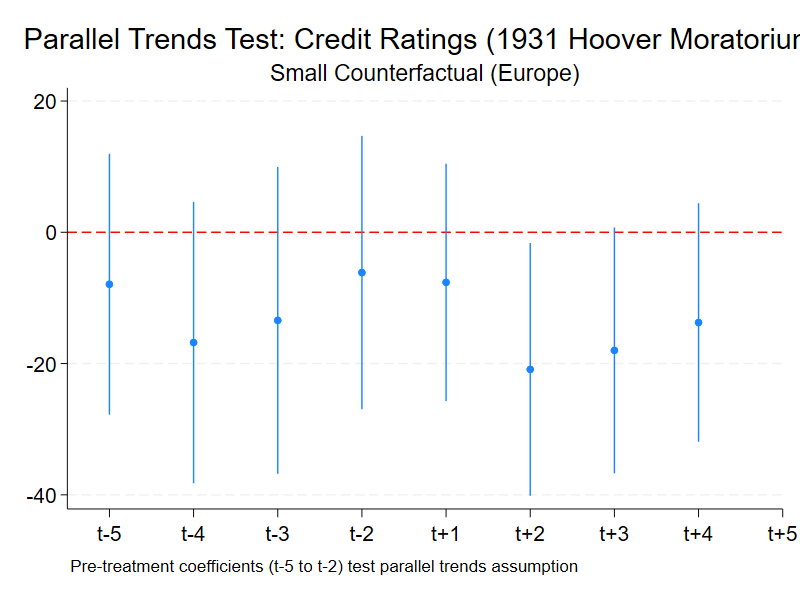
\includegraphics[width=\textwidth]{figures/PT_Ratings_1931.png}
        \caption{Parallel Trend Test 11}
        \label{fig:pt11}
    \end{subfigure}
    \hfill
    \begin{subfigure}[b]{0.48\textwidth}
        \centering
        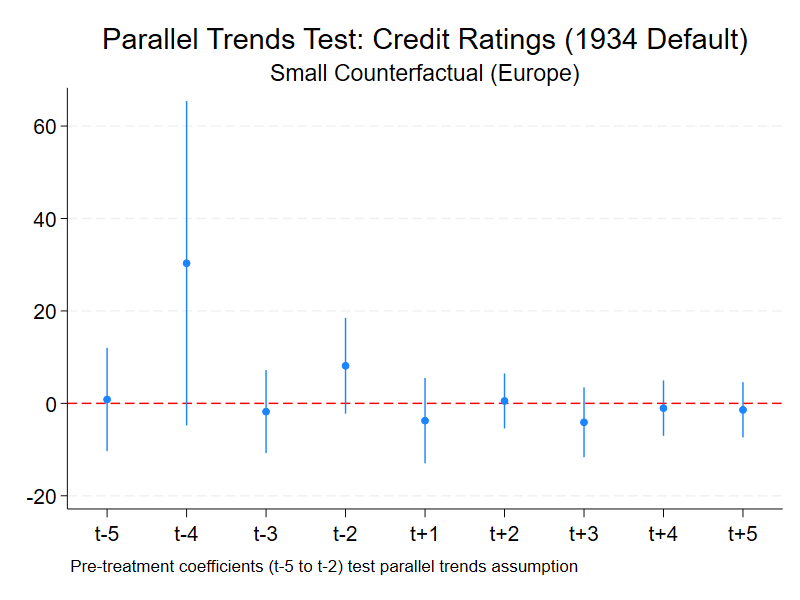
\includegraphics[width=\textwidth]{figures/PT_Ratings_1934.png}
        \caption{Parallel Trend Test 12}
        \label{fig:pt12}
    \end{subfigure}
    \caption{Parallel trend test results for different country samples and variables}
    \label{fig:parallel_trends2}
\end{figure}

\subsection{DID Analysis}

The Brady target group includes all middle-income
EMs with a Brady deal, namely Argentina, Brazil, Bulgaria, Costa Rica, Dominican
Republic, Ecuador, Jordan, Mexico, Panama, Peru, Poland, Uruguay, and Venezuela.
The Baker country sample is the same, plus Chile, which was a target country in the
mid-1980s, but were not part of the “Brady bunch”.

The baseline counterfactual includes all middle- and high-income countries(regions)
that did not default nor received debt relief in this period and for which we have data,
namely China, Colombia, Czech Republic, Egypt, Hungary, India, Israel, Malaysia,
Mauritius, Singapore, South Korea, Taiwan, Thailand, and Turkey.

We start with the Hoover Moratorium of 1931 and take a preliminary view of the
data.

\begin{figure}[ht!]
    \centering
    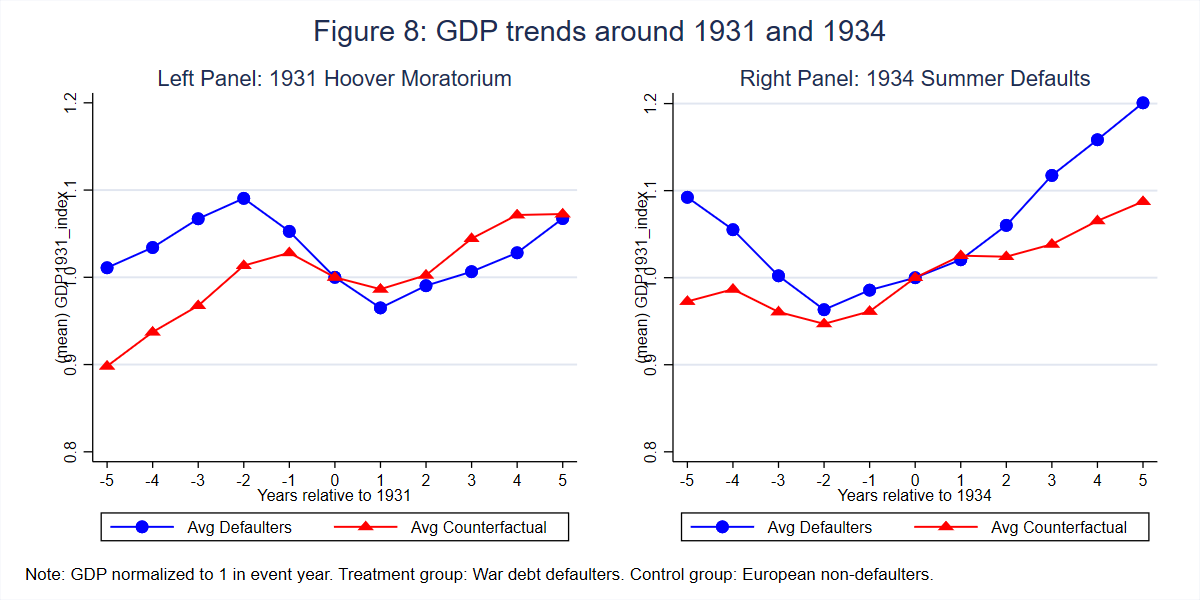
\includegraphics[width=0.95\textwidth]{figures/Figure8_GDP_trends_1931_1934.png}
    \caption{GDP trends around 1931 and 1934}
    \label{fig:8}
\end{figure}

\begin{figure}[ht!]
    \centering
    \begin{subfigure}[b]{0.48\textwidth}
        \centering
        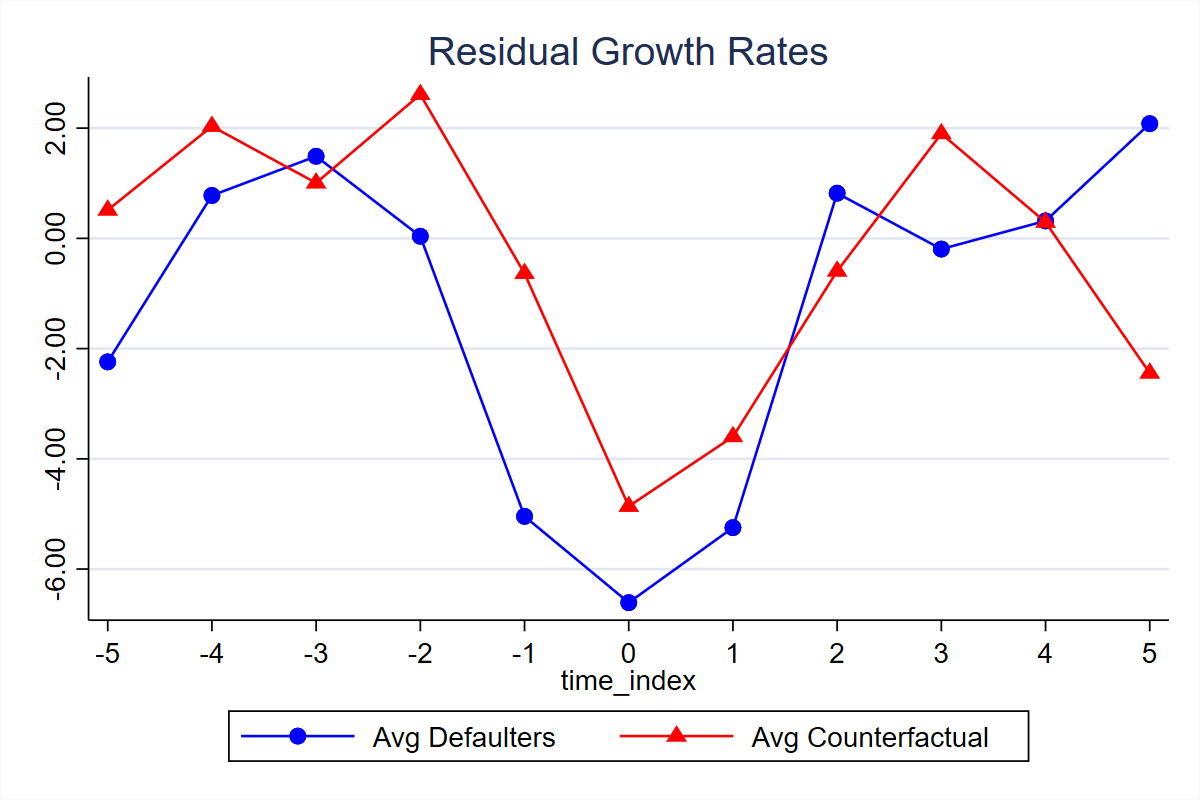
\includegraphics[width=\textwidth]{figures/figc5_a.png}
        \caption{Residual GDP Growth}
        \label{fig:c5a}
    \end{subfigure}
    \hfill
    \begin{subfigure}[b]{0.48\textwidth}
        \centering
        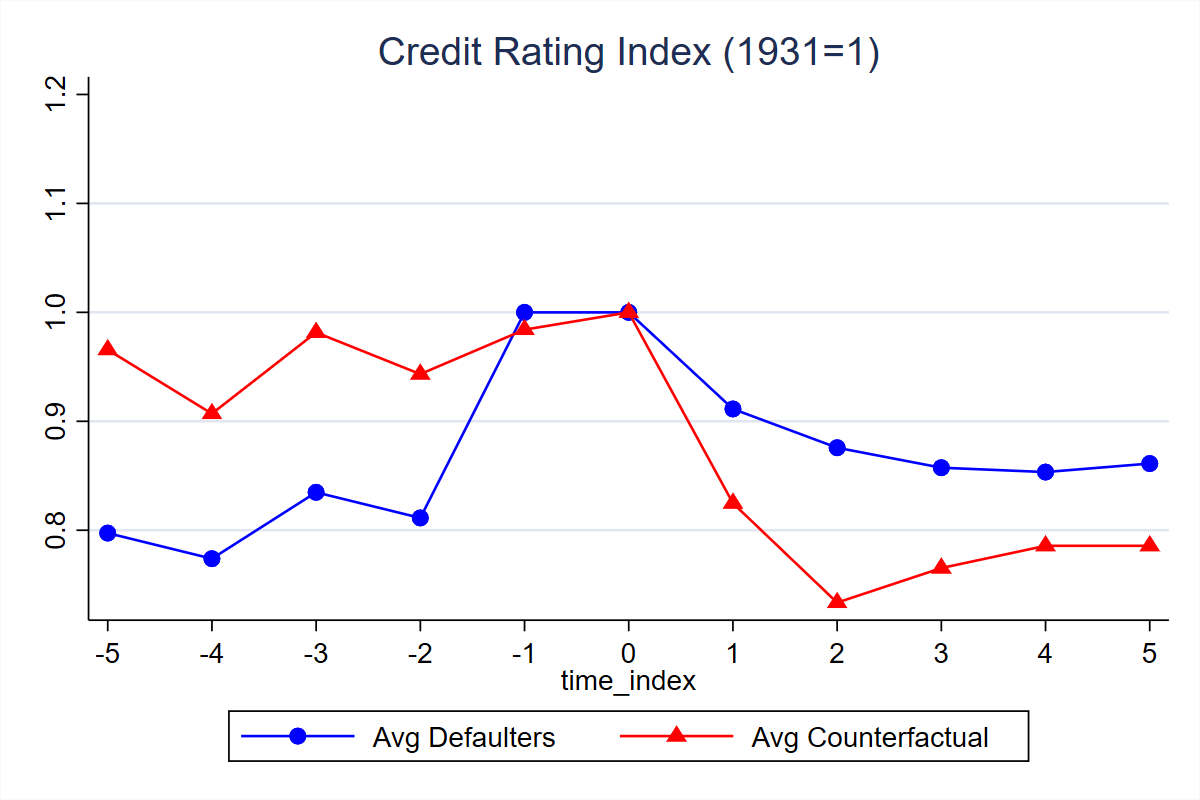
\includegraphics[width=\textwidth]{figures/figc5_b.png}
        \caption{Credit Ratings}
        \label{fig:c5b}
    \end{subfigure}
    \\[1em]
    \begin{subfigure}[b]{0.48\textwidth}
        \centering
        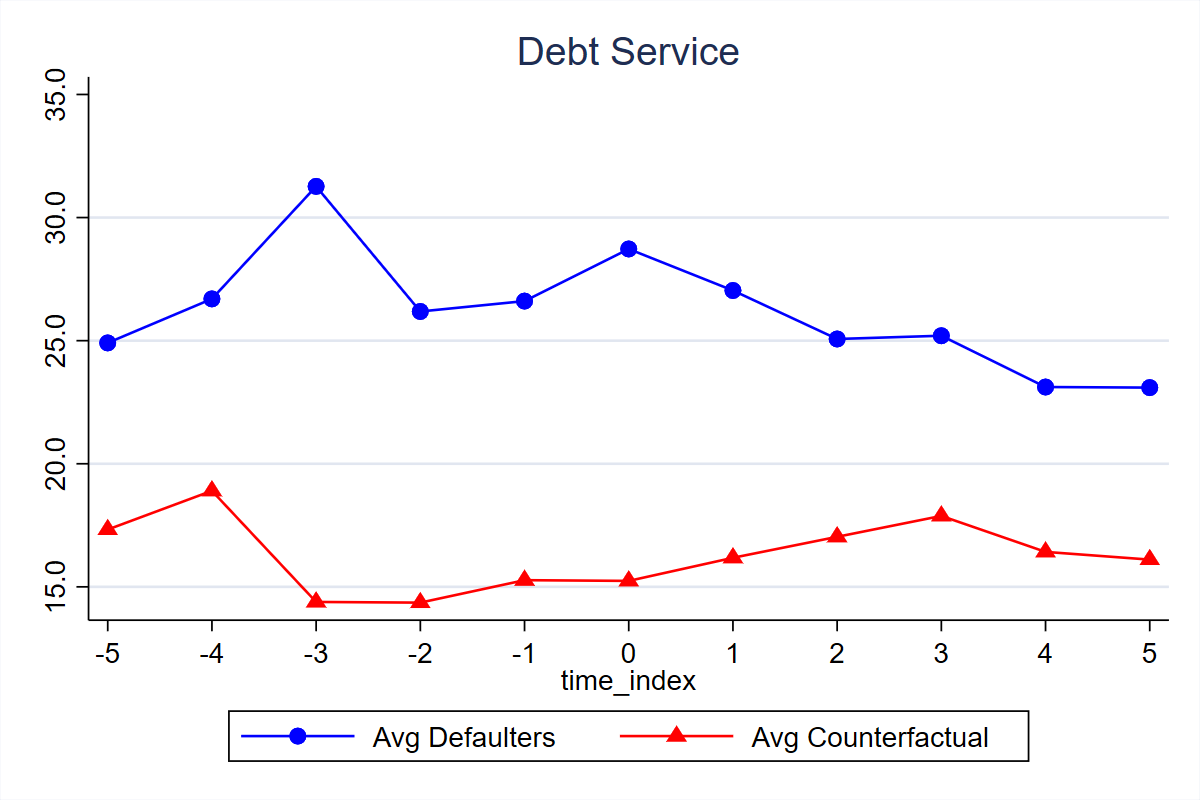
\includegraphics[width=\textwidth]{figures/figc5_c.png}
        \caption{Debt Service to Revenue}
        \label{fig:c5c}
    \end{subfigure}
    \hfill
    \begin{subfigure}[b]{0.48\textwidth}
        \centering
        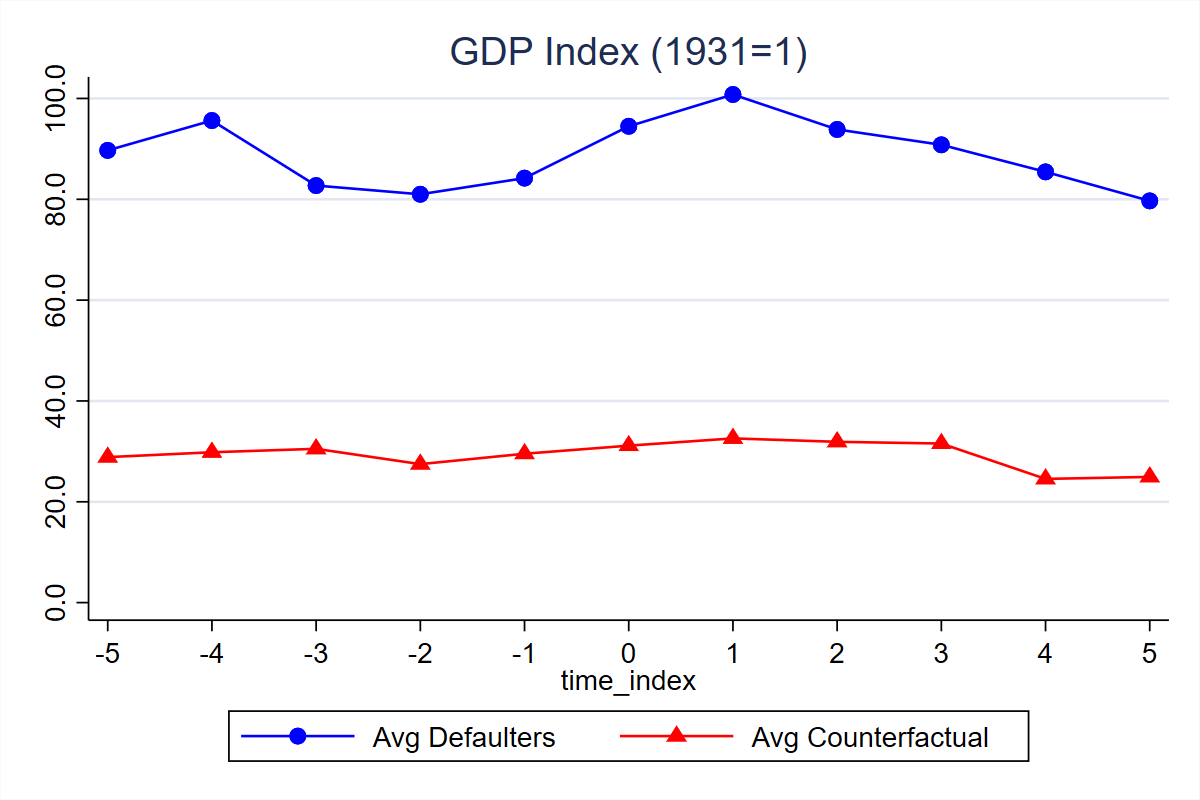
\includegraphics[width=\textwidth]{figures/figc5_d.png}
        \caption{Debt to GDP}
        \label{fig:c5d}
    \end{subfigure}
    \caption{Economic indicators comparison between treatment and control groups}
    \label{fig:c5}
\end{figure}

The figures compare the development of our main economic indicators for treatment and control groups,
where the control groups is our baseline sample of European non-defaulters.
Figure 8 (left panel) shows that the growth performance of the treatment group is significantly worse
than that of the counterfactual around 1931. 

Panel B: country
heterogeneity by showing residuals from a regression of annual real p.c. growth on a
constant and country-specific dummies. Residual growth declines markedly for both
groups prior to 1931 and recovers strongly afterwards, but there is no evidence that
treatment countries perform better than the counterfactual.

Panel C: The picture is similarly
bleak with regard to Moody's credit ratings, which decline across the board after 1931,
with no notable difference between the two groups. 

Panel D: Similarly, the debt/GDP
level does not decline significantly more for the target countries. Only the
debt servicing burden improves, as payments to revenue drop relatively more than
those countries not receiving relief.

\subsection{Results of DID}
The results are more notable for the 1934 debt relief spell. Table 4 indicates that
real per capita growth is 4.7 percentage points higher for treated countries in the post-
1934 period, with a highly significant coefficient (column (1)). Moreover, the debt
levels decrease significantly (columns (6) and (8)), compared to the counterfactual on
European non-defaulters. We find no significant coefficient for debt servicing (column
(4)) and a highly significant negative coefficient for ratings. These results, however,
are rather sensitive to the choice of counterfactual, as can be seen in columns (2),
(5), and (7), which use the “World” counterfactual including European, Asian, and
South American countries. The treatment coefficient for debt servicing becomes highly
significant and large, while the coefficient for debt/GDP turns insignificant. Notably,
however, the growth coefficient remains large and significant across all counterfactuals
chosen, albeit sometimes only at the 10\% level.

\begin{sidewaystable}[ht!]\centering
\def\sym#1{\ifmmode^{#1}\else\(^{#1}\)\fi}
\caption{Table 3: 1931 Hoover Moratorium - Difference-in-Difference Analysis}
\renewcommand{\arraystretch}{1.2} % 增加行距
\begin{tabular*}{\textwidth}{@{\hskip\tabcolsep\extracolsep\fill}p{3.75cm}*{8}{>{\centering\arraybackslash}p{2.25cm}}}
\hline\hline
            &(1)&(2)&(3)&(4)&(5)&(6)&(7)&(8)\\
            &\parbox{2.25cm}{\centering Growth, real p.c.\\Small (Europe)}&\parbox{2.25cm}{\centering Growth, real p.c.\\Large (World)}&\parbox{2.25cm}{\centering Credit Ratings (change)\\Small (Europe)}&\parbox{2.25cm}{\centering Debt Service to Revenue\\Small (Europe)}&\parbox{2.25cm}{\centering Debt Service to Revenue\\Large (World)}&\parbox{2.25cm}{\centering Total Public Debt/GDP\\Small (Europe)}&\parbox{2.25cm}{\centering Total Public Debt/GDP\\Large (World)}&\parbox{2.25cm}{\centering External Debt/GDP\\Small (Europe)}\\
\hline
\parbox{3cm}{\raggedright Post-intervention dummy (after 1931)}&  $4.922^{**}$  &  $8.329^{***}$  &  $3.752$  &  $-1.064$  &  $-3.882^{**}$&  $-10.011^{*}$  &  $-7.900^{*}$ &  $-9.086^{**}$  \\
            &  $(2.335)$  &  $(1.724)$ & $(3.377)$   &  $(1.880)$   &  $(1.854)$  &  $(4.854)$  &  $(4.240)$  & $(3.687)$   \\
[0.5em]
\parbox{3cm}{\raggedright Treatment (war debt moratorium) $\times$ post-intervention dummy}&  $2.598^{*}$&  $0.862$  &  $-5.655$&  $-4.310^{*}$  &  $-3.390$   &  $7.312$ &  $3.822$   &  $-0.508$ \\
            &  $(1.360)$   &  $(1.333)$   &  $(4.202)$   &  $(2.392)$   &  $(2.335)$   &  $(6.936)$   &  $(6.899)$   &  $(5.610)$   \\
[0.5em]
Constant    &  $-4.072^{***}$&  $-4.489^{***}$&  $0.906$   &  $24.360^{***}$&  $23.973^{***}$&  $69.849^{***}$&  $61.471^{***}$&  $32.183^{***}$\\
            &  $(0.839)$   &  $(1.160)$   &  $(2.058)$   &  $(1.215)$   &  $(0.990)$   &  $(1.872)$   &  $(1.695)$   &  $(2.174)$   \\
\hline
Observations&         237   &         373   &         230   &         223   &         326   &         172   &         248   &         167   \\
Adjusted R² &       0.237   &       0.206   &       0.185   &       0.043   &       0.062   &       0.166   &       0.199   &       0.007   \\
\hline\hline
\multicolumn{9}{p{0.95\textwidth}}{\footnotesize \textbf{Notes:} This table reports difference-in-difference estimates of the effect of the 1931 Hoover Moratorium on various economic outcomes. Treatment group consists of 18 countries that received war debt relief. Small counterfactual includes European non-defaulters; Large counterfactual adds Latin American and other countries. All regressions include country and year fixed effects. Standard errors clustered at country level in parentheses. $^*$ p<0.10, $^{**}$ p<0.05, $^{***}$ p<0.01}\\
\end{tabular*}
\end{sidewaystable}


When we are working on Table3, we found out a bug:
the data of column (3), (4), (5) might be in the wrong order, the correct order of data should be (5), (3), (4).

Also, the post-intervention dummy (after 1931) is very different from authors' result, we also tried to drop the year fixed effect, but the result is still different.
(We tried to run authors' original code, and the results are the same as what we get, not what's in the table of this paper.)

According to the authors based on their result, `The only $\beta_2$ coefficients that are marginally significant are those of GDP and of credit ratings',
but as we could see from our table, only credit ratings and debt service to revenue in treated countries are insignificant.

\begin{figure}[ht!]
    \centering
    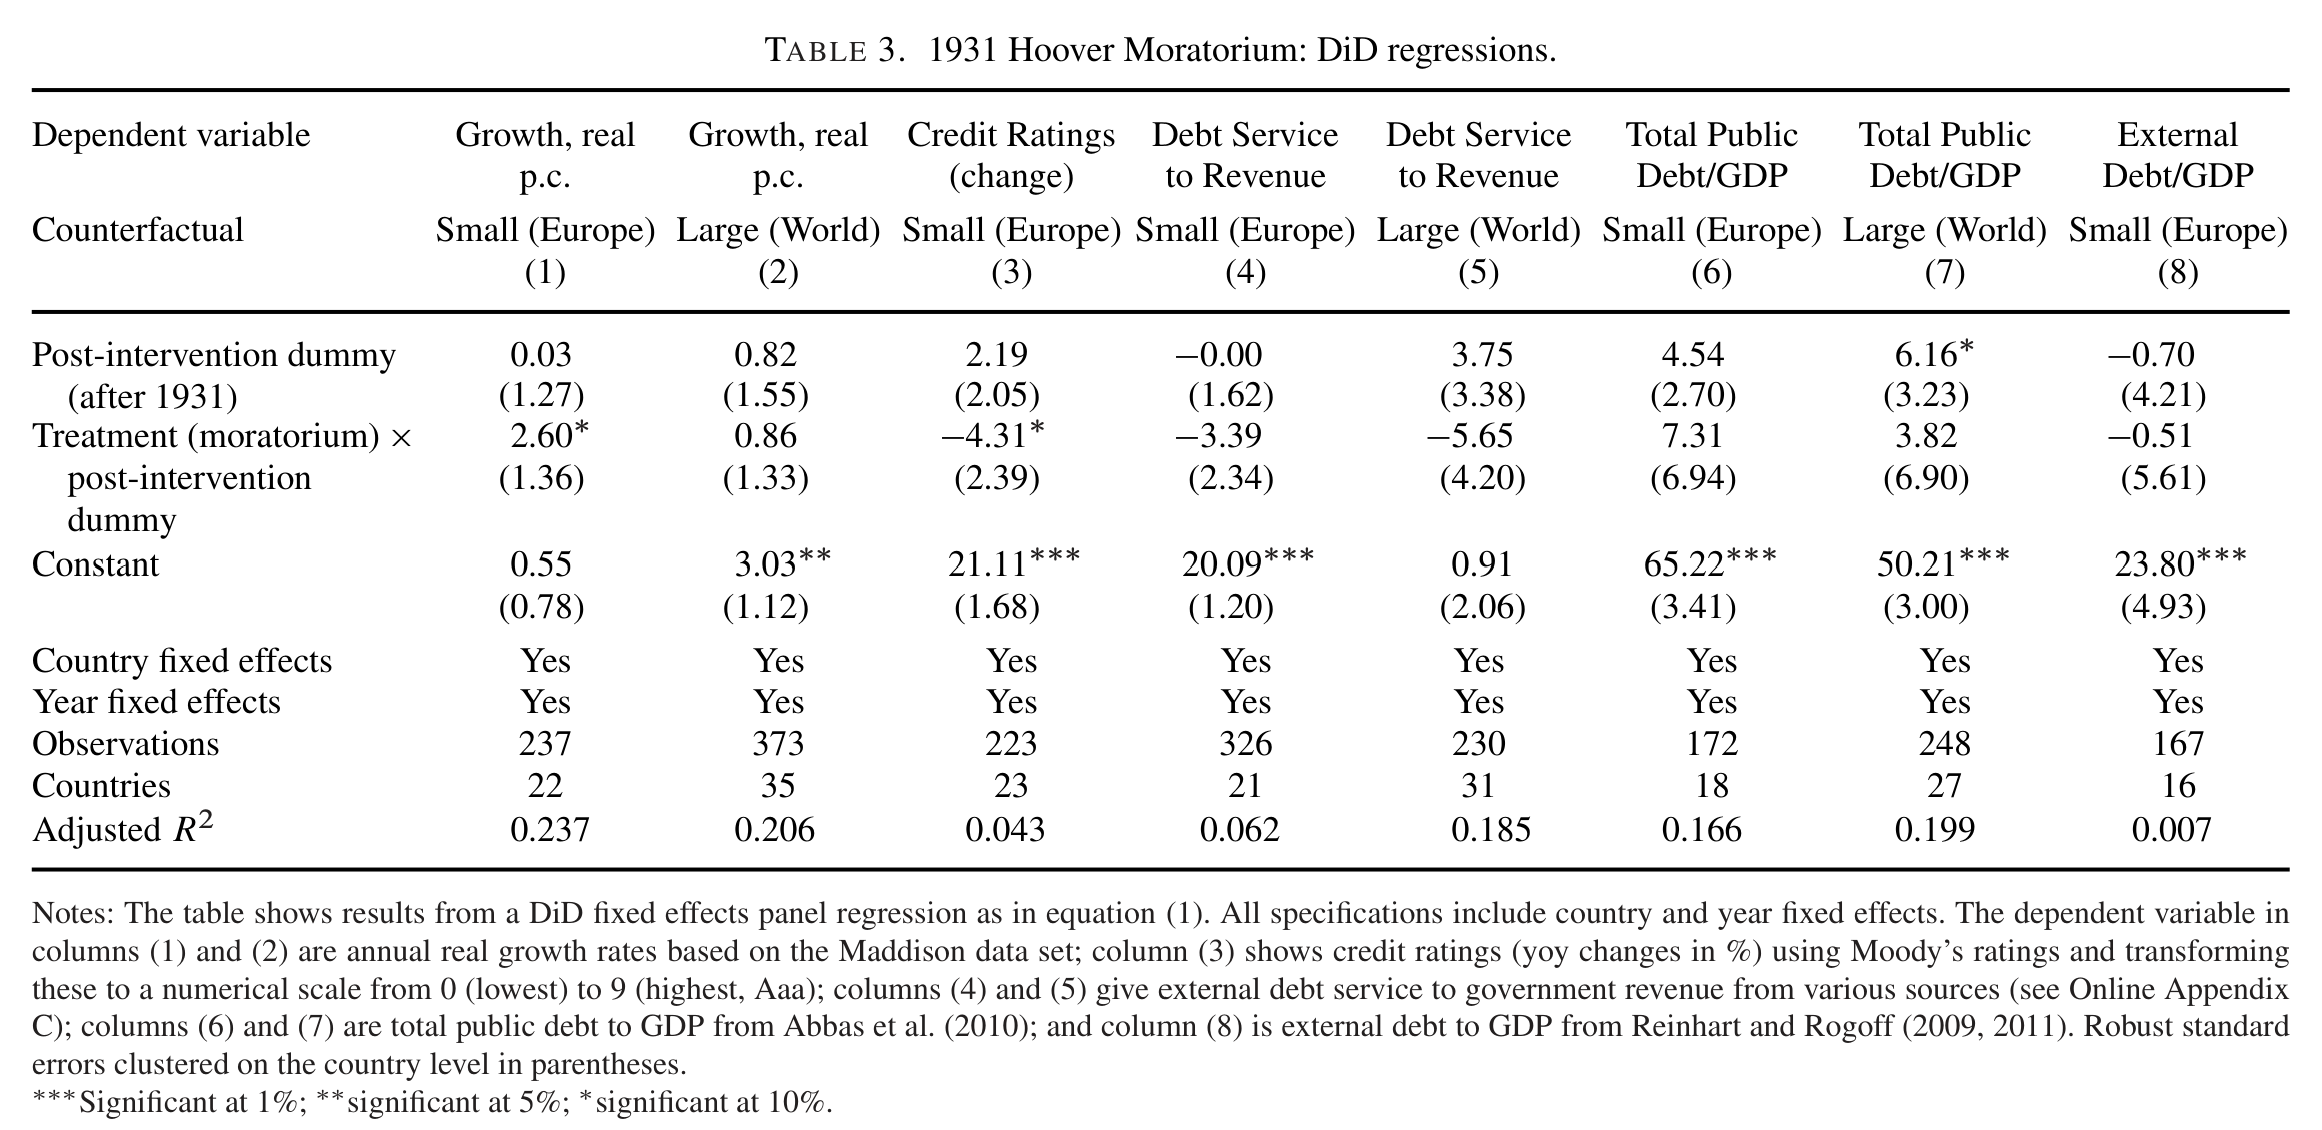
\includegraphics[width=0.95\textwidth]{figures/table3_original.png}
    \caption{Table 3 Original}
    \label{fig:table3_original}
\end{figure}

\begin{figure}[ht!]
    \centering
    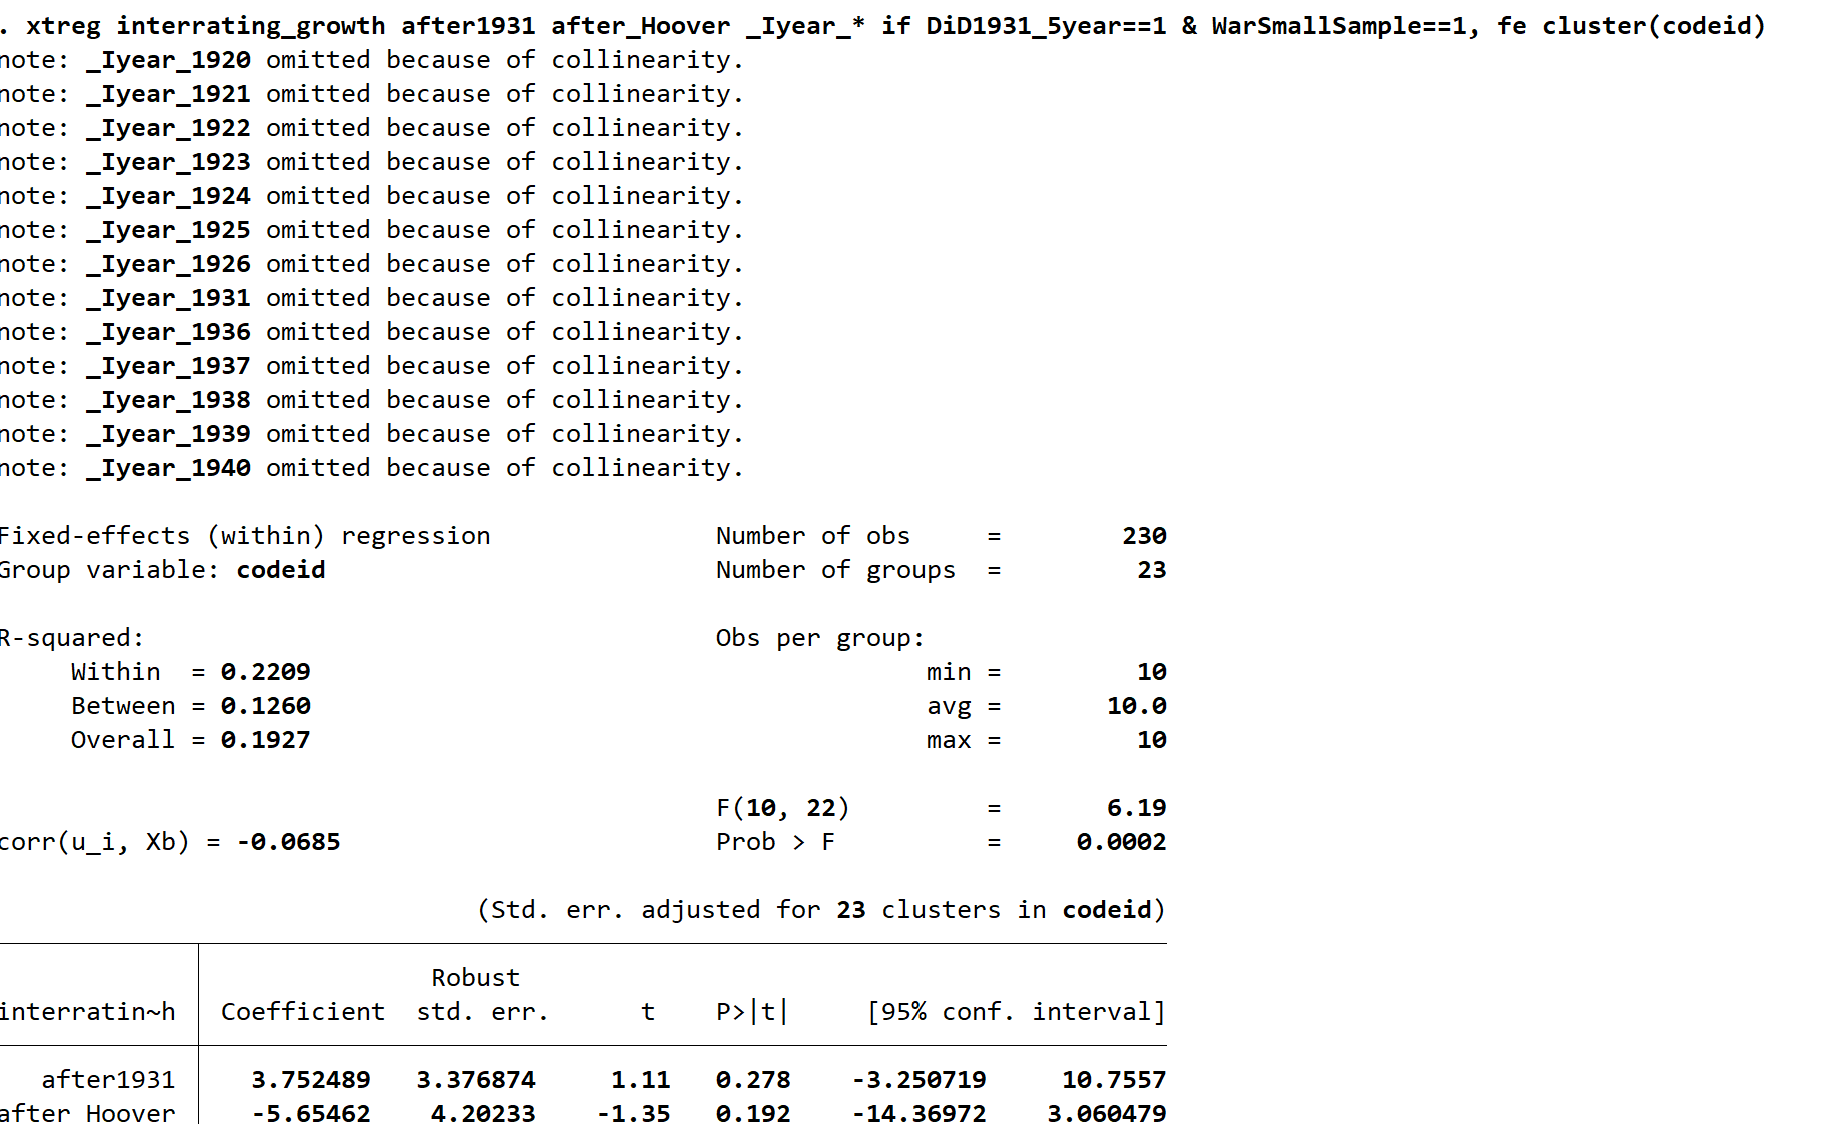
\includegraphics[width=0.95\textwidth]{figures/col3_tab3_stata.png}
    \caption{Table 3 Col 3}
    \label{fig:table3_col3}
\end{figure}

\begin{figure}[ht!]
    \centering
    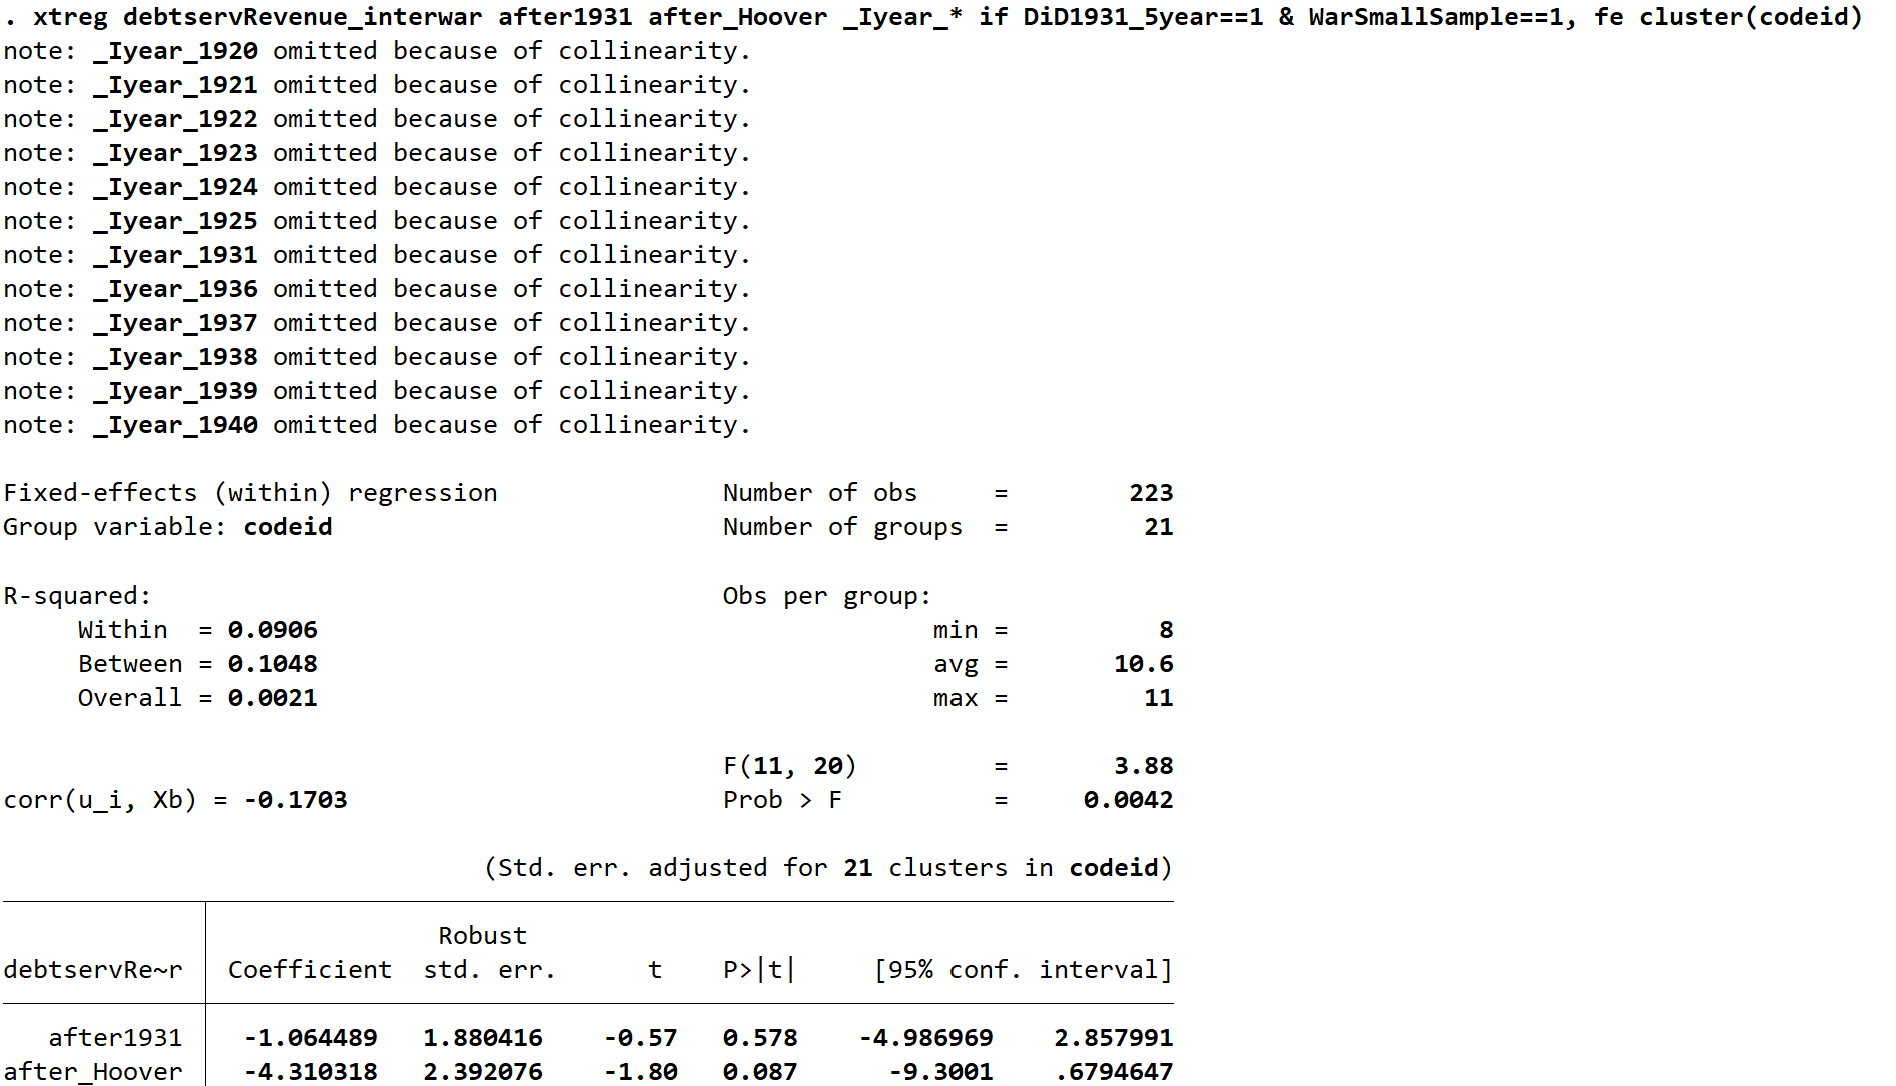
\includegraphics[width=0.95\textwidth]{figures/col4_tab3_stata.png}
    \caption{Table 3 Col 4}
    \label{fig:table3_col4}
\end{figure}

\begin{sidewaystable}[ht!]\centering
\def\sym#1{\ifmmode^{#1}\else\(^{#1}\)\fi}
\caption{Table 4: 1934 Summer Defaults - Difference-in-Difference Analysis}
\renewcommand{\arraystretch}{1.2} % 增加行距
\begin{tabular*}{\textwidth}{@{\hskip\tabcolsep\extracolsep\fill}p{3.75cm}*{8}{>{\centering\arraybackslash}p{2.25cm}}}
\hline\hline
            &(1)&(2)&(3)&(4)&(5)&(6)&(7)&(8)\\
            &\parbox{2.25cm}{\centering Growth, real p.c.\\Small (Europe)}&\parbox{2.25cm}{\centering Growth, real p.c.\\Large (World)}&\parbox{2.25cm}{\centering Credit Ratings (change)\\Small (Europe)}&\parbox{2.25cm}{\centering Debt Service to Revenue\\Small (Europe)}&\parbox{2.25cm}{\centering Debt Service to Revenue\\Large (World)}&\parbox{2.25cm}{\centering Total Public Debt/GDP\\Small (Europe)}&\parbox{2.25cm}{\centering Total Public Debt/GDP\\Large (World)}&\parbox{2.25cm}{\centering External Debt/GDP\\Small (Europe)}\\
\hline
\parbox{3cm}{\raggedright Post-intervention dummy (after 1934)}&  $-1.905$  &  $-0.772$  &  $4.527^*$  &  $-4.284$  &  $-5.094^{***}$&  $-9.030$  &  $-9.602^{**}$ &  $-3.487$  \\
            &  $(1.320)$  &  $(1.398)$ & $(2.601)$   &  $(2.789)$   &  $(1.837)$  &  $(5.566)$  &  $(4.246)$  & $(3.260)$   \\
[0.5em]
\parbox{3cm}{\raggedright Treatment (debt relief) $\times$ post-intervention dummy}&  $4.658^{***}$&  $2.208^*$  &  $-8.182^{***}$&  $-6.025^*$  &  $-2.744$   &  $-12.206^{**}$ &  $-7.932$   &  $-9.512^{**}$ \\
            &  $(1.437)$   &  $(1.245)$   &  $(2.664)$   &  $(2.989)$   &  $(2.926)$   &  $(5.666)$   &  $(6.180)$   &  $(3.835)$   \\
[0.5em]
Constant    &  $2.399^{***}$&  $3.148^{***}$&  $0.247$   &  $23.094^{***}$&  $21.260^{***}$&  $69.716^{***}$&  $59.571^{***}$&  $25.866^{***}$\\
            &  $(0.643)$   &  $(1.056)$   &  $(2.176)$   &  $(0.950)$   &  $(0.786)$   &  $(3.166)$   &  $(2.382)$   &  $(1.746)$   \\
\hline
Observations&         237   &         378   &         249   &         216   &         324   &         175   &         258   &         162   \\
Adjusted R² &       0.270   &       0.226   &       0.199   &       0.167   &       0.153   &       0.283   &       0.243   &       0.342   \\
\hline\hline
\multicolumn{9}{p{0.95\textwidth}}{\footnotesize \textbf{Notes:} This table reports difference-in-difference estimates of the effect of the 1934 summer debt defaults on various economic outcomes. Treatment group consists of 18 countries that defaulted on war debt. Small counterfactual includes European non-defaulters; Large counterfactual adds Latin American and other countries. All regressions include country and year fixed effects. Standard errors clustered at country level in parentheses. $^*$ p<0.10, $^{**}$ p<0.05, $^{***}$ p<0.01}\\
\end{tabular*}
\end{sidewaystable}




\section{Emerging Markets}

We now study the economic performance before and after the Baker and Brady
initiatives.

\subsection{Parallel Trend Test}

We conduct teh parallel trend test based on the data, and results are as below.
We found out that the author only used the data to make descriptive analysis, but did not
use the data to make a parallel trend test. So, we work on the parallel trend test ourselves, and the results are as below.

To see the results more easily, we write into a matrix:
\begin{table}[ht!]
\centering
\begin{tabular}{lccc}
\toprule
Variable               & P-Value    & Pass (5\%) & Pass (10\%) \\
\midrule
Baker\_GDP         & 0.14110973 & 1          & 1           \\
Baker\_Ratings          & 0.01797839 & 0          & 0           \\
Baker\_DebtSer           & 0.11229144 & 1          & 1           \\
Baker\_Debt           & 0.04972647 & 0          & 0           \\
Baker\_ExtDebt           & 0.80291636 & 1          & 1           \\
\midrule
Brady\_GDP         & 0.05463650 & 1          & 0           \\
Brady\_Ratings           & 0.38826418 & 1          & 1           \\
Brady\_DebtSer           & 0.18770524 & 1          & 1           \\
Brady\_Debt            & 0.30135370 & 1          & 1           \\
Brady\_ExtDebt            & 0.23718979 & 1          & 1           \\
\bottomrule
\end{tabular}
\caption{P-values and pass indicators for Baker and Brady specifications}
\label{tab:baker_brady_tests}
\end{table}

From the marrix we could tell that the main results are also available,
as most variables pass the test. But for the Baker policy, the credit rating and
debt/GDP ratio results failed the test, which we need to interpret with caution.

\begin{figure}[ht!]
    \centering
    \begin{subfigure}[b]{0.48\textwidth}
        \centering
        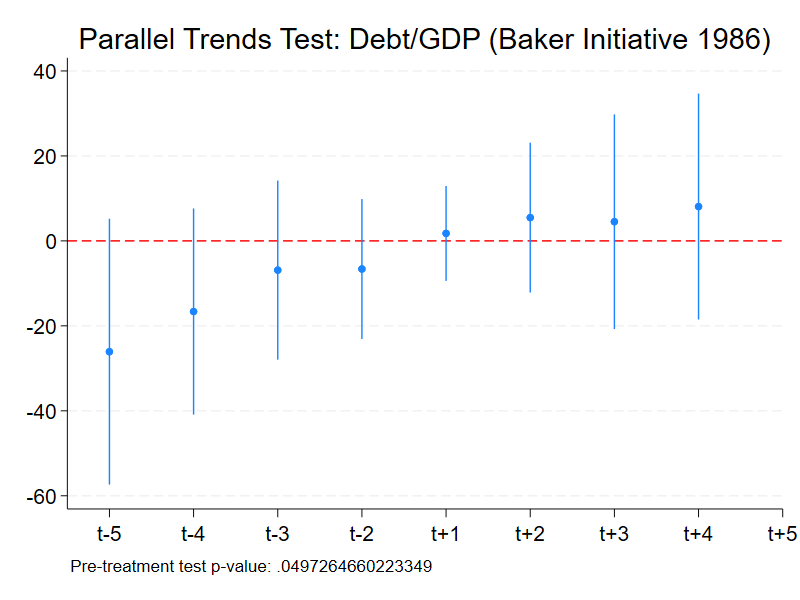
\includegraphics[width=\textwidth]{figures/PT_Baker_Debt.png}
        \caption{Parallel Trend Test 1}
        \label{fig:pt1_eme}
    \end{subfigure}
    \hfill
    \begin{subfigure}[b]{0.48\textwidth}
        \centering
        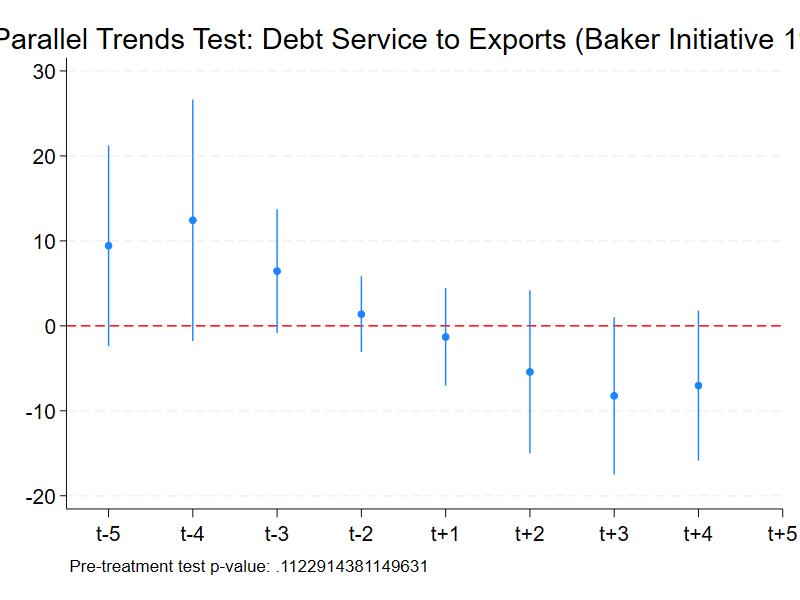
\includegraphics[width=\textwidth]{figures/PT_Baker_DebtServ.png}
        \caption{Parallel Trend Test 2}
        \label{fig:pt2_eme}
    \end{subfigure}
    \\[1em]
    \begin{subfigure}[b]{0.48\textwidth}
        \centering
        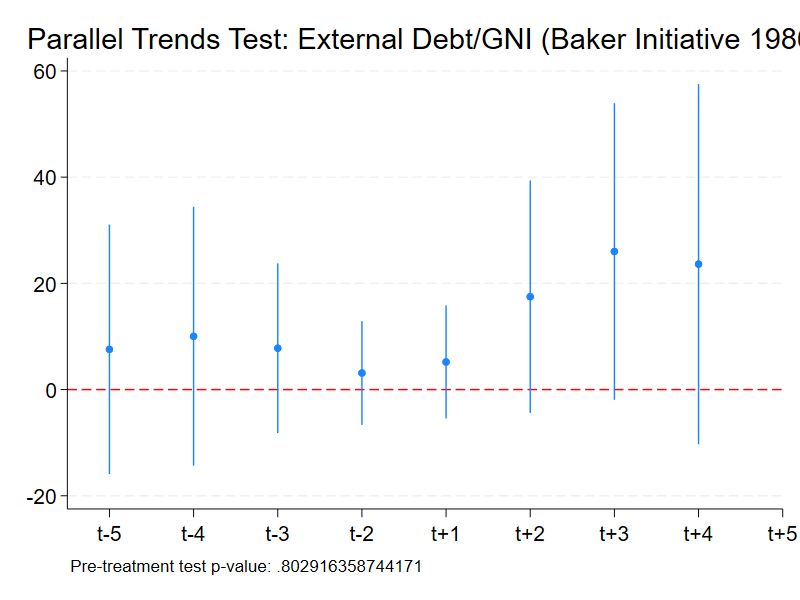
\includegraphics[width=\textwidth]{figures/PT_Baker_ExtDebt.png}
        \caption{Parallel Trend Test 3}
        \label{fig:pt3_eme}
    \end{subfigure}
    \hfill
    \begin{subfigure}[b]{0.48\textwidth}
        \centering
        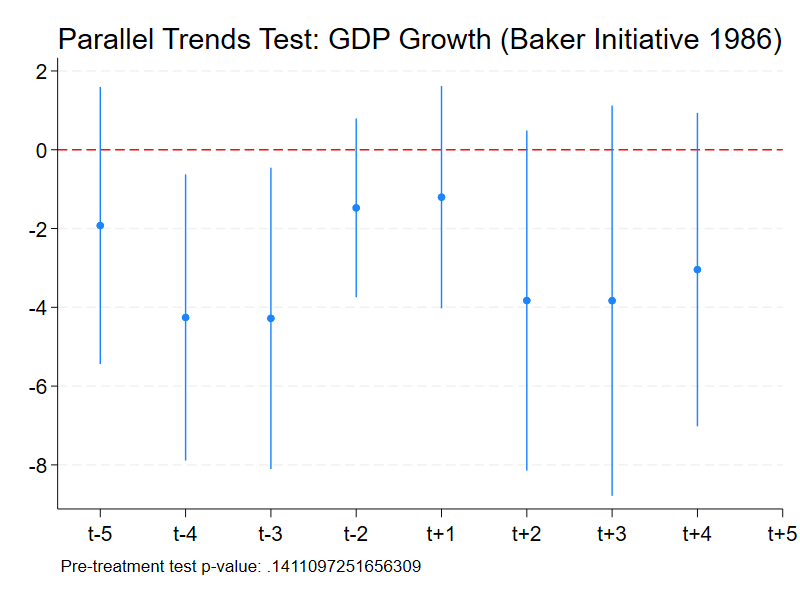
\includegraphics[width=\textwidth]{figures/PT_Baker_GDP.png}
        \caption{Parallel Trend Test 4}
        \label{fig:pt4_eme}
    \end{subfigure}
    \\[1em]
    \begin{subfigure}[b]{0.48\textwidth}
        \centering
        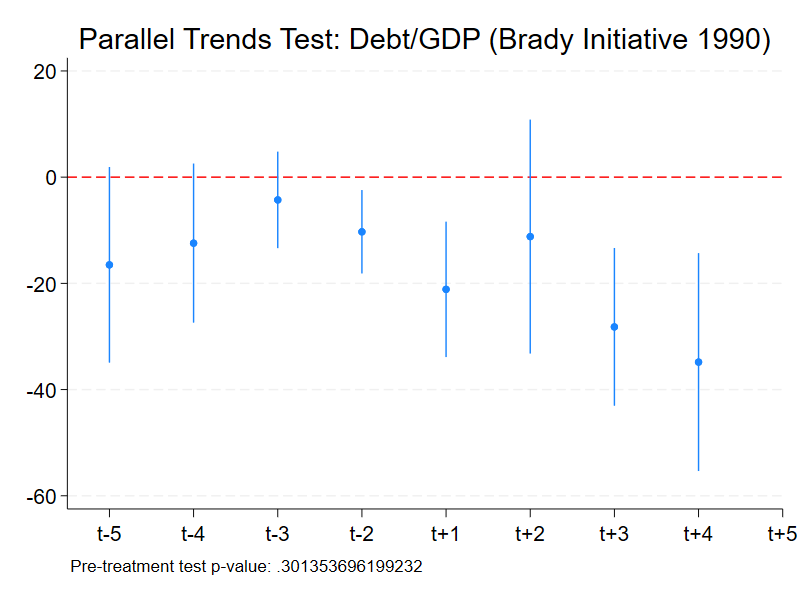
\includegraphics[width=\textwidth]{figures/PT_Brady_Debt.png}
        \caption{Parallel Trend Test 5}
        \label{fig:pt5_eme}
    \end{subfigure}
    \hfill
    \begin{subfigure}[b]{0.48\textwidth}
        \centering
        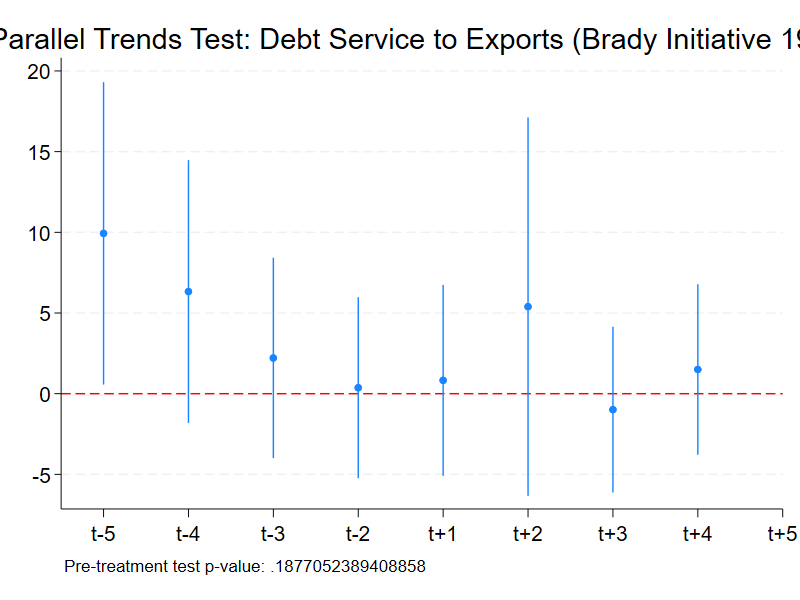
\includegraphics[width=\textwidth]{figures/PT_Brady_DebtServ.png}
        \caption{Parallel Trend Test 6}
        \label{fig:pt6_eme}
    \end{subfigure}
    \\[1em]
    \begin{subfigure}[b]{0.48\textwidth}
        \centering
        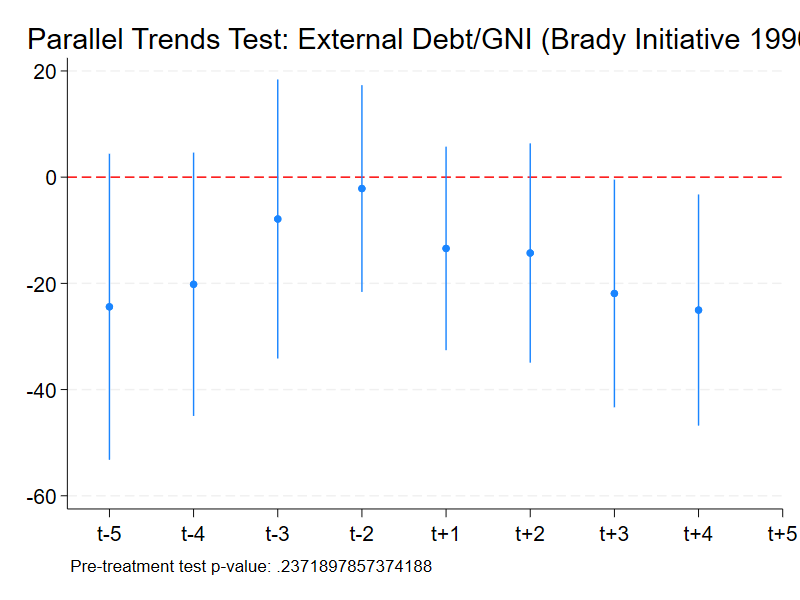
\includegraphics[width=\textwidth]{figures/PT_Brady_ExtDebt.png}
        \caption{Parallel Trend Test 7}
        \label{fig:pt7_eme}
    \end{subfigure}
    \hfill
    \begin{subfigure}[b]{0.48\textwidth}
        \centering
        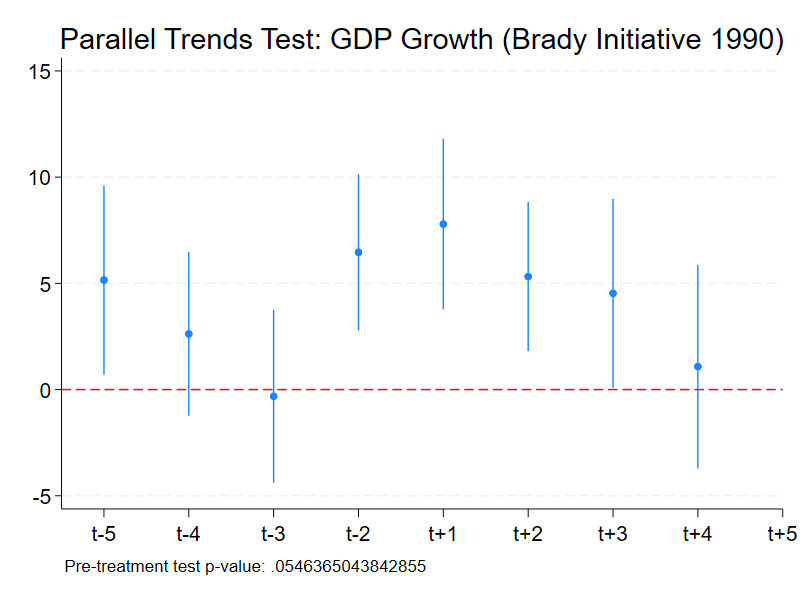
\includegraphics[width=\textwidth]{figures/PT_Brady_GDP.png}
        \caption{Parallel Trend Test 8}
        \label{fig:pt8_eme}
    \end{subfigure}
    \caption{Parallel trend test results for EME case}
    \label{fig:parallel_trends3}
\end{figure}

\begin{figure}[ht!]
    \centering
    \begin{subfigure}[b]{0.48\textwidth}
        \centering
        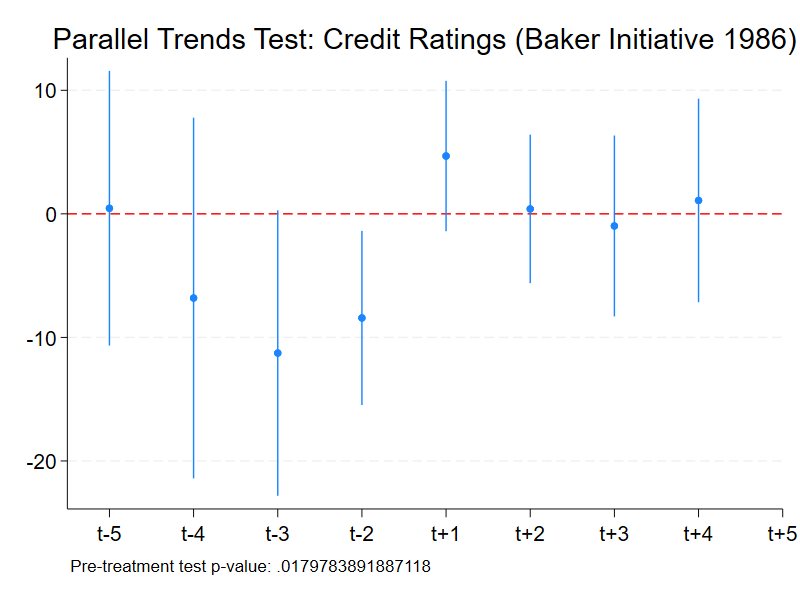
\includegraphics[width=\textwidth]{figures/PT_Baker_Ratings.png}
        \caption{Parallel Trend Test 9}
        \label{fig:pt9_eme}
    \end{subfigure}
    \hfill
    \begin{subfigure}[b]{0.48\textwidth}
        \centering
        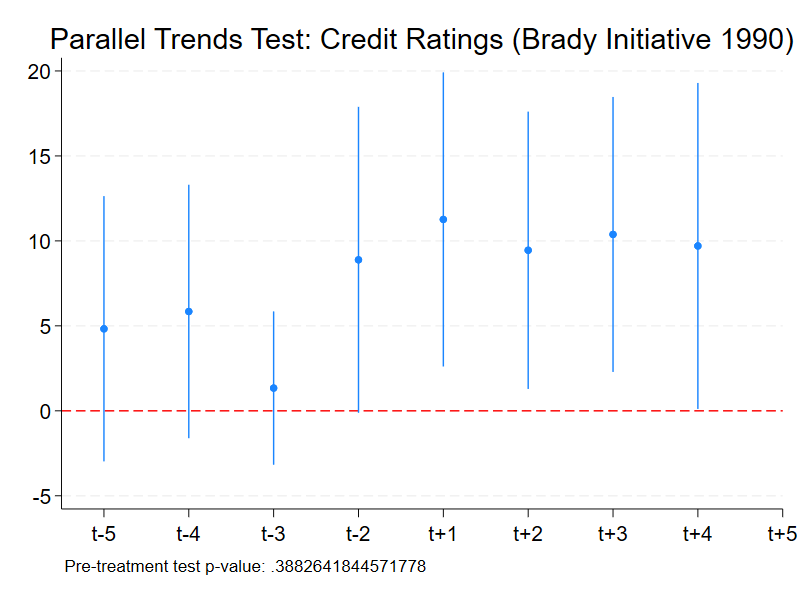
\includegraphics[width=\textwidth]{figures/PT_Brady_Ratings.png}
        \caption{Parallel Trend Test 10}
        \label{fig:pt10_eme}
    \end{subfigure}
    \caption{Parallel trend test results for EME case}
    \label{fig:parallel_trends4}
\end{figure}

In Table 5,
the treatment coefficient for output growth is negative and insignificant for the Baker
episode. Also, debt/GDP continues to grow post-treatment. On the positive side, we
find evidence that the credit ratings of the Baker countries increase significantly more
than the counterfactual (also because the time window includes the 1990/1991 Brady
years). Moreover, the treatment coefficient for debt servicing is negative and marginally
significant, indicating that the Baker plan indeed brought cash flow relief.

\begin{table}[ht!]\centering
\def\sym#1{\ifmmode^{#1}\else\(^{#1}\)\fi}
\caption{Table 5: Baker Initiative (1986) - Difference-in-Difference Analysis}
\renewcommand{\arraystretch}{1.2} % 增加行距
\begin{tabular*}{\textwidth}{@{\hskip\tabcolsep\extracolsep\fill}p{4cm}*{5}{>{\centering\arraybackslash}p{2cm}}}
\hline\hline
            &(1)&(2)&(3)&(4)&(5)\\
            &\parbox{2cm}{\centering Growth, real p.c.}&\parbox{2cm}{\centering Credit Ratings (change)}&\parbox{2cm}{\centering Debt Service to Exports}&\parbox{2cm}{\centering Total Public Debt/GDP}&\parbox{2cm}{\centering External Debt/GNI}\\
\hline
\parbox{4cm}{\raggedright Post-1986 dummy}&  $-1.976$  &  $-5.968^{**}$  &  $-5.758$  &  $-17.214^{**}$  &  $-8.881$  \\
            &  $(1.292)$  &  $(2.328)$ & $(3.426)$   &  $(7.106)$   &  $(6.251)$  \\
[0.5em]
\parbox{4cm}{\raggedright Baker Treatment $\times$ Post-1986}&  $-1.918$&  $6.305^{*}$  &  $-9.049^{*}$&  $22.988^{**}$  &  $17.432$   \\
            &  $(1.329)$   &  $(3.121)$   &  $(4.720)$   &  $(9.360)$   &  $(10.802)$   \\
\hline
Observations&       $275$   &       $279$   &       $189$   &       $226$   &       $199$   \\
R-squared   &       $0.111$   &       $0.200$   &       $0.154$   &       $0.238$   &       $0.189$   \\
Adjusted R² &       $0.077$   &       $0.170$   &       $0.106$   &       $0.203$   &       $0.145$   \\
\hline\hline
\multicolumn{6}{p{0.95\textwidth}}{\footnotesize \textbf{Notes:} This table reports difference-in-difference estimates of the effect of the Baker Initiative on various economic outcomes. Treatment group consists of countries that received Baker Plan debt relief. All regressions include country and year fixed effects. Time window: 1981-1990 (5 years before and after 1986). Standard errors clustered at country level in parentheses. $^*$ p<0.10, $^{**}$ p<0.05, $^{***}$ p<0.01}\\
\end{tabular*}
\end{table}


\begin{table}[ht!]\centering
\def\sym#1{\ifmmode^{#1}\else\(^{#1}\)\fi}
\caption{Table 6: Brady Initiative (1990) - Difference-in-Difference Analysis}
\renewcommand{\arraystretch}{1.2} % 增加行距
\begin{tabular*}{\textwidth}{@{\hskip\tabcolsep\extracolsep\fill}p{4cm}*{5}{>{\centering\arraybackslash}p{2cm}}}
\hline\hline
            &(1)&(2)&(3)&(4)&(5)\\
            &\parbox{2cm}{\centering Growth, real p.c.}&\parbox{2cm}{\centering Credit Ratings (change)}&\parbox{2cm}{\centering Debt Service to Exports}&\parbox{2cm}{\centering Total Public Debt/GDP}&\parbox{2cm}{\centering External Debt/GNI}\\
\hline
\parbox{4cm}{\raggedright Post-1990 dummy}&  $1.207$  &  $5.061^*$  &  $-1.884$  &  $-15.324^{**}$  &  $-10.819$  \\
            &  $(1.350)$  &  $(2.505)$ & $(2.461)$   &  $(7.101)$   &  $(9.069)$  \\
[0.5em]
\parbox{4cm}{\raggedright Brady Treatment $\times$ Post-1990}&  $3.094^{***}$&  $6.991^{**}$  &  $-1.565$&  $-14.514^*$  &  $-1.821$   \\
            &  $(1.046)$   &  $(3.095)$   &  $(3.542)$   &  $(7.377)$   &  $(10.677)$   \\
\hline
Observations&       $270$   &       $270$   &       $190$   &       $233$   &       $200$   \\
R-squared   &       $0.132$   &       $0.242$   &       $0.299$   &       $0.275$   &       $0.089$   \\
Adjusted R² &       $0.099$   &       $0.213$   &       $0.259$   &       $0.242$   &       $0.041$   \\
\hline\hline
\multicolumn{6}{p{0.95\textwidth}}{\footnotesize \textbf{Notes:} This table reports difference-in-difference estimates of the effect of the Brady Initiative on various economic outcomes. Treatment group consists of countries that received Brady Plan debt relief. All regressions include country and year fixed effects. Time window: 1986-1995 (5 years before and after 1990). Standard errors clustered at country level in parentheses. $^*$ p<0.10, $^{**}$ p<0.05, $^{***}$ p<0.01}\\
\end{tabular*}
\end{table}


The most notable change between the Baker and Brady regression results (Tables 5
and 6) is in column (1). The treatment coefficient for real per capita GDP growth turns
positive and highly significant, indicating that the Brady debt relief operation translated
into 3 percentage point higher growth, compared to the counterfactual of non-crisis
emerging markets. This is a sizable coefficient, which resembles that of the 1934
episode (Table 4). Also, the credit ratings of Brady countries see a large improvement
relative to the counterfactual (of 7 IIR index points, on average), while government
debt levels drop significantly more (by 15 percentage points). Surprisingly, however,
we find no significant effect on debt servicing or for total external debt/GDP, possibly
because the actual Brady restructurings took place with a lag in many countries, as
discussed previously.



\section{Staggered DiD Analysis}
According to the author, the Brady Plan was actually implemented in a staggered
fashion, with some countries starting in 1989 and others following until 1995.

To account for this, we use the Callaway-Sant'Anna (2021) staggered difference-in-differences
(CSDID) estimator, which allows for heterogeneous treatment effects and
dynamic treatment effects over time.

\begin{figure}[ht!]
    \centering
    \begin{subfigure}[b]{0.48\textwidth}
        \centering
        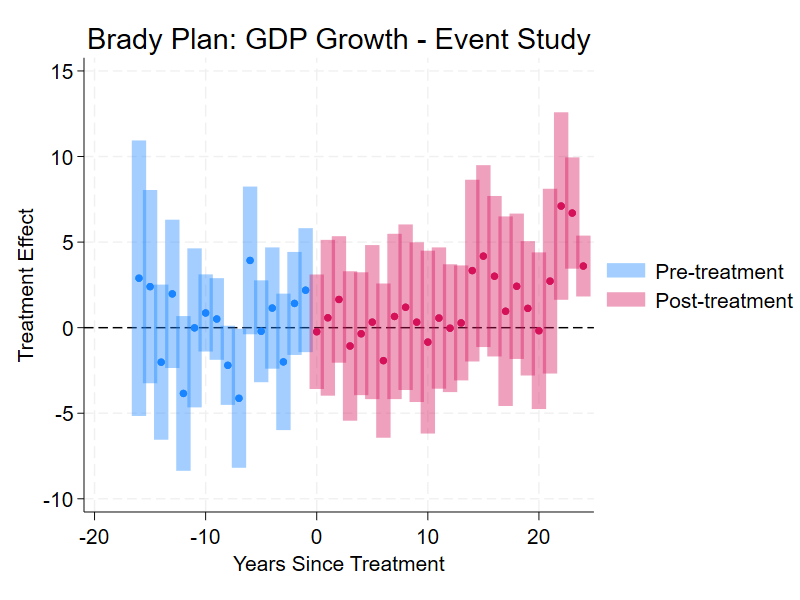
\includegraphics[width=\textwidth]{figures/CS_Brady_Growth_EventStudy.png}
        \caption{Staggered DiD Result 1}
        \label{fig:stag1}
    \end{subfigure}
    \hfill
    \begin{subfigure}[b]{0.48\textwidth}
        \centering
        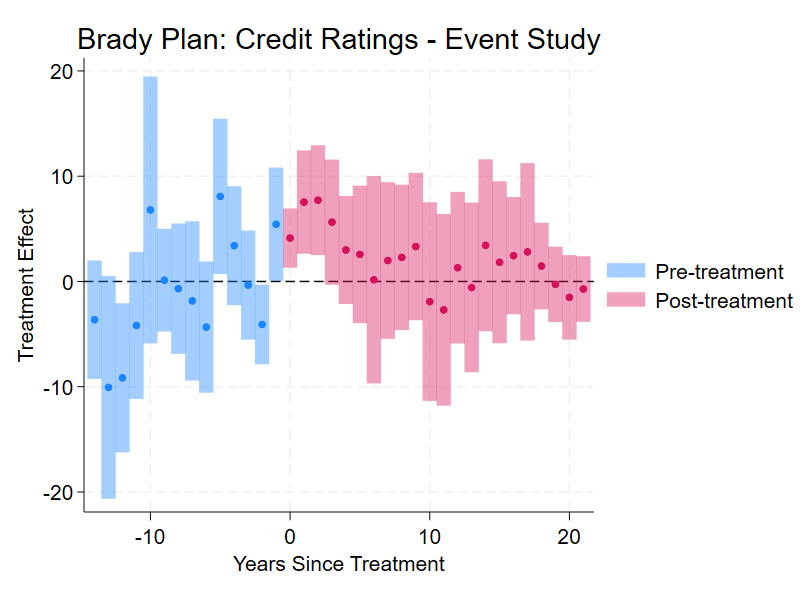
\includegraphics[width=\textwidth]{figures/CS_Brady_Ratings_EventStudy.png}
        \caption{Staggered DiD Result 2}
        \label{fig:stag2}
    \end{subfigure}
    \\[1em]
    \begin{subfigure}[b]{0.48\textwidth}
        \centering
        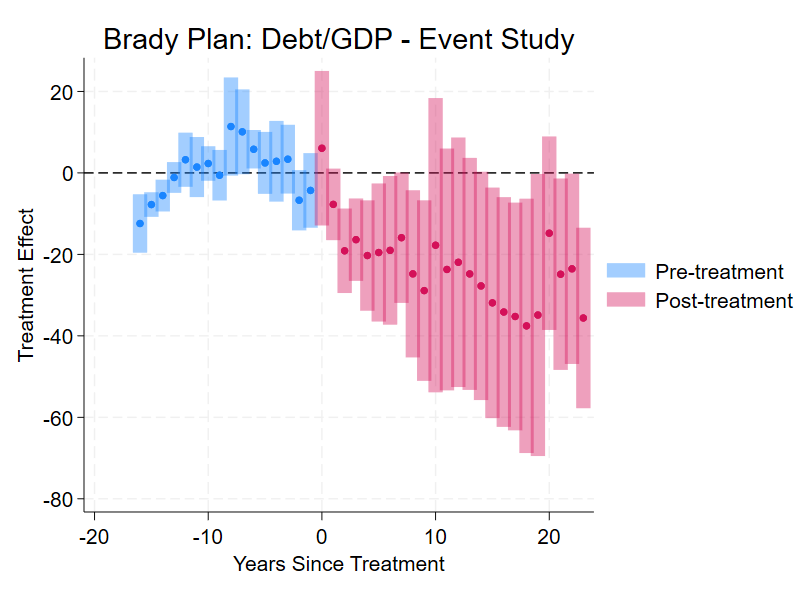
\includegraphics[width=\textwidth]{figures/CS_Brady_Debt_EventStudy.png}
        \caption{Staggered DiD Result 3}
        \label{fig:stag3}
    \end{subfigure}
    \hfill
    \begin{subfigure}[b]{0.48\textwidth}
        \centering
        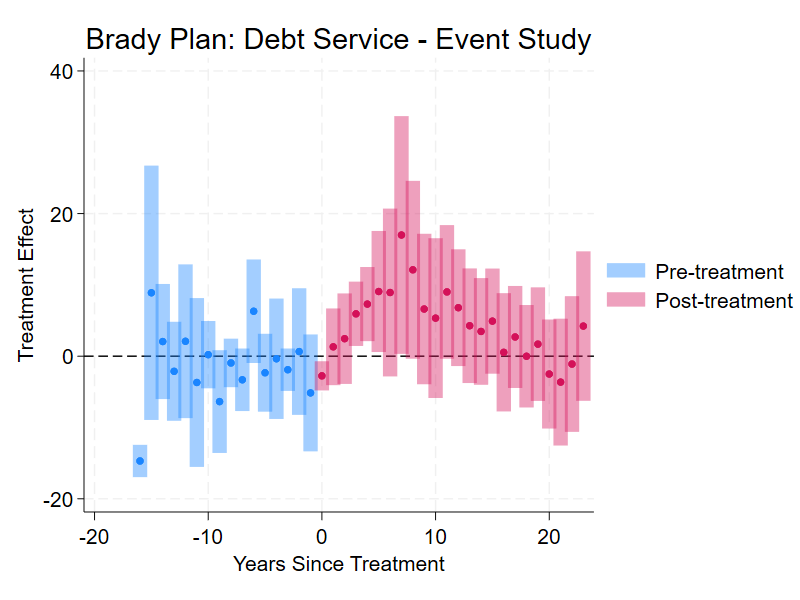
\includegraphics[width=\textwidth]{figures/CS_Brady_DebtService_EventStudy.png}
        \caption{Staggered DiD Result 4}
        \label{fig:stag4}
    \end{subfigure}
    \\[1em]
    \begin{subfigure}[b]{0.48\textwidth}
        \centering
        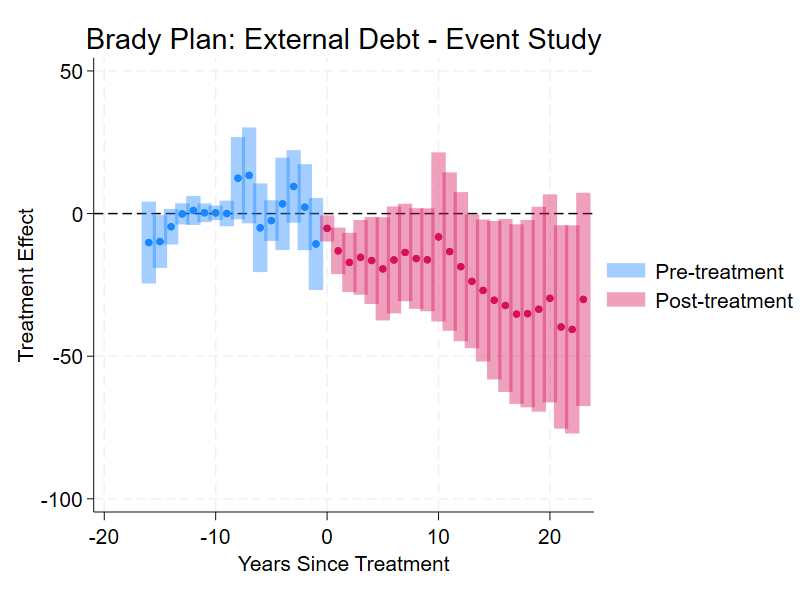
\includegraphics[width=\textwidth]{figures/CS_Brady_ExtDebt_EventStudy.png}
        \caption{Staggered DiD Result 5}
        \label{fig:stag5}
    \end{subfigure}
    \caption{Staggered Difference-in-Differences Analysis Results}
    \label{fig:staggered_did}
\end{figure}

To see it in a more clear way, we also write the results into a table:

\begin{table}[ht!]\centering
\def\sym#1{\ifmmode^{#1}\else\(^{#1}\)\fi}
\caption{Brady Plan (1989-1995) - Callaway-Sant'Anna Staggered Difference-in-Differences Analysis}
\renewcommand{\arraystretch}{1.2} % 增加行距
\begin{tabular*}{\textwidth}{@{\hskip\tabcolsep\extracolsep\fill}p{4cm}*{5}{>{\centering\arraybackslash}p{2cm}}}
\hline\hline
            &(1)&(2)&(3)&(4)&(5)\\
            &\parbox{2cm}{\centering Growth, real p.c.}&\parbox{2cm}{\centering Credit Ratings (change)}&\parbox{2cm}{\centering Debt Service to Exports}&\parbox{2cm}{\centering Total Public Debt/GDP}&\parbox{2cm}{\centering External Debt/GNI}\\
\hline
\parbox{4cm}{\raggedright Average Treatment Effect on Treated (ATT)}&  $1.005$  &  $2.331$  &  $5.047$  &  $-22.587^{**}$  &  $-20.799^{**}$  \\
            &  $(1.923)$  &  $(2.494)$ & $(3.299)$   &  $(9.722)$   &  $(9.550)$  \\
[0.5em]
\hline
Treatment Countries&       $16$   &       $16$   &       $16$   &       $16$   &       $16$   \\
Control Countries   &       $24$   &       $24$   &       $24$   &       $24$   &       $24$   \\
% Treatment Period     &       \multicolumn{5}{c}{$1989-1995$}   \\
% Method              &       \multicolumn{5}{c}{Callaway-Sant'Anna (2021)}   \\
\hline\hline
\multicolumn{6}{p{0.95\textwidth}}{\footnotesize \textbf{Notes:} This table presents average treatment effects on the treated (ATT) from the Callaway and Sant'Anna (2021) staggered difference-in-differences estimator using actual Brady Plan implementation dates by country. Treatment timing varies from 1989-1995: Mexico, Philippines, Costa Rica (1989); Uruguay, Venezuela (1990); Nigeria (1991); Argentina, Brazil (1992); Bolivia, Bulgaria, Dominican Republic, Jordan (1993); Ecuador, Poland (1994); Panama, Peru (1995). Control group consists of emerging market economies that never implemented Brady agreements. The method accounts for treatment effect heterogeneity across cohorts and time periods using doubly robust inverse probability weighting (DRIPW). Standard errors clustered at country level in parentheses. $^*$ p<0.10, $^{**}$ p<0.05, $^{***}$ p<0.01}\\
\end{tabular*}
\end{table}


\begin{enumerate}[label=(\arabic*),leftmargin=1.25cm]
    \item \textbf{Real per-capita GDP growth}.  
    The point estimate of \(\text{ATT}=1.005\) (s.e.\;1.923) is economically small and statistically insignificant.\footnote{All hypothesis tests use two-sided $t$-statistics with 39 degrees of freedom.}  
    Hence, short-run output gains attributable solely to the Brady restructuring appear limited.

    \item \textbf{Credit-rating upgrades}.  
    The estimated improvement of \(2.331\) notches (s.e.\;2.494) is likewise imprecisely measured, suggesting that sovereign creditworthiness did not accelerate immediately after restructuring.

    \item \textbf{Debt-service pressure}.  
    The debt-service-to-exports ratio rises by \(5.047\) percentage points (s.e.\;3.299) but remains insignificant.  
    A mechanical uptick is plausible because coupon payments on the new Brady bonds were front-loaded, even though principal obligations were reduced.

    \item \textbf{Public-debt burden}.  
    A statistically significant fall of \(-22.587^{**}\) percentage points of GDP (s.e.\;9.722) confirms that the Brady exchanges achieved their primary aim: \emph{a sizable reduction in public debt stocks}.

    \item \textbf{External indebtedness}.  
    External debt drops by \(-20.799^{**}\) percentage points of GNI (s.e.\;9.550).  
    The comparable magnitude across the two debt ratios underscores that the relief was broad-based, not merely an accounting reshuffle between domestic and foreign holders.
\end{enumerate}

\paragraph{Methodological strengths.}
The staggered estimator weights cohort-specific counterfactuals, eliminating negative-weight bias inherent in traditional two-way fixed effects when treatment timing is staggered.  
Doubly robust inverse-probability weighting (DRIPW) further guards against misspecification in both the propensity-score and outcome equations, enhancing credibility.

\paragraph{Economic implications.}
\begin{itemize}[leftmargin=0.9cm]
    \item \emph{Debt relief first, growth later.}  The significant contraction in debt ratios signals successful balance-sheet repair.  However, growth dividends are not immediate; structural reforms and a longer horizon may be required for debt relief to translate into higher output.
    \item \emph{Market sentiment lags policy action.}  Credit-rating agencies reacted cautiously, consistent with historical evidence that ratings improve only after sustained fiscal consolidation.
    \item \emph{Policy design.}  Future restructurings should pair liability management with complementary reforms (e.g.\ trade liberalisation, financial-sector deepening) to accelerate real-sector recovery.
\end{itemize}

\paragraph{Limitations.}
The evaluation window (1989-1995) captures only the first six years after each country's exchange.  If growth effects materialise with longer lags, the present estimates are lower bounds.  Moreover, macro-shocks in the early 1990s (e.g.\ the Tequila crisis) may attenuate observed treatment effects despite the DiD controls.
 
%\chapter{Code replication}
\label{chapter:codemodel}

\section{War Period}

\subsection{Define War Samples \& Counterfactuals}
\begin{itemize}
    \item Defaulters: 18 countries, Austria, Belgium, Czechoslovakia, Estonia, France, Greece, Yugoslavia, Hungary, Italy, Latvia, Lithuania, Poland, Romania, UK, Germany, Australia, Portugal, New Zealand.
    \item No credit event: Finland, Norway, Sweden, Switzerland, Denmark, Ireland, Spain
	\item Extension: Russia, Japan, China, Bulgaria, Turkey, Thailand; Argentina, Uruguay, Chile, Brazil, Colombia, Mexico, Peru, Venezuela
\end{itemize}

Final data samples are set as below:
\begin{itemize}
    \item WarSmallSample: defaulters and no defaulters from Europe;
    \item WarLatAmSample: defaulters and no defaulters from Europe and Latin America;
    \item WarNonLatAmSample: defaulters and no defaulters from Europe and non-Latin America;
    \item WarAllSample: defaulters and no defaulters from all countries.
    \item WarCounterfactual: no defaulters from Europe, Latin America and Non Latin America.
\end{itemize}


\subsection{Time Windows}
1931 Hoover Moratorium and 1934 Default as the baseline $T$, $T-5, T+5$ as the time window.
Normalize Debt index and GDP index with respect to both baselines.
\begin{itemize}
    \item Debt index: -5 to 5;
    \item FDP index: real GDP divided by baseline real GDP;
    \item Rating index: moody's rating divided by baseline moody's rating, in numerical form, from 1 to 9, by checking the data of Switzerland, we believe 9 represents AAA.
\end{itemize}

\begin{figure}[ht!]
    \centering
    \begin{subfigure}[b]{0.48\textwidth}
        \centering
        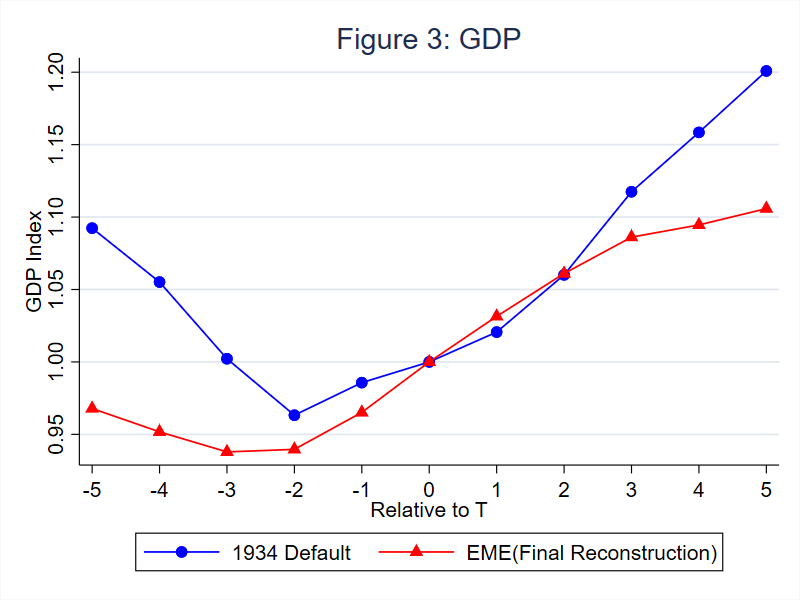
\includegraphics[width=\textwidth]{figures/Figure3_GDP_Comparison.png}
        \caption{Real per capita GDP around debt relief events (exit from default) in middle- to high-
income emerging markets (1978-2010) and advanced economies (1934).}
        \label{fig:3}
    \end{subfigure}
    \hfill
    \begin{subfigure}[b]{0.48\textwidth}
        \centering
        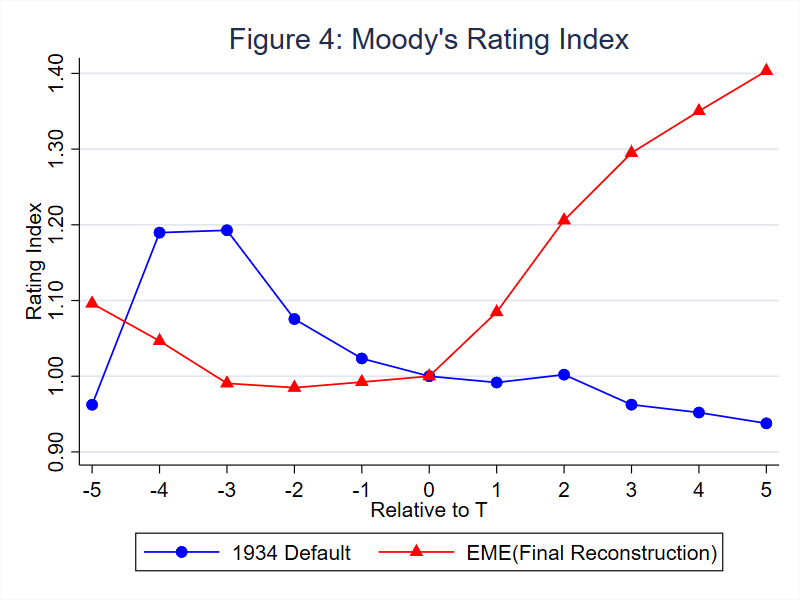
\includegraphics[width=\textwidth]{figures/Figure4_Rating_Comparison.png}
        \caption{Total external debt to GDP (in \%) around debt relief events (exit from default) in
        middle- to high-income emerging markets (1978-2010) and advanced economies (1934).}
        \label{fig:4}
    \end{subfigure}
\end{figure}

\begin{figure}[ht!]
    \centering
    \begin{subfigure}[b]{0.48\textwidth}
        \centering
        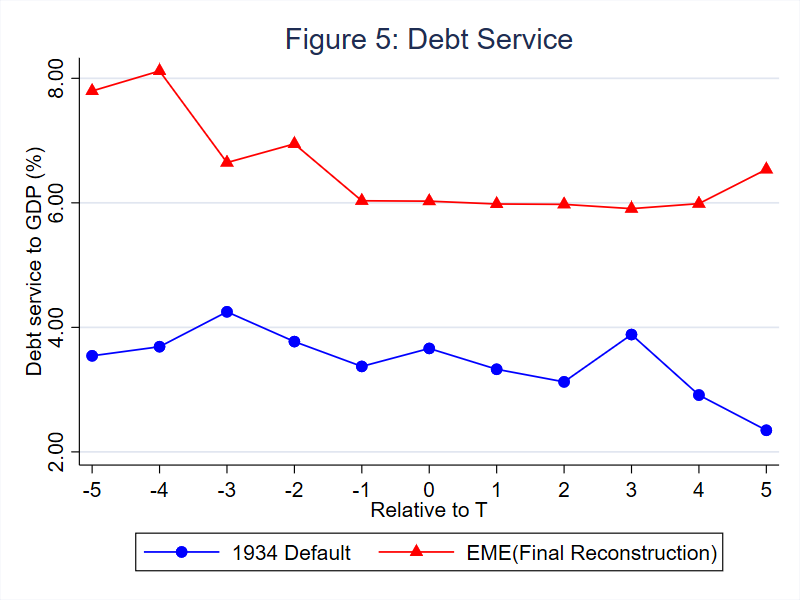
\includegraphics[width=\textwidth]{figures/Figure5_DebtService_Comparison.png}
        \caption{Total debt service to GDP (in \%) around debt relief events (exit from default) in
        middle- to high-income emerging markets (1978-2010) and advanced economies (1934).}
        \label{fig:5}
    \end{subfigure}
    \hfill
    \begin{subfigure}[b]{0.48\textwidth}
        \centering
        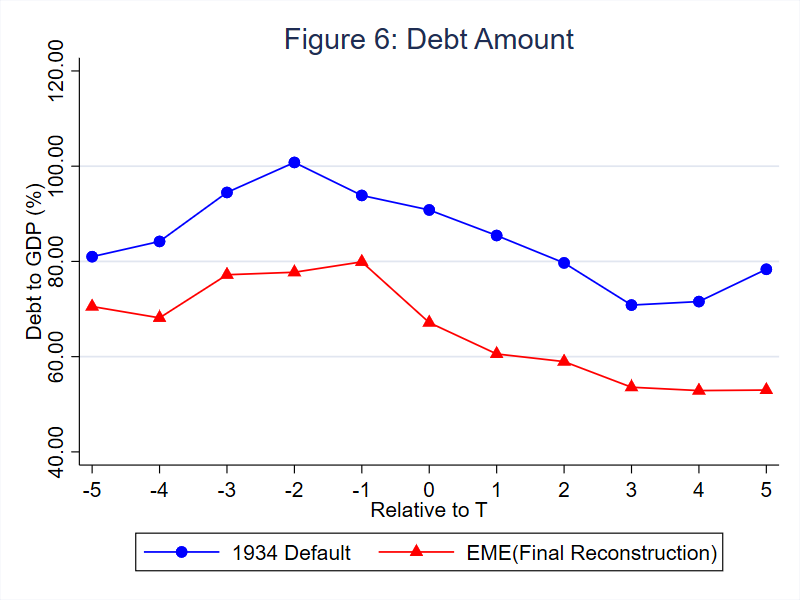
\includegraphics[width=\textwidth]{figures/Figure6_DebtStock_Comparison.png}
        \caption{Debt to GDP (in \%) around debt relief events (exit from default) in middle- to high-
income emerging markets (1978-2010) and advanced economies (1934).}
        \label{fig:6}
    \end{subfigure}
\end{figure}

\subsection{Parallel trend test}
We found out that the author only used the data to make descriptive analysis, but did not
use the data to make a parallel trend test. So, we work on the parallel trend test ourselves, and the results are as below.

To see the results more easily, we write into a matrix:
\begin{table}[ht!]
\centering
\begin{tabular}{lccc}
\toprule
Variable & P‐Value & Pass (5\%) & Pass (10\%) \\
\midrule
GDP\_Growth\_1934\_l   & 0.52529567 & 1 & 1 \\
GDP\_Growth\_1934\_e   & 0.94559858 & 1 & 1 \\
Ratings\_1934          & 0.04996219 & 0 & 0 \\
DebtServ\_1934\_l      & 0.13978740 & 1 & 1 \\
DebtServ\_1934\_e      & 0.51155188 & 1 & 1 \\
Debt\_GDP\_1934\_l     & 0.12776463 & 1 & 1 \\
Debt\_GDP\_1934\_e     & 0.25006164 & 1 & 1 \\
ExtDebt\_1934          & 0.06999843 & 1 & 0 \\
\midrule
GDP\_Growth\_1931\_l   & 0.57373095 & 1 & 1 \\
GDP\_Growth\_1931\_e   & 0.23592213 & 1 & 1 \\
Ratings\_1931          & 0.41062027 & 1 & 1 \\
DebtServ\_1931\_l      & 0.28772333 & 1 & 1 \\
DebtServ\_1931\_e      & 0.39504800 & 1 & 1 \\
Debt\_GDP\_1931\_l     & 0.01403155 & 0 & 0 \\
Debt\_GDP\_1931\_e     & 0.07416818 & 1 & 0 \\
ExtDebt\_1931          & 0.01362215 & 0 & 0 \\
\bottomrule
\end{tabular}
\caption{P-values and pass/fail indicators at 5\% and 10\% levels}
\label{tab:pass_tests}
\end{table}


From this table, we could see that main results are available, most variables pass the test,
only two variables failed, which we need to interpret with caution:
\begin{itemize}
    \item Credit rating results for 1934
    \item Debt/GDP ratio and external debt/GDP ratio results for 1931
\end{itemize}

\begin{figure}[ht!]
    \centering
    \begin{subfigure}[b]{0.48\textwidth}
        \centering
        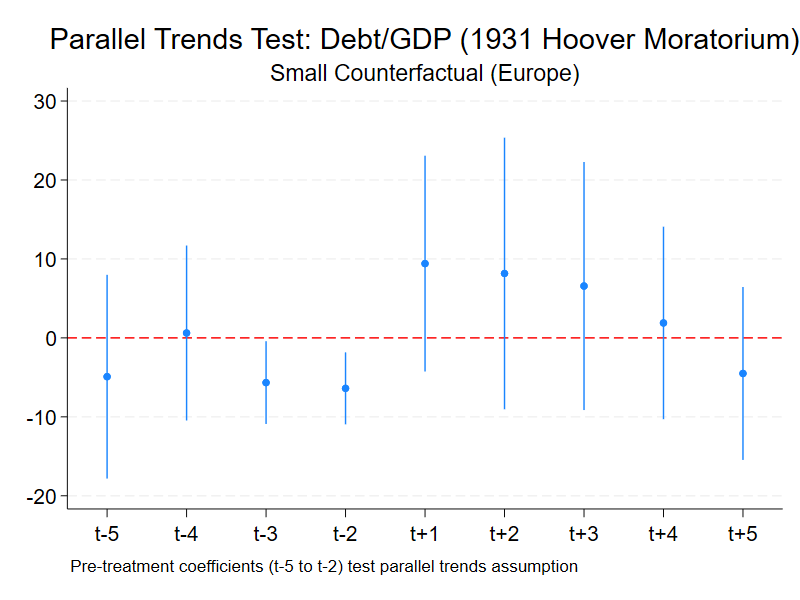
\includegraphics[width=\textwidth]{figures/PT_Debt_1931_Small.png}
        \caption{Parallel Trend Test 1}
        \label{fig:pt1}
    \end{subfigure}
    \hfill
    \begin{subfigure}[b]{0.48\textwidth}
        \centering
        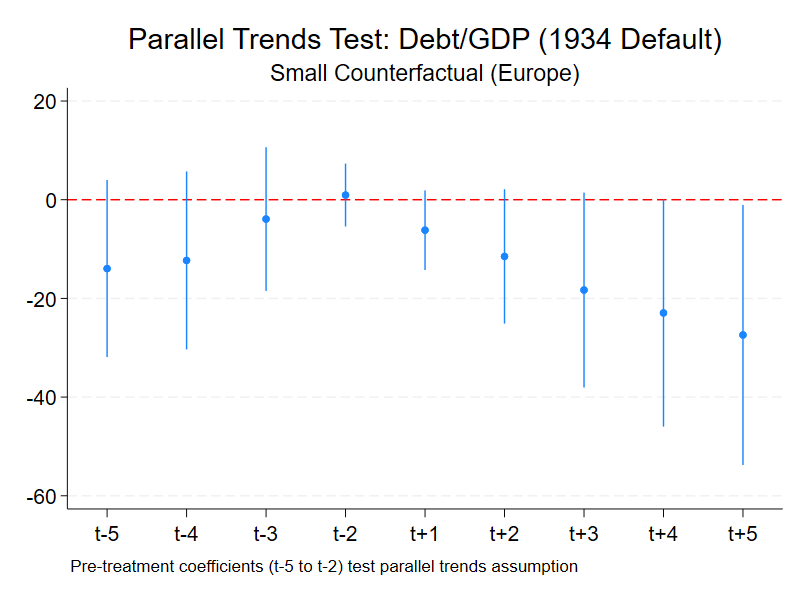
\includegraphics[width=\textwidth]{figures/PT_Debt_1934_Small.png}
        \caption{Parallel Trend Test 2}
        \label{fig:pt2}
    \end{subfigure}
    \\[1em]
    \begin{subfigure}[b]{0.48\textwidth}
        \centering
        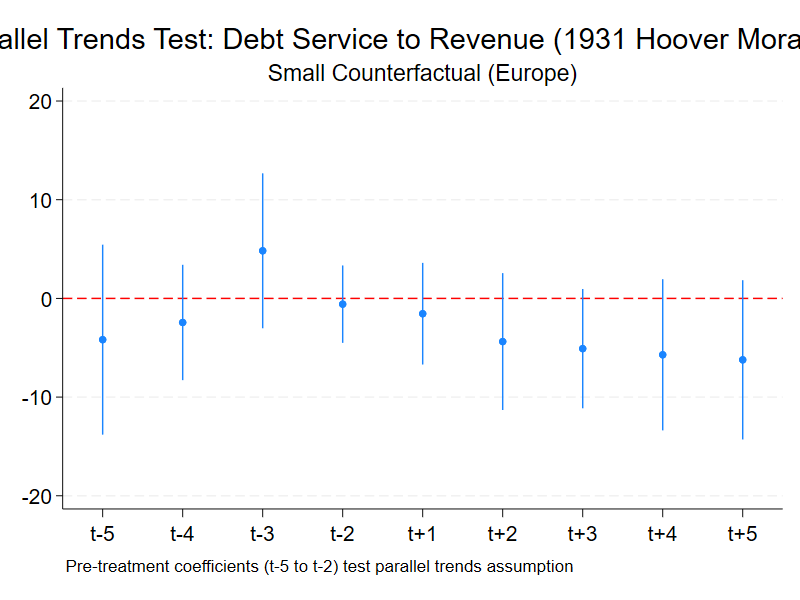
\includegraphics[width=\textwidth]{figures/PT_DebtServ_1931_Small.png}
        \caption{Parallel Trend Test 3}
        \label{fig:pt3}
    \end{subfigure}
    \hfill
    \begin{subfigure}[b]{0.48\textwidth}
        \centering
        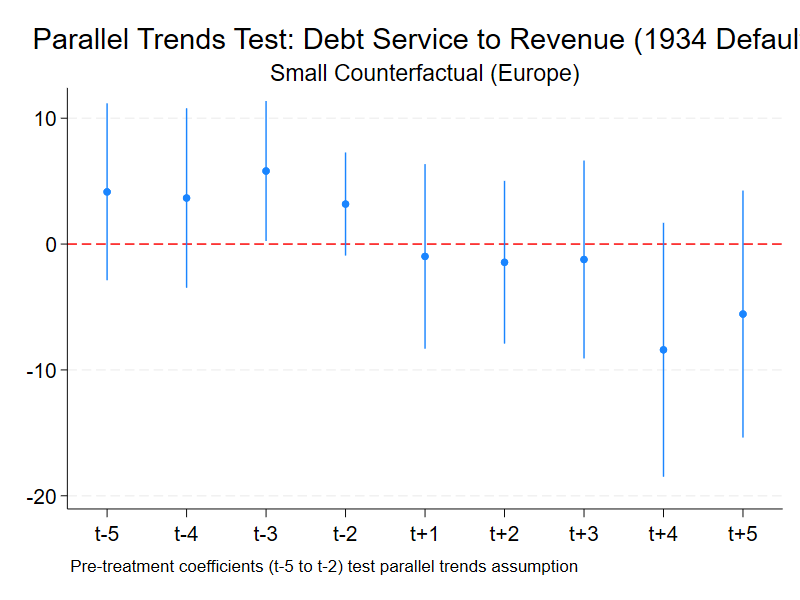
\includegraphics[width=\textwidth]{figures/PT_DebtServ_1934_Small.png}
        \caption{Parallel Trend Test 4}
        \label{fig:pt4}
    \end{subfigure}
    \\[1em]
    \begin{subfigure}[b]{0.48\textwidth}
        \centering
        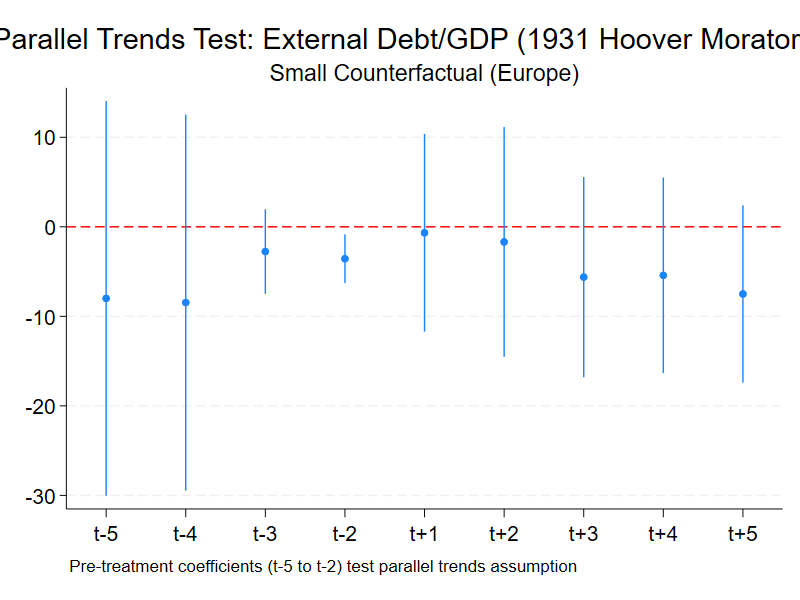
\includegraphics[width=\textwidth]{figures/PT_ExtDebt_1931.png}
        \caption{Parallel Trend Test 5}
        \label{fig:pt5}
    \end{subfigure}
    \hfill
    \begin{subfigure}[b]{0.48\textwidth}
        \centering
        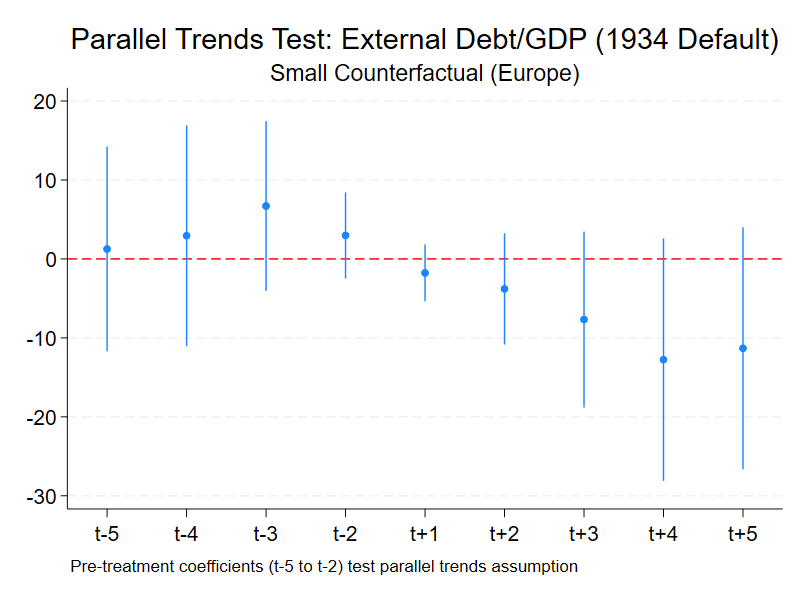
\includegraphics[width=\textwidth]{figures/PT_ExtDebt_1934.png}
        \caption{Parallel Trend Test 6}
        \label{fig:pt6}
    \end{subfigure}
    \\[1em]
    \begin{subfigure}[b]{0.48\textwidth}
        \centering
        \includegraphics[width=\textwidth]{figures/PT_GDP_1931_Large.png}
        \caption{Parallel Trend Test 7}
        \label{fig:pt7}
    \end{subfigure}
    \hfill
    \begin{subfigure}[b]{0.48\textwidth}
        \centering
        \includegraphics[width=\textwidth]{figures/PT_GDP_1931_Small.png}
        \caption{Parallel Trend Test 8}
        \label{fig:pt8}
    \end{subfigure}
    \caption{Parallel trend test results for different country samples and variables}
    \label{fig:parallel_trends}
\end{figure}

\begin{figure}[ht!]
    \centering
    \begin{subfigure}[b]{0.48\textwidth}
        \centering
        \includegraphics[width=\textwidth]{figures/PT_GDP_1934_Large.png}
        \caption{Parallel Trend Test 9}
        \label{fig:pt9}
    \end{subfigure}
    \hfill
    \begin{subfigure}[b]{0.48\textwidth}
        \centering
        \includegraphics[width=\textwidth]{figures/PT_GDP_1934_Small.png}
        \caption{Parallel Trend Test 10}
        \label{fig:pt10}
    \end{subfigure}
    \hfill
    \begin{subfigure}[b]{0.48\textwidth}
        \centering
        \includegraphics[width=\textwidth]{figures/PT_Ratings_1931.png}
        \caption{Parallel Trend Test 11}
        \label{fig:pt11}
    \end{subfigure}
    \hfill
    \begin{subfigure}[b]{0.48\textwidth}
        \centering
        \includegraphics[width=\textwidth]{figures/PT_Ratings_1934.png}
        \caption{Parallel Trend Test 12}
        \label{fig:pt12}
    \end{subfigure}
    \caption{Parallel trend test results for different country samples and variables}
    \label{fig:parallel_trends2}
\end{figure}

\subsection{DID Analysis}

The Brady target group includes all middle-income
EMs with a Brady deal, namely Argentina, Brazil, Bulgaria, Costa Rica, Dominican
Republic, Ecuador, Jordan, Mexico, Panama, Peru, Poland, Uruguay, and Venezuela.
The Baker country sample is the same, plus Chile, which was a target country in the
mid-1980s, but were not part of the “Brady bunch”.

The baseline counterfactual includes all middle- and high-income countries(regions)
that did not default nor received debt relief in this period and for which we have data,
namely China, Colombia, Czech Republic, Egypt, Hungary, India, Israel, Malaysia,
Mauritius, Singapore, South Korea, Taiwan, Thailand, and Turkey.

We start with the Hoover Moratorium of 1931 and take a preliminary view of the
data.

\begin{figure}[ht!]
    \centering
    \includegraphics[width=0.95\textwidth]{figures/Figure8_GDP_trends_1931_1934.png}
    \caption{GDP trends around 1931 and 1934}
    \label{fig:8}
\end{figure}

\begin{figure}[ht!]
    \centering
    \begin{subfigure}[b]{0.48\textwidth}
        \centering
        \includegraphics[width=\textwidth]{figures/figc5_a.png}
        \caption{Residual GDP Growth}
        \label{fig:c5a}
    \end{subfigure}
    \hfill
    \begin{subfigure}[b]{0.48\textwidth}
        \centering
        \includegraphics[width=\textwidth]{figures/figc5_b.png}
        \caption{Credit Ratings}
        \label{fig:c5b}
    \end{subfigure}
    \\[1em]
    \begin{subfigure}[b]{0.48\textwidth}
        \centering
        \includegraphics[width=\textwidth]{figures/figc5_c.png}
        \caption{Debt Service to Revenue}
        \label{fig:c5c}
    \end{subfigure}
    \hfill
    \begin{subfigure}[b]{0.48\textwidth}
        \centering
        \includegraphics[width=\textwidth]{figures/figc5_d.png}
        \caption{Debt to GDP}
        \label{fig:c5d}
    \end{subfigure}
    \caption{Economic indicators comparison between treatment and control groups}
    \label{fig:c5}
\end{figure}

The figures compare the development of our main economic indicators for treatment and control groups,
where the control groups is our baseline sample of European non-defaulters.
Figure 8 (left panel) shows that the growth performance of the treatment group is significantly worse
than that of the counterfactual around 1931. 

Panel B: country
heterogeneity by showing residuals from a regression of annual real p.c. growth on a
constant and country-specific dummies. Residual growth declines markedly for both
groups prior to 1931 and recovers strongly afterwards, but there is no evidence that
treatment countries perform better than the counterfactual.

Panel C: The picture is similarly
bleak with regard to Moody's credit ratings, which decline across the board after 1931,
with no notable difference between the two groups. 

Panel D: Similarly, the debt/GDP
level does not decline significantly more for the target countries. Only the
debt servicing burden improves, as payments to revenue drop relatively more than
those countries not receiving relief.

\subsection{Results of DID}
The results are more notable for the 1934 debt relief spell. Table 4 indicates that
real per capita growth is 4.7 percentage points higher for treated countries in the post-
1934 period, with a highly significant coefficient (column (1)). Moreover, the debt
levels decrease significantly (columns (6) and (8)), compared to the counterfactual on
European non-defaulters. We find no significant coefficient for debt servicing (column
(4)) and a highly significant negative coefficient for ratings. These results, however,
are rather sensitive to the choice of counterfactual, as can be seen in columns (2),
(5), and (7), which use the “World” counterfactual including European, Asian, and
South American countries. The treatment coefficient for debt servicing becomes highly
significant and large, while the coefficient for debt/GDP turns insignificant. Notably,
however, the growth coefficient remains large and significant across all counterfactuals
chosen, albeit sometimes only at the 10\% level.

\begin{sidewaystable}[ht!]\centering
\def\sym#1{\ifmmode^{#1}\else\(^{#1}\)\fi}
\caption{Table 3: 1931 Hoover Moratorium - Difference-in-Difference Analysis}
\renewcommand{\arraystretch}{1.2} % 增加行距
\begin{tabular*}{\textwidth}{@{\hskip\tabcolsep\extracolsep\fill}p{3.75cm}*{8}{>{\centering\arraybackslash}p{2.25cm}}}
\hline\hline
            &(1)&(2)&(3)&(4)&(5)&(6)&(7)&(8)\\
            &\parbox{2.25cm}{\centering Growth, real p.c.\\Small (Europe)}&\parbox{2.25cm}{\centering Growth, real p.c.\\Large (World)}&\parbox{2.25cm}{\centering Credit Ratings (change)\\Small (Europe)}&\parbox{2.25cm}{\centering Debt Service to Revenue\\Small (Europe)}&\parbox{2.25cm}{\centering Debt Service to Revenue\\Large (World)}&\parbox{2.25cm}{\centering Total Public Debt/GDP\\Small (Europe)}&\parbox{2.25cm}{\centering Total Public Debt/GDP\\Large (World)}&\parbox{2.25cm}{\centering External Debt/GDP\\Small (Europe)}\\
\hline
\parbox{3cm}{\raggedright Post-intervention dummy (after 1931)}&  $4.922^{**}$  &  $8.329^{***}$  &  $3.752$  &  $-1.064$  &  $-3.882^{**}$&  $-10.011^{*}$  &  $-7.900^{*}$ &  $-9.086^{**}$  \\
            &  $(2.335)$  &  $(1.724)$ & $(3.377)$   &  $(1.880)$   &  $(1.854)$  &  $(4.854)$  &  $(4.240)$  & $(3.687)$   \\
[0.5em]
\parbox{3cm}{\raggedright Treatment (war debt moratorium) $\times$ post-intervention dummy}&  $2.598^{*}$&  $0.862$  &  $-5.655$&  $-4.310^{*}$  &  $-3.390$   &  $7.312$ &  $3.822$   &  $-0.508$ \\
            &  $(1.360)$   &  $(1.333)$   &  $(4.202)$   &  $(2.392)$   &  $(2.335)$   &  $(6.936)$   &  $(6.899)$   &  $(5.610)$   \\
[0.5em]
Constant    &  $-4.072^{***}$&  $-4.489^{***}$&  $0.906$   &  $24.360^{***}$&  $23.973^{***}$&  $69.849^{***}$&  $61.471^{***}$&  $32.183^{***}$\\
            &  $(0.839)$   &  $(1.160)$   &  $(2.058)$   &  $(1.215)$   &  $(0.990)$   &  $(1.872)$   &  $(1.695)$   &  $(2.174)$   \\
\hline
Observations&         237   &         373   &         230   &         223   &         326   &         172   &         248   &         167   \\
Adjusted R² &       0.237   &       0.206   &       0.185   &       0.043   &       0.062   &       0.166   &       0.199   &       0.007   \\
\hline\hline
\multicolumn{9}{p{0.95\textwidth}}{\footnotesize \textbf{Notes:} This table reports difference-in-difference estimates of the effect of the 1931 Hoover Moratorium on various economic outcomes. Treatment group consists of 18 countries that received war debt relief. Small counterfactual includes European non-defaulters; Large counterfactual adds Latin American and other countries. All regressions include country and year fixed effects. Standard errors clustered at country level in parentheses. $^*$ p<0.10, $^{**}$ p<0.05, $^{***}$ p<0.01}\\
\end{tabular*}
\end{sidewaystable}


When we are working on Table3, we found out a bug:
the data of column (3), (4), (5) might be in the wrong order, the correct order of data should be (5), (3), (4).

Also, the post-intervention dummy (after 1931) is very different from authors' result, we also tried to drop the year fixed effect, but the result is still different.
(We tried to run authors' original code, and the results are the same as what we get, not what's in the table of this paper.)

According to the authors based on their result, `The only $\beta_2$ coefficients that are marginally significant are those of GDP and of credit ratings',
but as we could see from our table, only credit ratings and debt service to revenue in treated countries are insignificant.

\begin{figure}[ht!]
    \centering
    \includegraphics[width=0.95\textwidth]{figures/table3_original.png}
    \caption{Table 3 Original}
    \label{fig:table3_original}
\end{figure}

\begin{figure}[ht!]
    \centering
    \includegraphics[width=0.95\textwidth]{figures/col3_tab3_stata.png}
    \caption{Table 3 Col 3}
    \label{fig:table3_col3}
\end{figure}

\begin{figure}[ht!]
    \centering
    \includegraphics[width=0.95\textwidth]{figures/col4_tab3_stata.png}
    \caption{Table 3 Col 4}
    \label{fig:table3_col4}
\end{figure}

\begin{sidewaystable}[ht!]\centering
\def\sym#1{\ifmmode^{#1}\else\(^{#1}\)\fi}
\caption{Table 4: 1934 Summer Defaults - Difference-in-Difference Analysis}
\renewcommand{\arraystretch}{1.2} % 增加行距
\begin{tabular*}{\textwidth}{@{\hskip\tabcolsep\extracolsep\fill}p{3.75cm}*{8}{>{\centering\arraybackslash}p{2.25cm}}}
\hline\hline
            &(1)&(2)&(3)&(4)&(5)&(6)&(7)&(8)\\
            &\parbox{2.25cm}{\centering Growth, real p.c.\\Small (Europe)}&\parbox{2.25cm}{\centering Growth, real p.c.\\Large (World)}&\parbox{2.25cm}{\centering Credit Ratings (change)\\Small (Europe)}&\parbox{2.25cm}{\centering Debt Service to Revenue\\Small (Europe)}&\parbox{2.25cm}{\centering Debt Service to Revenue\\Large (World)}&\parbox{2.25cm}{\centering Total Public Debt/GDP\\Small (Europe)}&\parbox{2.25cm}{\centering Total Public Debt/GDP\\Large (World)}&\parbox{2.25cm}{\centering External Debt/GDP\\Small (Europe)}\\
\hline
\parbox{3cm}{\raggedright Post-intervention dummy (after 1934)}&  $-1.905$  &  $-0.772$  &  $4.527^*$  &  $-4.284$  &  $-5.094^{***}$&  $-9.030$  &  $-9.602^{**}$ &  $-3.487$  \\
            &  $(1.320)$  &  $(1.398)$ & $(2.601)$   &  $(2.789)$   &  $(1.837)$  &  $(5.566)$  &  $(4.246)$  & $(3.260)$   \\
[0.5em]
\parbox{3cm}{\raggedright Treatment (debt relief) $\times$ post-intervention dummy}&  $4.658^{***}$&  $2.208^*$  &  $-8.182^{***}$&  $-6.025^*$  &  $-2.744$   &  $-12.206^{**}$ &  $-7.932$   &  $-9.512^{**}$ \\
            &  $(1.437)$   &  $(1.245)$   &  $(2.664)$   &  $(2.989)$   &  $(2.926)$   &  $(5.666)$   &  $(6.180)$   &  $(3.835)$   \\
[0.5em]
Constant    &  $2.399^{***}$&  $3.148^{***}$&  $0.247$   &  $23.094^{***}$&  $21.260^{***}$&  $69.716^{***}$&  $59.571^{***}$&  $25.866^{***}$\\
            &  $(0.643)$   &  $(1.056)$   &  $(2.176)$   &  $(0.950)$   &  $(0.786)$   &  $(3.166)$   &  $(2.382)$   &  $(1.746)$   \\
\hline
Observations&         237   &         378   &         249   &         216   &         324   &         175   &         258   &         162   \\
Adjusted R² &       0.270   &       0.226   &       0.199   &       0.167   &       0.153   &       0.283   &       0.243   &       0.342   \\
\hline\hline
\multicolumn{9}{p{0.95\textwidth}}{\footnotesize \textbf{Notes:} This table reports difference-in-difference estimates of the effect of the 1934 summer debt defaults on various economic outcomes. Treatment group consists of 18 countries that defaulted on war debt. Small counterfactual includes European non-defaulters; Large counterfactual adds Latin American and other countries. All regressions include country and year fixed effects. Standard errors clustered at country level in parentheses. $^*$ p<0.10, $^{**}$ p<0.05, $^{***}$ p<0.01}\\
\end{tabular*}
\end{sidewaystable}




\section{Emerging Markets}

We now study the economic performance before and after the Baker and Brady
initiatives.

\subsection{Parallel Trend Test}

We conduct teh parallel trend test based on the data, and results are as below.
We found out that the author only used the data to make descriptive analysis, but did not
use the data to make a parallel trend test. So, we work on the parallel trend test ourselves, and the results are as below.

To see the results more easily, we write into a matrix:
\begin{table}[ht!]
\centering
\begin{tabular}{lccc}
\toprule
Variable               & P-Value    & Pass (5\%) & Pass (10\%) \\
\midrule
Baker\_GDP         & 0.14110973 & 1          & 1           \\
Baker\_Ratings          & 0.01797839 & 0          & 0           \\
Baker\_DebtSer           & 0.11229144 & 1          & 1           \\
Baker\_Debt           & 0.04972647 & 0          & 0           \\
Baker\_ExtDebt           & 0.80291636 & 1          & 1           \\
\midrule
Brady\_GDP         & 0.05463650 & 1          & 0           \\
Brady\_Ratings           & 0.38826418 & 1          & 1           \\
Brady\_DebtSer           & 0.18770524 & 1          & 1           \\
Brady\_Debt            & 0.30135370 & 1          & 1           \\
Brady\_ExtDebt            & 0.23718979 & 1          & 1           \\
\bottomrule
\end{tabular}
\caption{P-values and pass indicators for Baker and Brady specifications}
\label{tab:baker_brady_tests}
\end{table}

From the marrix we could tell that the main results are also available,
as most variables pass the test. But for the Baker policy, the credit rating and
debt/GDP ratio results failed the test, which we need to interpret with caution.

\begin{figure}[ht!]
    \centering
    \begin{subfigure}[b]{0.48\textwidth}
        \centering
        \includegraphics[width=\textwidth]{figures/PT_Baker_Debt.png}
        \caption{Parallel Trend Test 1}
        \label{fig:pt1_eme}
    \end{subfigure}
    \hfill
    \begin{subfigure}[b]{0.48\textwidth}
        \centering
        \includegraphics[width=\textwidth]{figures/PT_Baker_DebtServ.png}
        \caption{Parallel Trend Test 2}
        \label{fig:pt2_eme}
    \end{subfigure}
    \\[1em]
    \begin{subfigure}[b]{0.48\textwidth}
        \centering
        \includegraphics[width=\textwidth]{figures/PT_Baker_ExtDebt.png}
        \caption{Parallel Trend Test 3}
        \label{fig:pt3_eme}
    \end{subfigure}
    \hfill
    \begin{subfigure}[b]{0.48\textwidth}
        \centering
        \includegraphics[width=\textwidth]{figures/PT_Baker_GDP.png}
        \caption{Parallel Trend Test 4}
        \label{fig:pt4_eme}
    \end{subfigure}
    \\[1em]
    \begin{subfigure}[b]{0.48\textwidth}
        \centering
        \includegraphics[width=\textwidth]{figures/PT_Brady_Debt.png}
        \caption{Parallel Trend Test 5}
        \label{fig:pt5_eme}
    \end{subfigure}
    \hfill
    \begin{subfigure}[b]{0.48\textwidth}
        \centering
        \includegraphics[width=\textwidth]{figures/PT_Brady_DebtServ.png}
        \caption{Parallel Trend Test 6}
        \label{fig:pt6_eme}
    \end{subfigure}
    \\[1em]
    \begin{subfigure}[b]{0.48\textwidth}
        \centering
        \includegraphics[width=\textwidth]{figures/PT_Brady_ExtDebt.png}
        \caption{Parallel Trend Test 7}
        \label{fig:pt7_eme}
    \end{subfigure}
    \hfill
    \begin{subfigure}[b]{0.48\textwidth}
        \centering
        \includegraphics[width=\textwidth]{figures/PT_Brady_GDP.png}
        \caption{Parallel Trend Test 8}
        \label{fig:pt8_eme}
    \end{subfigure}
    \caption{Parallel trend test results for EME case}
    \label{fig:parallel_trends3}
\end{figure}

\begin{figure}[ht!]
    \centering
    \begin{subfigure}[b]{0.48\textwidth}
        \centering
        \includegraphics[width=\textwidth]{figures/PT_Baker_Ratings.png}
        \caption{Parallel Trend Test 9}
        \label{fig:pt9_eme}
    \end{subfigure}
    \hfill
    \begin{subfigure}[b]{0.48\textwidth}
        \centering
        \includegraphics[width=\textwidth]{figures/PT_Brady_Ratings.png}
        \caption{Parallel Trend Test 10}
        \label{fig:pt10_eme}
    \end{subfigure}
    \caption{Parallel trend test results for EME case}
    \label{fig:parallel_trends4}
\end{figure}

In Table 5,
the treatment coefficient for output growth is negative and insignificant for the Baker
episode. Also, debt/GDP continues to grow post-treatment. On the positive side, we
find evidence that the credit ratings of the Baker countries increase significantly more
than the counterfactual (also because the time window includes the 1990/1991 Brady
years). Moreover, the treatment coefficient for debt servicing is negative and marginally
significant, indicating that the Baker plan indeed brought cash flow relief.

\begin{table}[ht!]\centering
\def\sym#1{\ifmmode^{#1}\else\(^{#1}\)\fi}
\caption{Table 5: Baker Initiative (1986) - Difference-in-Difference Analysis}
\renewcommand{\arraystretch}{1.2} % 增加行距
\begin{tabular*}{\textwidth}{@{\hskip\tabcolsep\extracolsep\fill}p{4cm}*{5}{>{\centering\arraybackslash}p{2cm}}}
\hline\hline
            &(1)&(2)&(3)&(4)&(5)\\
            &\parbox{2cm}{\centering Growth, real p.c.}&\parbox{2cm}{\centering Credit Ratings (change)}&\parbox{2cm}{\centering Debt Service to Exports}&\parbox{2cm}{\centering Total Public Debt/GDP}&\parbox{2cm}{\centering External Debt/GNI}\\
\hline
\parbox{4cm}{\raggedright Post-1986 dummy}&  $-1.976$  &  $-5.968^{**}$  &  $-5.758$  &  $-17.214^{**}$  &  $-8.881$  \\
            &  $(1.292)$  &  $(2.328)$ & $(3.426)$   &  $(7.106)$   &  $(6.251)$  \\
[0.5em]
\parbox{4cm}{\raggedright Baker Treatment $\times$ Post-1986}&  $-1.918$&  $6.305^{*}$  &  $-9.049^{*}$&  $22.988^{**}$  &  $17.432$   \\
            &  $(1.329)$   &  $(3.121)$   &  $(4.720)$   &  $(9.360)$   &  $(10.802)$   \\
\hline
Observations&       $275$   &       $279$   &       $189$   &       $226$   &       $199$   \\
R-squared   &       $0.111$   &       $0.200$   &       $0.154$   &       $0.238$   &       $0.189$   \\
Adjusted R² &       $0.077$   &       $0.170$   &       $0.106$   &       $0.203$   &       $0.145$   \\
\hline\hline
\multicolumn{6}{p{0.95\textwidth}}{\footnotesize \textbf{Notes:} This table reports difference-in-difference estimates of the effect of the Baker Initiative on various economic outcomes. Treatment group consists of countries that received Baker Plan debt relief. All regressions include country and year fixed effects. Time window: 1981-1990 (5 years before and after 1986). Standard errors clustered at country level in parentheses. $^*$ p<0.10, $^{**}$ p<0.05, $^{***}$ p<0.01}\\
\end{tabular*}
\end{table}


\begin{table}[ht!]\centering
\def\sym#1{\ifmmode^{#1}\else\(^{#1}\)\fi}
\caption{Table 6: Brady Initiative (1990) - Difference-in-Difference Analysis}
\renewcommand{\arraystretch}{1.2} % 增加行距
\begin{tabular*}{\textwidth}{@{\hskip\tabcolsep\extracolsep\fill}p{4cm}*{5}{>{\centering\arraybackslash}p{2cm}}}
\hline\hline
            &(1)&(2)&(3)&(4)&(5)\\
            &\parbox{2cm}{\centering Growth, real p.c.}&\parbox{2cm}{\centering Credit Ratings (change)}&\parbox{2cm}{\centering Debt Service to Exports}&\parbox{2cm}{\centering Total Public Debt/GDP}&\parbox{2cm}{\centering External Debt/GNI}\\
\hline
\parbox{4cm}{\raggedright Post-1990 dummy}&  $1.207$  &  $5.061^*$  &  $-1.884$  &  $-15.324^{**}$  &  $-10.819$  \\
            &  $(1.350)$  &  $(2.505)$ & $(2.461)$   &  $(7.101)$   &  $(9.069)$  \\
[0.5em]
\parbox{4cm}{\raggedright Brady Treatment $\times$ Post-1990}&  $3.094^{***}$&  $6.991^{**}$  &  $-1.565$&  $-14.514^*$  &  $-1.821$   \\
            &  $(1.046)$   &  $(3.095)$   &  $(3.542)$   &  $(7.377)$   &  $(10.677)$   \\
\hline
Observations&       $270$   &       $270$   &       $190$   &       $233$   &       $200$   \\
R-squared   &       $0.132$   &       $0.242$   &       $0.299$   &       $0.275$   &       $0.089$   \\
Adjusted R² &       $0.099$   &       $0.213$   &       $0.259$   &       $0.242$   &       $0.041$   \\
\hline\hline
\multicolumn{6}{p{0.95\textwidth}}{\footnotesize \textbf{Notes:} This table reports difference-in-difference estimates of the effect of the Brady Initiative on various economic outcomes. Treatment group consists of countries that received Brady Plan debt relief. All regressions include country and year fixed effects. Time window: 1986-1995 (5 years before and after 1990). Standard errors clustered at country level in parentheses. $^*$ p<0.10, $^{**}$ p<0.05, $^{***}$ p<0.01}\\
\end{tabular*}
\end{table}


The most notable change between the Baker and Brady regression results (Tables 5
and 6) is in column (1). The treatment coefficient for real per capita GDP growth turns
positive and highly significant, indicating that the Brady debt relief operation translated
into 3 percentage point higher growth, compared to the counterfactual of non-crisis
emerging markets. This is a sizable coefficient, which resembles that of the 1934
episode (Table 4). Also, the credit ratings of Brady countries see a large improvement
relative to the counterfactual (of 7 IIR index points, on average), while government
debt levels drop significantly more (by 15 percentage points). Surprisingly, however,
we find no significant effect on debt servicing or for total external debt/GDP, possibly
because the actual Brady restructurings took place with a lag in many countries, as
discussed previously.



\section{Staggered DiD Analysis}
According to the author, the Brady Plan was actually implemented in a staggered
fashion, with some countries starting in 1989 and others following until 1995.

To account for this, we use the Callaway-Sant'Anna (2021) staggered difference-in-differences
(CSDID) estimator, which allows for heterogeneous treatment effects and
dynamic treatment effects over time.

\begin{figure}[ht!]
    \centering
    \begin{subfigure}[b]{0.48\textwidth}
        \centering
        \includegraphics[width=\textwidth]{figures/CS_Brady_Growth_EventStudy.png}
        \caption{Staggered DiD Result 1}
        \label{fig:stag1}
    \end{subfigure}
    \hfill
    \begin{subfigure}[b]{0.48\textwidth}
        \centering
        \includegraphics[width=\textwidth]{figures/CS_Brady_Ratings_EventStudy.png}
        \caption{Staggered DiD Result 2}
        \label{fig:stag2}
    \end{subfigure}
    \\[1em]
    \begin{subfigure}[b]{0.48\textwidth}
        \centering
        \includegraphics[width=\textwidth]{figures/CS_Brady_Debt_EventStudy.png}
        \caption{Staggered DiD Result 3}
        \label{fig:stag3}
    \end{subfigure}
    \hfill
    \begin{subfigure}[b]{0.48\textwidth}
        \centering
        \includegraphics[width=\textwidth]{figures/CS_Brady_DebtService_EventStudy.png}
        \caption{Staggered DiD Result 4}
        \label{fig:stag4}
    \end{subfigure}
    \\[1em]
    \begin{subfigure}[b]{0.48\textwidth}
        \centering
        \includegraphics[width=\textwidth]{figures/CS_Brady_ExtDebt_EventStudy.png}
        \caption{Staggered DiD Result 5}
        \label{fig:stag5}
    \end{subfigure}
    \caption{Staggered Difference-in-Differences Analysis Results}
    \label{fig:staggered_did}
\end{figure}

To see it in a more clear way, we also write the results into a table:

\begin{table}[ht!]\centering
\def\sym#1{\ifmmode^{#1}\else\(^{#1}\)\fi}
\caption{Brady Plan (1989-1995) - Callaway-Sant'Anna Staggered Difference-in-Differences Analysis}
\renewcommand{\arraystretch}{1.2} % 增加行距
\begin{tabular*}{\textwidth}{@{\hskip\tabcolsep\extracolsep\fill}p{4cm}*{5}{>{\centering\arraybackslash}p{2cm}}}
\hline\hline
            &(1)&(2)&(3)&(4)&(5)\\
            &\parbox{2cm}{\centering Growth, real p.c.}&\parbox{2cm}{\centering Credit Ratings (change)}&\parbox{2cm}{\centering Debt Service to Exports}&\parbox{2cm}{\centering Total Public Debt/GDP}&\parbox{2cm}{\centering External Debt/GNI}\\
\hline
\parbox{4cm}{\raggedright Average Treatment Effect on Treated (ATT)}&  $1.005$  &  $2.331$  &  $5.047$  &  $-22.587^{**}$  &  $-20.799^{**}$  \\
            &  $(1.923)$  &  $(2.494)$ & $(3.299)$   &  $(9.722)$   &  $(9.550)$  \\
[0.5em]
\hline
Treatment Countries&       $16$   &       $16$   &       $16$   &       $16$   &       $16$   \\
Control Countries   &       $24$   &       $24$   &       $24$   &       $24$   &       $24$   \\
% Treatment Period     &       \multicolumn{5}{c}{$1989-1995$}   \\
% Method              &       \multicolumn{5}{c}{Callaway-Sant'Anna (2021)}   \\
\hline\hline
\multicolumn{6}{p{0.95\textwidth}}{\footnotesize \textbf{Notes:} This table presents average treatment effects on the treated (ATT) from the Callaway and Sant'Anna (2021) staggered difference-in-differences estimator using actual Brady Plan implementation dates by country. Treatment timing varies from 1989-1995: Mexico, Philippines, Costa Rica (1989); Uruguay, Venezuela (1990); Nigeria (1991); Argentina, Brazil (1992); Bolivia, Bulgaria, Dominican Republic, Jordan (1993); Ecuador, Poland (1994); Panama, Peru (1995). Control group consists of emerging market economies that never implemented Brady agreements. The method accounts for treatment effect heterogeneity across cohorts and time periods using doubly robust inverse probability weighting (DRIPW). Standard errors clustered at country level in parentheses. $^*$ p<0.10, $^{**}$ p<0.05, $^{***}$ p<0.01}\\
\end{tabular*}
\end{table}


\begin{enumerate}[label=(\arabic*),leftmargin=1.25cm]
    \item \textbf{Real per-capita GDP growth}.  
    The point estimate of \(\text{ATT}=1.005\) (s.e.\;1.923) is economically small and statistically insignificant.\footnote{All hypothesis tests use two-sided $t$-statistics with 39 degrees of freedom.}  
    Hence, short-run output gains attributable solely to the Brady restructuring appear limited.

    \item \textbf{Credit-rating upgrades}.  
    The estimated improvement of \(2.331\) notches (s.e.\;2.494) is likewise imprecisely measured, suggesting that sovereign creditworthiness did not accelerate immediately after restructuring.

    \item \textbf{Debt-service pressure}.  
    The debt-service-to-exports ratio rises by \(5.047\) percentage points (s.e.\;3.299) but remains insignificant.  
    A mechanical uptick is plausible because coupon payments on the new Brady bonds were front-loaded, even though principal obligations were reduced.

    \item \textbf{Public-debt burden}.  
    A statistically significant fall of \(-22.587^{**}\) percentage points of GDP (s.e.\;9.722) confirms that the Brady exchanges achieved their primary aim: \emph{a sizable reduction in public debt stocks}.

    \item \textbf{External indebtedness}.  
    External debt drops by \(-20.799^{**}\) percentage points of GNI (s.e.\;9.550).  
    The comparable magnitude across the two debt ratios underscores that the relief was broad-based, not merely an accounting reshuffle between domestic and foreign holders.
\end{enumerate}

\paragraph{Methodological strengths.}
The staggered estimator weights cohort-specific counterfactuals, eliminating negative-weight bias inherent in traditional two-way fixed effects when treatment timing is staggered.  
Doubly robust inverse-probability weighting (DRIPW) further guards against misspecification in both the propensity-score and outcome equations, enhancing credibility.

\paragraph{Economic implications.}
\begin{itemize}[leftmargin=0.9cm]
    \item \emph{Debt relief first, growth later.}  The significant contraction in debt ratios signals successful balance-sheet repair.  However, growth dividends are not immediate; structural reforms and a longer horizon may be required for debt relief to translate into higher output.
    \item \emph{Market sentiment lags policy action.}  Credit-rating agencies reacted cautiously, consistent with historical evidence that ratings improve only after sustained fiscal consolidation.
    \item \emph{Policy design.}  Future restructurings should pair liability management with complementary reforms (e.g.\ trade liberalisation, financial-sector deepening) to accelerate real-sector recovery.
\end{itemize}

\paragraph{Limitations.}
The evaluation window (1989-1995) captures only the first six years after each country's exchange.  If growth effects materialise with longer lags, the present estimates are lower bounds.  Moreover, macro-shocks in the early 1990s (e.g.\ the Tequila crisis) may attenuate observed treatment effects despite the DiD controls.
 % Create file to add

% \chapter{Conclusion}
\label{chapter:conclusion}

Reinhart和Trebesch (2016) 的研究通过严谨的历史数据收集和巧妙的准自然实验设计,为理解主权债务减免的规模和后果提供了重要见解。
本报告复现了其主要的量化方法和DiD模型的数学逻辑。
对于进一步的拓展分析,采用现代交错DiD方法将是更稳健的选择,
能够更好地应对传统TWFE模型在处理效应异质性和动态性时可能产生的偏差。

%% Prevent urls running into margins in bibliography
\setcounter{biburlnumpenalty}{7000}
\setcounter{biburllcpenalty}{7000}
\setcounter{biburlucpenalty}{7000}

%% Add bibliography
\printbibliography[heading=bibintoc,title=References]

%% ----------------------------------------------------------------------
%%    Appendix (Letters for chapters)
%% ----------------------------------------------------------------------

% \appendix

% \chapter{Source Code Example}
%\label{chapter:title}

\emph{Adding source code to your report/thesis is supported with the package {\normalfont\texttt{listings}}. An example can be found below. Files can be added using {\normalfont\texttt{\textbackslash lstinputlisting[language=<language>]\{<filename>\}}}.}

\begin{lstlisting}[language=Python]
"""
ISA Calculator: import the function, specify the height and it will return a
list in the following format: [Temperature,Density,Pressure,Speed of Sound].
Note that there is no check to see if the maximum altitude is reached.
"""

import math
g0 = 9.80665
R = 287.0
layer1 = [0, 288.15, 101325.0]
alt = [0,11000,20000,32000,47000,51000,71000,86000]
a = [-.0065,0,.0010,.0028,0,-.0028,-.0020]

def atmosphere(h):
    for i in range(0,len(alt)-1):
        if h >= alt[i]:
            layer0 = layer1[:]
            layer1[0] = min(h,alt[i+1])
            if a[i] != 0:
                layer1[1] = layer0[1] + a[i]*(layer1[0]-layer0[0])
                layer1[2] = layer0[2] * (layer1[1]/layer0[1])**(-g0/(a[i]*R))
            else:
                layer1[2] = layer0[2]*math.exp((-g0/(R*layer1[1]))*(layer1[0]-layer0[0]))
    return [layer1[1],layer1[2]/(R*layer1[1]),layer1[2],math.sqrt(1.4*R*layer1[1])]
\end{lstlisting}

% \chapter{Task Division Example}
%\label{chapter:title}

\emph{If a task division is required, a simple template can be found below for convenience. Feel free to use, adapt or completely remove.}

\begin{table}[htb]
    \setlength\extrarowheight{4pt}
    \centering
    \caption{Distribution of the workload}
    \label{tab:taskdivision}
    \begin{tabularx}{\textwidth}{lXX}
        \toprule
        & Task & Student Name(s) \\
        \midrule
        & Summary & \\
        Chapter 1 & Introduction &  \\
        Chapter 2 &  & \\
        Chapter 3 &  & \\
        Chapter * &  & \\
        Chapter * & Conclusion &  \\
        \midrule
        & Editors & \\
        & CAD and Figures & \\
        & Document Design and Layout & \\
        \bottomrule
    \end{tabularx}
\end{table}

%\input{appendix/appendix-c} % Create file to add

\end{document}
